\documentclass[twoside]{article}

% Packages required by doxygen
\usepackage{fixltx2e}
\usepackage{calc}
\usepackage{doxygen}
\usepackage[export]{adjustbox} % also loads graphicx
\usepackage{graphicx}
\usepackage[utf8]{inputenc}
\usepackage{makeidx}
\usepackage{multicol}
\usepackage{multirow}
\PassOptionsToPackage{warn}{textcomp}
\usepackage{textcomp}
\usepackage[nointegrals]{wasysym}
\usepackage[table]{xcolor}

% Font selection
\usepackage[T1]{fontenc}
\usepackage[scaled=.90]{helvet}
\usepackage{courier}
\usepackage{amssymb}
\usepackage{sectsty}
\renewcommand{\familydefault}{\sfdefault}
\allsectionsfont{%
  \fontseries{bc}\selectfont%
  \color{darkgray}%
}
\renewcommand{\DoxyLabelFont}{%
  \fontseries{bc}\selectfont%
  \color{darkgray}%
}
\newcommand{\+}{\discretionary{\mbox{\scriptsize$\hookleftarrow$}}{}{}}

% Page & text layout
\usepackage{geometry}
\geometry{%
  a4paper,%
  top=2.5cm,%
  bottom=2.5cm,%
  left=2.5cm,%
  right=2.5cm%
}
\tolerance=750
\hfuzz=15pt
\hbadness=750
\setlength{\emergencystretch}{15pt}
\setlength{\parindent}{0cm}
\setlength{\parskip}{3ex plus 2ex minus 2ex}
\makeatletter
\renewcommand{\paragraph}{%
  \@startsection{paragraph}{4}{0ex}{-1.0ex}{1.0ex}{%
    \normalfont\normalsize\bfseries\SS@parafont%
  }%
}
\renewcommand{\subparagraph}{%
  \@startsection{subparagraph}{5}{0ex}{-1.0ex}{1.0ex}{%
    \normalfont\normalsize\bfseries\SS@subparafont%
  }%
}
\makeatother

% Headers & footers
\usepackage{fancyhdr}
\pagestyle{fancyplain}
\fancyhead[LE]{\fancyplain{}{\bfseries\thepage}}
\fancyhead[CE]{\fancyplain{}{}}
\fancyhead[RE]{\fancyplain{}{\bfseries\leftmark}}
\fancyhead[LO]{\fancyplain{}{\bfseries\rightmark}}
\fancyhead[CO]{\fancyplain{}{}}
\fancyhead[RO]{\fancyplain{}{\bfseries\thepage}}
\fancyfoot[LE]{\fancyplain{}{}}
\fancyfoot[CE]{\fancyplain{}{}}
\fancyfoot[RE]{\fancyplain{}{\bfseries\scriptsize Generated by Doxygen }}
\fancyfoot[LO]{\fancyplain{}{\bfseries\scriptsize Generated by Doxygen }}
\fancyfoot[CO]{\fancyplain{}{}}
\fancyfoot[RO]{\fancyplain{}{}}
\renewcommand{\footrulewidth}{0.4pt}
\renewcommand{\sectionmark}[1]{%
  \markright{\thesection\ #1}%
}

% Indices & bibliography
\usepackage{natbib}
\usepackage[titles]{tocloft}
\setcounter{tocdepth}{3}
\setcounter{secnumdepth}{5}
\makeindex

% Custom commands
\newcommand{\clearemptydoublepage}{%
  \newpage{\pagestyle{empty}\cleardoublepage}%
}

\usepackage{caption}
\captionsetup{labelsep=space,justification=centering,font={bf},singlelinecheck=off,skip=4pt,position=top}

%===== C O N T E N T S =====

\begin{document}

% Titlepage & ToC
\pagenumbering{alph}
\begin{titlepage}
\vspace*{7cm}
\begin{center}%
{\Large Home Alarm Security System }\\
\vspace*{1cm}
{\large Generated by Doxygen 1.8.14}\\
\end{center}
\end{titlepage}
\pagenumbering{roman}
\tableofcontents
\pagenumbering{arabic}

%--- Begin generated contents ---
\section{Data Structure Index}
\subsection{Data Structures}
Here are the data structures with brief descriptions\+:\begin{DoxyCompactList}
\item\contentsline{section}{\textbf{ Date\+Time} }{\pageref{a00068}}{}
\end{DoxyCompactList}

\section{File Index}
\subsection{File List}
Here is a list of all files with brief descriptions\+:\begin{DoxyCompactList}
\item\contentsline{section}{\textbf{ alarm\+\_\+duration.\+c} }{\pageref{a00002}}{}
\item\contentsline{section}{\textbf{ alarm\+\_\+duration.\+h} }{\pageref{a00005}}{}
\item\contentsline{section}{\textbf{ buzzer.\+c} }{\pageref{a00008}}{}
\item\contentsline{section}{\textbf{ buzzer.\+h} }{\pageref{a00011}}{}
\item\contentsline{section}{\textbf{ clock.\+c} }{\pageref{a00014}}{}
\item\contentsline{section}{\textbf{ clock.\+h} }{\pageref{a00017}}{}
\item\contentsline{section}{\textbf{ common.\+c} }{\pageref{a00020}}{}
\item\contentsline{section}{\textbf{ Commonheader.\+h} }{\pageref{a00023}}{}
\item\contentsline{section}{\textbf{ date\+\_\+setting.\+c} }{\pageref{a00026}}{}
\item\contentsline{section}{\textbf{ date\+\_\+setting.\+h} }{\pageref{a00029}}{}
\item\contentsline{section}{\textbf{ lcd.\+c} }{\pageref{a00032}}{}
\item\contentsline{section}{\textbf{ lcd.\+h} }{\pageref{a00035}}{}
\item\contentsline{section}{\textbf{ main.\+c} }{\pageref{a00038}}{}
\item\contentsline{section}{\textbf{ rtc.\+c} }{\pageref{a00041}}{}
\item\contentsline{section}{\textbf{ rtc.\+h} }{\pageref{a00044}}{}
\item\contentsline{section}{\textbf{ temp\+\_\+sensor.\+c} }{\pageref{a00047}}{}
\item\contentsline{section}{\textbf{ temp\+\_\+sensor.\+h} }{\pageref{a00050}}{}
\item\contentsline{section}{\textbf{ temp\+\_\+thresh.\+c} }{\pageref{a00053}}{}
\item\contentsline{section}{\textbf{ temp\+\_\+thresh.\+h} }{\pageref{a00056}}{}
\item\contentsline{section}{\textbf{ zones.\+c} }{\pageref{a00059}}{}
\item\contentsline{section}{\textbf{ zones.\+h} }{\pageref{a00062}}{}
\end{DoxyCompactList}

\section{Data Structure Documentation}
\subsection{Date\+Time Struct Reference}
\label{a00068}\index{Date\+Time@{Date\+Time}}


{\ttfamily \#include $<$Commonheader.\+h$>$}

\subsubsection*{Data Fields}
\begin{DoxyCompactItemize}
\item 
unsigned char \textbf{ Year}
\item 
unsigned char \textbf{ Month}
\item 
unsigned char \textbf{ Day}
\item 
unsigned char \textbf{ Hour}
\item 
unsigned char \textbf{ Minute}
\item 
unsigned char \textbf{ Second}
\end{DoxyCompactItemize}


\subsubsection{Field Documentation}
\mbox{\label{a00068_af7f79d94bfdb7a238a4ccb25de73ca8a}} 
\index{Date\+Time@{Date\+Time}!Day@{Day}}
\index{Day@{Day}!Date\+Time@{Date\+Time}}
\paragraph{Day}
{\footnotesize\ttfamily unsigned char Day}

\mbox{\label{a00068_a59fec9c399e7dcb45a05c1b3ac680b20}} 
\index{Date\+Time@{Date\+Time}!Hour@{Hour}}
\index{Hour@{Hour}!Date\+Time@{Date\+Time}}
\paragraph{Hour}
{\footnotesize\ttfamily unsigned char Hour}

\mbox{\label{a00068_acc695bffa10a2b9dac7fe6ec0e3750b9}} 
\index{Date\+Time@{Date\+Time}!Minute@{Minute}}
\index{Minute@{Minute}!Date\+Time@{Date\+Time}}
\paragraph{Minute}
{\footnotesize\ttfamily unsigned char Minute}

\mbox{\label{a00068_a47fbf139f673da3a34bfbd9714895f8f}} 
\index{Date\+Time@{Date\+Time}!Month@{Month}}
\index{Month@{Month}!Date\+Time@{Date\+Time}}
\paragraph{Month}
{\footnotesize\ttfamily unsigned char Month}

\mbox{\label{a00068_a0ea5e4d98a89caeb4b146f186b0c2fac}} 
\index{Date\+Time@{Date\+Time}!Second@{Second}}
\index{Second@{Second}!Date\+Time@{Date\+Time}}
\paragraph{Second}
{\footnotesize\ttfamily unsigned char Second}

\mbox{\label{a00068_a13ea342955a46451bcc9fc65505a7c97}} 
\index{Date\+Time@{Date\+Time}!Year@{Year}}
\index{Year@{Year}!Date\+Time@{Date\+Time}}
\paragraph{Year}
{\footnotesize\ttfamily unsigned char Year}



The documentation for this struct was generated from the following file\+:\begin{DoxyCompactItemize}
\item 
\textbf{ Commonheader.\+h}\end{DoxyCompactItemize}

\section{File Documentation}
\subsection{alarm\+\_\+duration.\+c File Reference}
\label{a00002}\index{alarm\+\_\+duration.\+c@{alarm\+\_\+duration.\+c}}
{\ttfamily \#include \char`\"{}alarm\+\_\+duration.\+h\char`\"{}}\newline
{\ttfamily \#include \char`\"{}Commonheader.\+h\char`\"{}}\newline
{\ttfamily \#include \char`\"{}lcd.\+h\char`\"{}}\newline
Include dependency graph for alarm\+\_\+duration.\+c\+:
\nopagebreak
\begin{figure}[H]
\begin{center}
\leavevmode
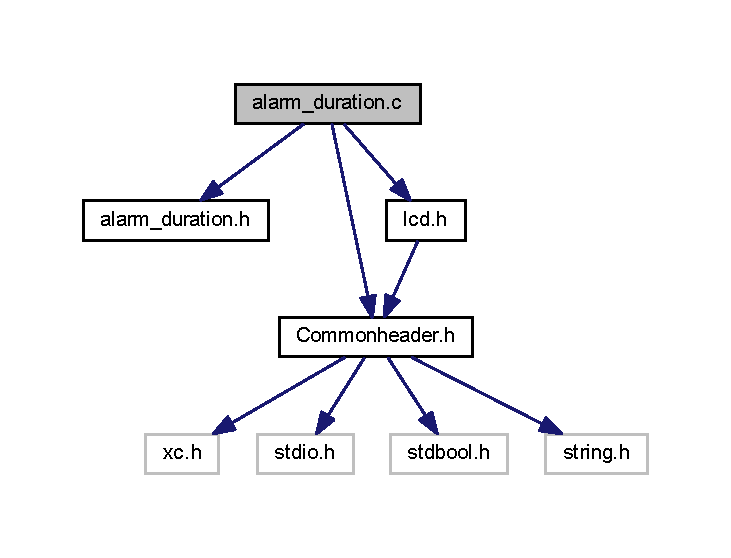
\includegraphics[width=350pt]{a00003}
\end{center}
\end{figure}
\subsubsection*{Macros}
\begin{DoxyCompactItemize}
\item 
\#define \textbf{ I\+N\+C\+R\+E\+M\+E\+N\+T\+\_\+\+M\+I\+N\+U\+T\+ES}~0x01
\item 
\#define \textbf{ D\+E\+C\+R\+E\+M\+E\+N\+T\+\_\+\+M\+I\+N\+U\+T\+ES}~0x02
\item 
\#define \textbf{ I\+N\+C\+R\+E\+M\+E\+N\+T\+\_\+\+S\+E\+C\+O\+N\+DS}~0x04
\item 
\#define \textbf{ D\+E\+C\+R\+E\+M\+E\+N\+T\+\_\+\+S\+E\+C\+O\+N\+DS}~0x08
\item 
\#define \textbf{ S\+A\+V\+E\+\_\+\+D\+U\+R\+A\+T\+I\+ON}~0x10
\end{DoxyCompactItemize}
\subsubsection*{Functions}
\begin{DoxyCompactItemize}
\item 
void \textbf{ alarm\+\_\+duration\+\_\+settings\+\_\+page} ()
\end{DoxyCompactItemize}
\subsubsection*{Variables}
\begin{DoxyCompactItemize}
\item 
bool \textbf{ quit}
\item 
\textbf{ Date\+Time} \textbf{ alarm\+Duration}
\end{DoxyCompactItemize}


\subsubsection{Macro Definition Documentation}
\mbox{\label{a00002_acc0fb1eee8deff23f5172ddd3b90b754}} 
\index{alarm\+\_\+duration.\+c@{alarm\+\_\+duration.\+c}!D\+E\+C\+R\+E\+M\+E\+N\+T\+\_\+\+M\+I\+N\+U\+T\+ES@{D\+E\+C\+R\+E\+M\+E\+N\+T\+\_\+\+M\+I\+N\+U\+T\+ES}}
\index{D\+E\+C\+R\+E\+M\+E\+N\+T\+\_\+\+M\+I\+N\+U\+T\+ES@{D\+E\+C\+R\+E\+M\+E\+N\+T\+\_\+\+M\+I\+N\+U\+T\+ES}!alarm\+\_\+duration.\+c@{alarm\+\_\+duration.\+c}}
\paragraph{D\+E\+C\+R\+E\+M\+E\+N\+T\+\_\+\+M\+I\+N\+U\+T\+ES}
{\footnotesize\ttfamily \#define D\+E\+C\+R\+E\+M\+E\+N\+T\+\_\+\+M\+I\+N\+U\+T\+ES~0x02}

\mbox{\label{a00002_a6c5f782df537f7854f6531797fa5c183}} 
\index{alarm\+\_\+duration.\+c@{alarm\+\_\+duration.\+c}!D\+E\+C\+R\+E\+M\+E\+N\+T\+\_\+\+S\+E\+C\+O\+N\+DS@{D\+E\+C\+R\+E\+M\+E\+N\+T\+\_\+\+S\+E\+C\+O\+N\+DS}}
\index{D\+E\+C\+R\+E\+M\+E\+N\+T\+\_\+\+S\+E\+C\+O\+N\+DS@{D\+E\+C\+R\+E\+M\+E\+N\+T\+\_\+\+S\+E\+C\+O\+N\+DS}!alarm\+\_\+duration.\+c@{alarm\+\_\+duration.\+c}}
\paragraph{D\+E\+C\+R\+E\+M\+E\+N\+T\+\_\+\+S\+E\+C\+O\+N\+DS}
{\footnotesize\ttfamily \#define D\+E\+C\+R\+E\+M\+E\+N\+T\+\_\+\+S\+E\+C\+O\+N\+DS~0x08}

\mbox{\label{a00002_a7766f73f1e8b4b229d8850a1957b182b}} 
\index{alarm\+\_\+duration.\+c@{alarm\+\_\+duration.\+c}!I\+N\+C\+R\+E\+M\+E\+N\+T\+\_\+\+M\+I\+N\+U\+T\+ES@{I\+N\+C\+R\+E\+M\+E\+N\+T\+\_\+\+M\+I\+N\+U\+T\+ES}}
\index{I\+N\+C\+R\+E\+M\+E\+N\+T\+\_\+\+M\+I\+N\+U\+T\+ES@{I\+N\+C\+R\+E\+M\+E\+N\+T\+\_\+\+M\+I\+N\+U\+T\+ES}!alarm\+\_\+duration.\+c@{alarm\+\_\+duration.\+c}}
\paragraph{I\+N\+C\+R\+E\+M\+E\+N\+T\+\_\+\+M\+I\+N\+U\+T\+ES}
{\footnotesize\ttfamily \#define I\+N\+C\+R\+E\+M\+E\+N\+T\+\_\+\+M\+I\+N\+U\+T\+ES~0x01}

\mbox{\label{a00002_a4ad0fc3b9c9f838ac4ed4612bc0e6956}} 
\index{alarm\+\_\+duration.\+c@{alarm\+\_\+duration.\+c}!I\+N\+C\+R\+E\+M\+E\+N\+T\+\_\+\+S\+E\+C\+O\+N\+DS@{I\+N\+C\+R\+E\+M\+E\+N\+T\+\_\+\+S\+E\+C\+O\+N\+DS}}
\index{I\+N\+C\+R\+E\+M\+E\+N\+T\+\_\+\+S\+E\+C\+O\+N\+DS@{I\+N\+C\+R\+E\+M\+E\+N\+T\+\_\+\+S\+E\+C\+O\+N\+DS}!alarm\+\_\+duration.\+c@{alarm\+\_\+duration.\+c}}
\paragraph{I\+N\+C\+R\+E\+M\+E\+N\+T\+\_\+\+S\+E\+C\+O\+N\+DS}
{\footnotesize\ttfamily \#define I\+N\+C\+R\+E\+M\+E\+N\+T\+\_\+\+S\+E\+C\+O\+N\+DS~0x04}

\mbox{\label{a00002_ad3e3bf2c56a15bd578c00f02f4803c4a}} 
\index{alarm\+\_\+duration.\+c@{alarm\+\_\+duration.\+c}!S\+A\+V\+E\+\_\+\+D\+U\+R\+A\+T\+I\+ON@{S\+A\+V\+E\+\_\+\+D\+U\+R\+A\+T\+I\+ON}}
\index{S\+A\+V\+E\+\_\+\+D\+U\+R\+A\+T\+I\+ON@{S\+A\+V\+E\+\_\+\+D\+U\+R\+A\+T\+I\+ON}!alarm\+\_\+duration.\+c@{alarm\+\_\+duration.\+c}}
\paragraph{S\+A\+V\+E\+\_\+\+D\+U\+R\+A\+T\+I\+ON}
{\footnotesize\ttfamily \#define S\+A\+V\+E\+\_\+\+D\+U\+R\+A\+T\+I\+ON~0x10}



\subsubsection{Function Documentation}
\mbox{\label{a00002_adc10f1c6bb2de8f4dd4d65901c941c0f}} 
\index{alarm\+\_\+duration.\+c@{alarm\+\_\+duration.\+c}!alarm\+\_\+duration\+\_\+settings\+\_\+page@{alarm\+\_\+duration\+\_\+settings\+\_\+page}}
\index{alarm\+\_\+duration\+\_\+settings\+\_\+page@{alarm\+\_\+duration\+\_\+settings\+\_\+page}!alarm\+\_\+duration.\+c@{alarm\+\_\+duration.\+c}}
\paragraph{alarm\+\_\+duration\+\_\+settings\+\_\+page()}
{\footnotesize\ttfamily void alarm\+\_\+duration\+\_\+settings\+\_\+page (\begin{DoxyParamCaption}{ }\end{DoxyParamCaption})}

Here is the call graph for this function\+:
\nopagebreak
\begin{figure}[H]
\begin{center}
\leavevmode
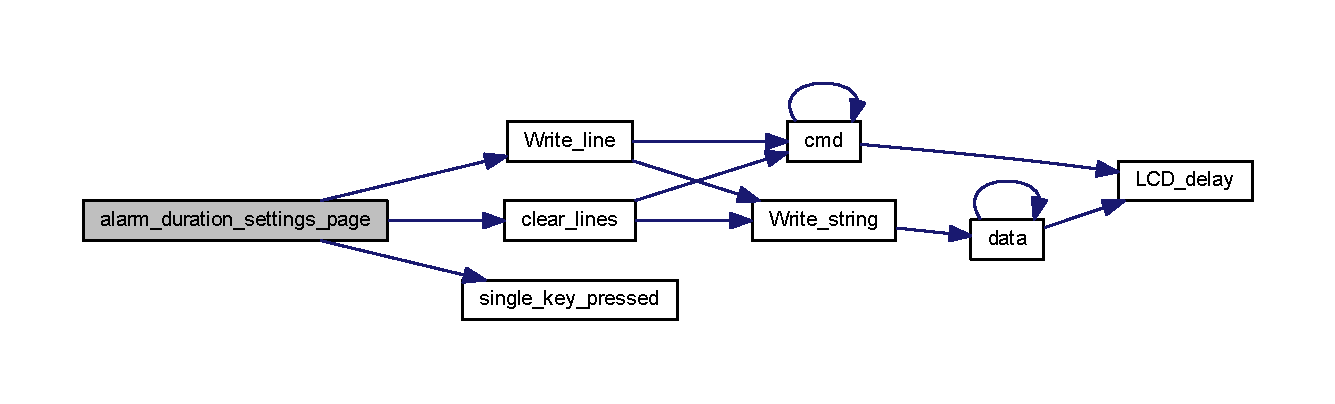
\includegraphics[width=350pt]{a00002_adc10f1c6bb2de8f4dd4d65901c941c0f_cgraph}
\end{center}
\end{figure}


\subsubsection{Variable Documentation}
\mbox{\label{a00002_a01c2a28170e998893c6428276cb87ae2}} 
\index{alarm\+\_\+duration.\+c@{alarm\+\_\+duration.\+c}!alarm\+Duration@{alarm\+Duration}}
\index{alarm\+Duration@{alarm\+Duration}!alarm\+\_\+duration.\+c@{alarm\+\_\+duration.\+c}}
\paragraph{alarm\+Duration}
{\footnotesize\ttfamily \textbf{ Date\+Time} alarm\+Duration}

\mbox{\label{a00002_ac746fa6ad48d19984a159f14bec028a3}} 
\index{alarm\+\_\+duration.\+c@{alarm\+\_\+duration.\+c}!quit@{quit}}
\index{quit@{quit}!alarm\+\_\+duration.\+c@{alarm\+\_\+duration.\+c}}
\paragraph{quit}
{\footnotesize\ttfamily bool quit}


\subsection{alarm\+\_\+duration.\+h File Reference}
\label{a00005}\index{alarm\+\_\+duration.\+h@{alarm\+\_\+duration.\+h}}
This graph shows which files directly or indirectly include this file\+:
\nopagebreak
\begin{figure}[H]
\begin{center}
\leavevmode
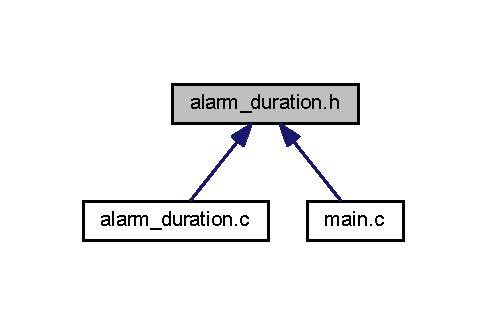
\includegraphics[width=234pt]{a00007}
\end{center}
\end{figure}
\subsubsection*{Functions}
\begin{DoxyCompactItemize}
\item 
void \textbf{ alarm\+\_\+duration\+\_\+settings\+\_\+page} ()
\end{DoxyCompactItemize}
\subsubsection*{Variables}
\begin{DoxyCompactItemize}
\item 
int \textbf{ current\+\_\+alarm\+\_\+duration}
\end{DoxyCompactItemize}


\subsubsection{Function Documentation}
\mbox{\label{a00005_adc10f1c6bb2de8f4dd4d65901c941c0f}} 
\index{alarm\+\_\+duration.\+h@{alarm\+\_\+duration.\+h}!alarm\+\_\+duration\+\_\+settings\+\_\+page@{alarm\+\_\+duration\+\_\+settings\+\_\+page}}
\index{alarm\+\_\+duration\+\_\+settings\+\_\+page@{alarm\+\_\+duration\+\_\+settings\+\_\+page}!alarm\+\_\+duration.\+h@{alarm\+\_\+duration.\+h}}
\paragraph{alarm\+\_\+duration\+\_\+settings\+\_\+page()}
{\footnotesize\ttfamily void alarm\+\_\+duration\+\_\+settings\+\_\+page (\begin{DoxyParamCaption}{ }\end{DoxyParamCaption})}

Here is the call graph for this function\+:
\nopagebreak
\begin{figure}[H]
\begin{center}
\leavevmode
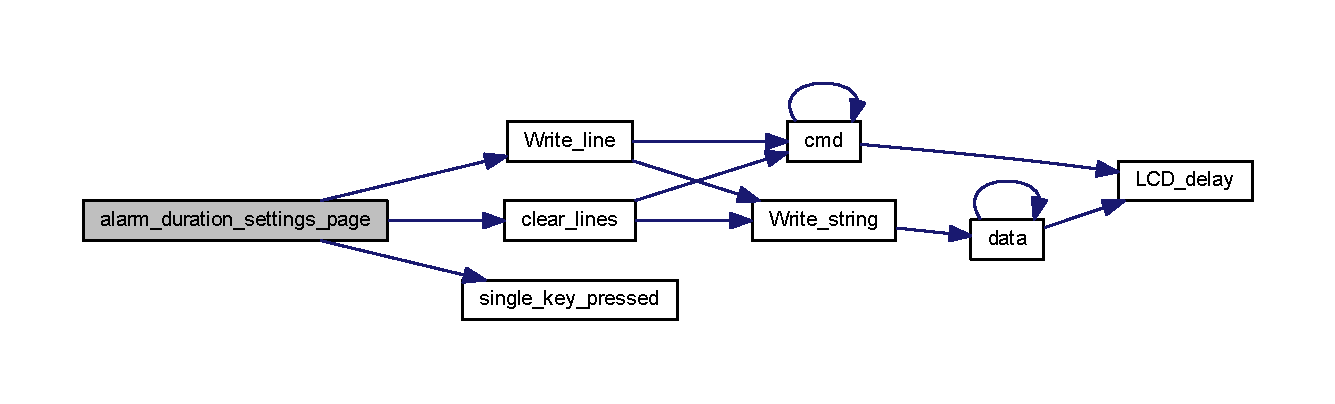
\includegraphics[width=350pt]{a00005_adc10f1c6bb2de8f4dd4d65901c941c0f_cgraph}
\end{center}
\end{figure}


\subsubsection{Variable Documentation}
\mbox{\label{a00005_ab073eeb8d5a2147ef91fab51d73ab4b2}} 
\index{alarm\+\_\+duration.\+h@{alarm\+\_\+duration.\+h}!current\+\_\+alarm\+\_\+duration@{current\+\_\+alarm\+\_\+duration}}
\index{current\+\_\+alarm\+\_\+duration@{current\+\_\+alarm\+\_\+duration}!alarm\+\_\+duration.\+h@{alarm\+\_\+duration.\+h}}
\paragraph{current\+\_\+alarm\+\_\+duration}
{\footnotesize\ttfamily int current\+\_\+alarm\+\_\+duration}


\subsection{buzzer.\+c File Reference}
\label{a00008}\index{buzzer.\+c@{buzzer.\+c}}
{\ttfamily \#include \char`\"{}buzzer.\+h\char`\"{}}\newline
{\ttfamily \#include \char`\"{}Commonheader.\+h\char`\"{}}\newline
{\ttfamily \#include \char`\"{}clock.\+h\char`\"{}}\newline
{\ttfamily \#include \char`\"{}lcd.\+h\char`\"{}}\newline
Include dependency graph for buzzer.\+c\+:
\nopagebreak
\begin{figure}[H]
\begin{center}
\leavevmode
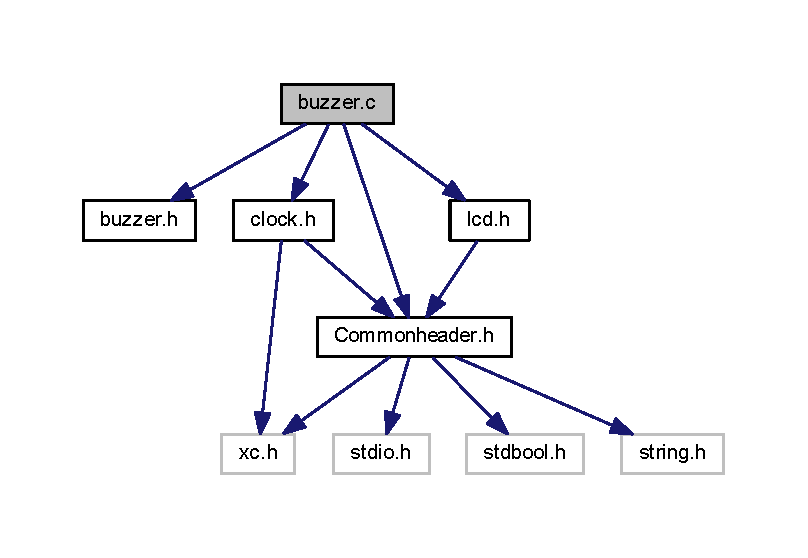
\includegraphics[width=350pt]{a00009}
\end{center}
\end{figure}
\subsubsection*{Functions}
\begin{DoxyCompactItemize}
\item 
void \textbf{ buzzer\+Init} ()
\item 
void \textbf{ sound\+Buzzer} (int duration, int zone)
\end{DoxyCompactItemize}
\subsubsection*{Variables}
\begin{DoxyCompactItemize}
\item 
int \textbf{ current\+\_\+alarm\+\_\+duration}
\item 
\textbf{ Date\+Time} \textbf{ alarm\+Duration}
\item 
bool \textbf{ quit}
\end{DoxyCompactItemize}


\subsubsection{Function Documentation}
\mbox{\label{a00008_ab39bc50f65525981c015786371a7892f}} 
\index{buzzer.\+c@{buzzer.\+c}!buzzer\+Init@{buzzer\+Init}}
\index{buzzer\+Init@{buzzer\+Init}!buzzer.\+c@{buzzer.\+c}}
\paragraph{buzzer\+Init()}
{\footnotesize\ttfamily void buzzer\+Init (\begin{DoxyParamCaption}{ }\end{DoxyParamCaption})}

Here is the caller graph for this function\+:
\nopagebreak
\begin{figure}[H]
\begin{center}
\leavevmode
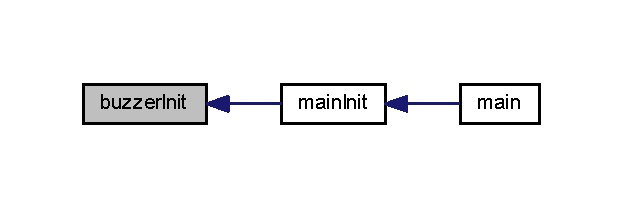
\includegraphics[width=299pt]{a00008_ab39bc50f65525981c015786371a7892f_icgraph}
\end{center}
\end{figure}
\mbox{\label{a00008_a31aed89a0638f80bd71a31c50f5cb3ff}} 
\index{buzzer.\+c@{buzzer.\+c}!sound\+Buzzer@{sound\+Buzzer}}
\index{sound\+Buzzer@{sound\+Buzzer}!buzzer.\+c@{buzzer.\+c}}
\paragraph{sound\+Buzzer()}
{\footnotesize\ttfamily void sound\+Buzzer (\begin{DoxyParamCaption}\item[{int}]{duration,  }\item[{int}]{zone }\end{DoxyParamCaption})}

Here is the call graph for this function\+:
\nopagebreak
\begin{figure}[H]
\begin{center}
\leavevmode
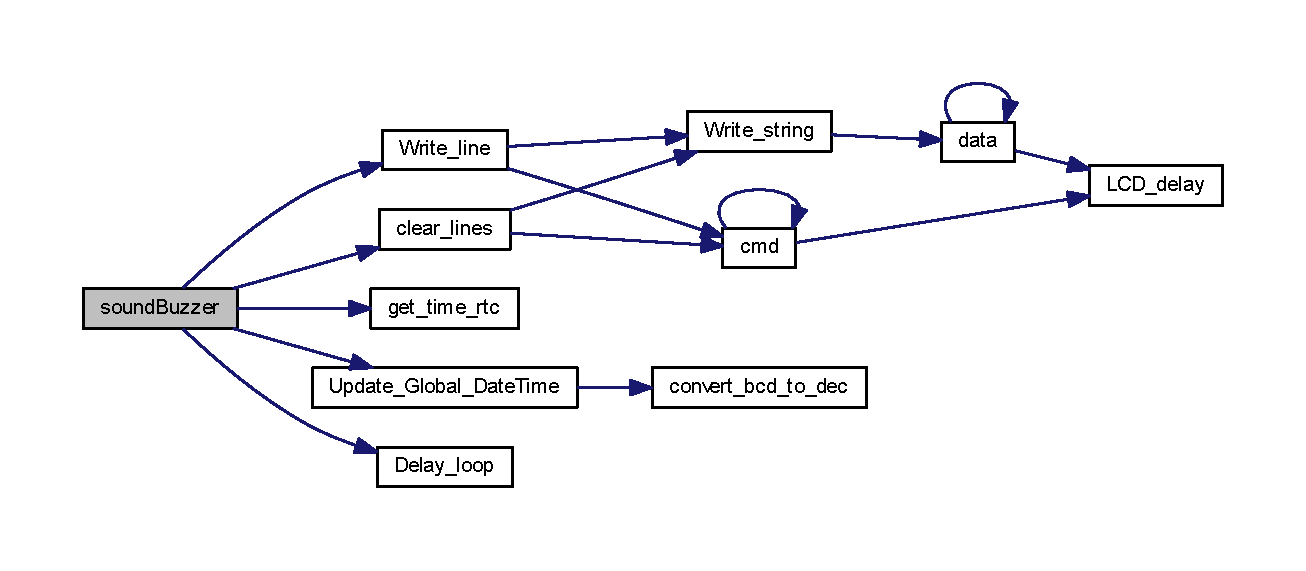
\includegraphics[width=350pt]{a00008_a31aed89a0638f80bd71a31c50f5cb3ff_cgraph}
\end{center}
\end{figure}
Here is the caller graph for this function\+:
\nopagebreak
\begin{figure}[H]
\begin{center}
\leavevmode
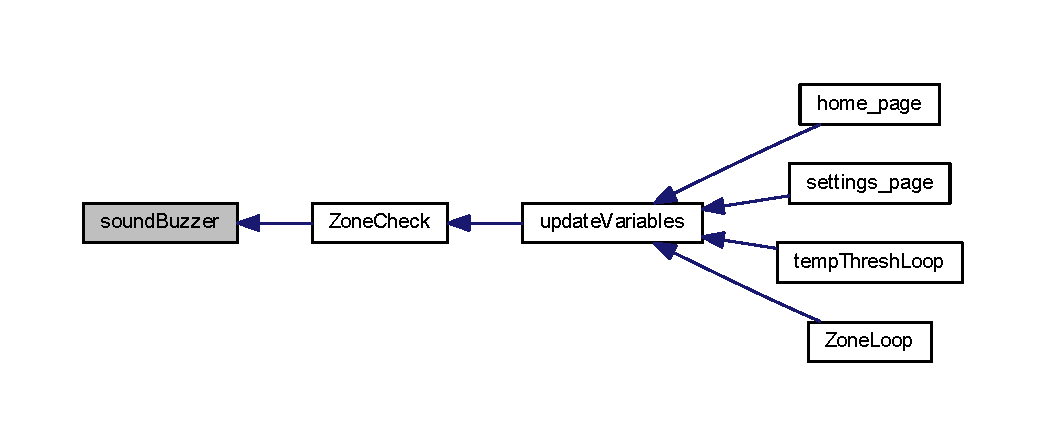
\includegraphics[width=350pt]{a00008_a31aed89a0638f80bd71a31c50f5cb3ff_icgraph}
\end{center}
\end{figure}


\subsubsection{Variable Documentation}
\mbox{\label{a00008_a01c2a28170e998893c6428276cb87ae2}} 
\index{buzzer.\+c@{buzzer.\+c}!alarm\+Duration@{alarm\+Duration}}
\index{alarm\+Duration@{alarm\+Duration}!buzzer.\+c@{buzzer.\+c}}
\paragraph{alarm\+Duration}
{\footnotesize\ttfamily \textbf{ Date\+Time} alarm\+Duration}

\mbox{\label{a00008_ab073eeb8d5a2147ef91fab51d73ab4b2}} 
\index{buzzer.\+c@{buzzer.\+c}!current\+\_\+alarm\+\_\+duration@{current\+\_\+alarm\+\_\+duration}}
\index{current\+\_\+alarm\+\_\+duration@{current\+\_\+alarm\+\_\+duration}!buzzer.\+c@{buzzer.\+c}}
\paragraph{current\+\_\+alarm\+\_\+duration}
{\footnotesize\ttfamily int current\+\_\+alarm\+\_\+duration}

\mbox{\label{a00008_ac746fa6ad48d19984a159f14bec028a3}} 
\index{buzzer.\+c@{buzzer.\+c}!quit@{quit}}
\index{quit@{quit}!buzzer.\+c@{buzzer.\+c}}
\paragraph{quit}
{\footnotesize\ttfamily bool quit}


\subsection{buzzer.\+h File Reference}
\label{a00011}\index{buzzer.\+h@{buzzer.\+h}}
This graph shows which files directly or indirectly include this file\+:
\nopagebreak
\begin{figure}[H]
\begin{center}
\leavevmode
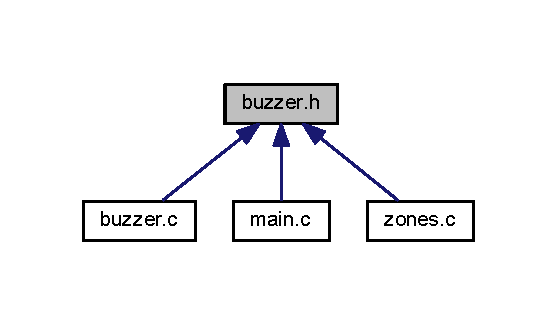
\includegraphics[width=268pt]{a00013}
\end{center}
\end{figure}
\subsubsection*{Macros}
\begin{DoxyCompactItemize}
\item 
\#define \textbf{ pin}~R\+C5
\end{DoxyCompactItemize}
\subsubsection*{Functions}
\begin{DoxyCompactItemize}
\item 
void \textbf{ sound\+Buzzer} (int duration, int zone)
\item 
void \textbf{ buzzer\+Init} ()
\end{DoxyCompactItemize}


\subsubsection{Macro Definition Documentation}
\mbox{\label{a00011_ab8451cb6d236c9f6399f800d36163767}} 
\index{buzzer.\+h@{buzzer.\+h}!pin@{pin}}
\index{pin@{pin}!buzzer.\+h@{buzzer.\+h}}
\paragraph{pin}
{\footnotesize\ttfamily \#define pin~R\+C5}



\subsubsection{Function Documentation}
\mbox{\label{a00011_ab39bc50f65525981c015786371a7892f}} 
\index{buzzer.\+h@{buzzer.\+h}!buzzer\+Init@{buzzer\+Init}}
\index{buzzer\+Init@{buzzer\+Init}!buzzer.\+h@{buzzer.\+h}}
\paragraph{buzzer\+Init()}
{\footnotesize\ttfamily void buzzer\+Init (\begin{DoxyParamCaption}{ }\end{DoxyParamCaption})}

Here is the caller graph for this function\+:
\nopagebreak
\begin{figure}[H]
\begin{center}
\leavevmode
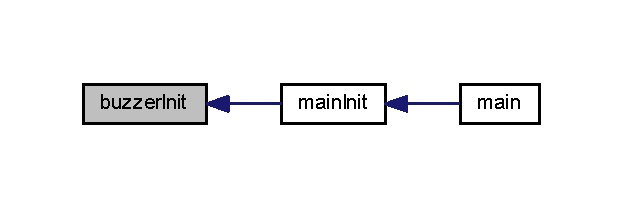
\includegraphics[width=299pt]{a00011_ab39bc50f65525981c015786371a7892f_icgraph}
\end{center}
\end{figure}
\mbox{\label{a00011_a31aed89a0638f80bd71a31c50f5cb3ff}} 
\index{buzzer.\+h@{buzzer.\+h}!sound\+Buzzer@{sound\+Buzzer}}
\index{sound\+Buzzer@{sound\+Buzzer}!buzzer.\+h@{buzzer.\+h}}
\paragraph{sound\+Buzzer()}
{\footnotesize\ttfamily void sound\+Buzzer (\begin{DoxyParamCaption}\item[{int}]{duration,  }\item[{int}]{zone }\end{DoxyParamCaption})}

Here is the call graph for this function\+:
\nopagebreak
\begin{figure}[H]
\begin{center}
\leavevmode
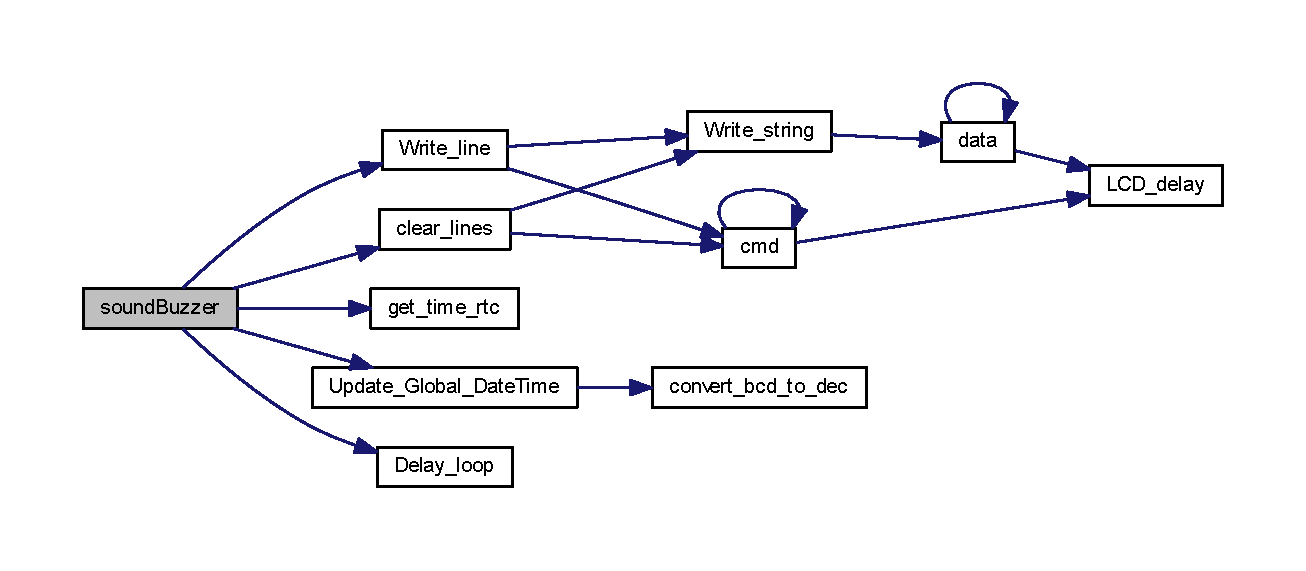
\includegraphics[width=350pt]{a00011_a31aed89a0638f80bd71a31c50f5cb3ff_cgraph}
\end{center}
\end{figure}
Here is the caller graph for this function\+:
\nopagebreak
\begin{figure}[H]
\begin{center}
\leavevmode
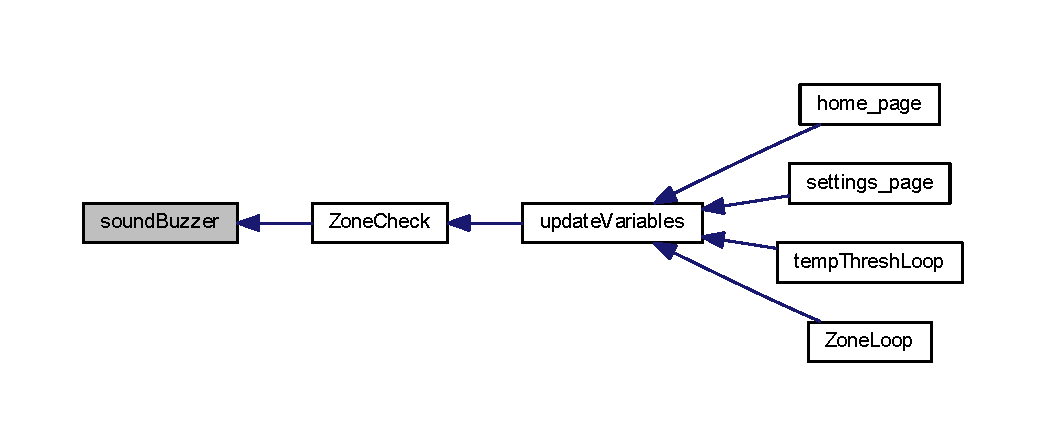
\includegraphics[width=350pt]{a00011_a31aed89a0638f80bd71a31c50f5cb3ff_icgraph}
\end{center}
\end{figure}

\subsection{clock.\+c File Reference}
\label{a00014}\index{clock.\+c@{clock.\+c}}
{\ttfamily \#include \char`\"{}Commonheader.\+h\char`\"{}}\newline
{\ttfamily \#include \char`\"{}clock.\+h\char`\"{}}\newline
{\ttfamily \#include $<$string.\+h$>$}\newline
{\ttfamily \#include $<$stdio.\+h$>$}\newline
Include dependency graph for clock.\+c\+:
\nopagebreak
\begin{figure}[H]
\begin{center}
\leavevmode
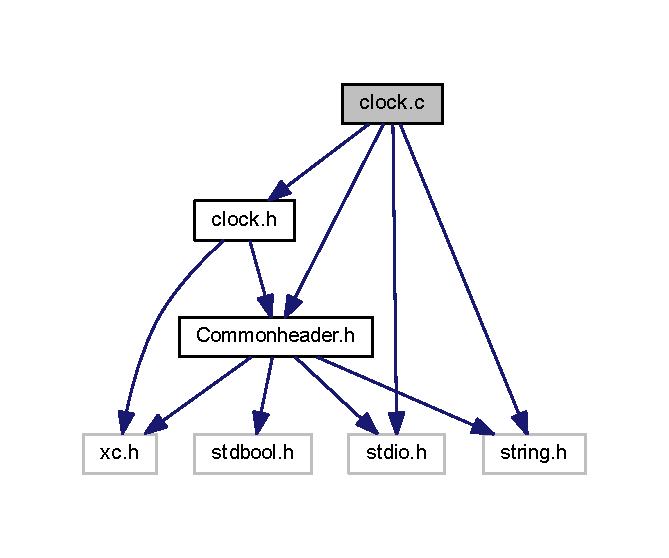
\includegraphics[width=321pt]{a00015}
\end{center}
\end{figure}
\subsubsection*{Functions}
\begin{DoxyCompactItemize}
\item 
void \textbf{ ds1302\+\_\+init} ()
\item 
void \textbf{ set\+\_\+time\+\_\+rtc} ()
\item 
void \textbf{ get\+\_\+time\+\_\+rtc} ()
\item 
void \textbf{ write\+\_\+time\+\_\+rtc} (unsigned char time\+\_\+tx)
\item 
unsigned char \textbf{ read\+\_\+time\+\_\+rtc} ()
\item 
void \textbf{ port\+\_\+init\+\_\+rtc} ()
\item 
void \textbf{ delay\+\_\+rtc} ()
\item 
void \textbf{ Write\+\_\+updated\+\_\+date\+\_\+time\+\_\+rtc} (\textbf{ Date\+Time} $\ast$\textbf{ date})
\item 
void \textbf{ Write\+\_\+updated\+\_\+date\+\_\+rtc} (\textbf{ Date\+Time} $\ast$\textbf{ date})
\item 
void \textbf{ Write\+\_\+updated\+\_\+time\+\_\+rtc} (\textbf{ Date\+Time} $\ast$\textbf{ date})
\item 
void \textbf{ Update\+\_\+\+Global\+\_\+\+Date\+Time} ()
\end{DoxyCompactItemize}


\subsubsection{Function Documentation}
\mbox{\label{a00014_a30a11d605a2fcfe8fc79c4f0a17a20cf}} 
\index{clock.\+c@{clock.\+c}!delay\+\_\+rtc@{delay\+\_\+rtc}}
\index{delay\+\_\+rtc@{delay\+\_\+rtc}!clock.\+c@{clock.\+c}}
\paragraph{delay\+\_\+rtc()}
{\footnotesize\ttfamily void delay\+\_\+rtc (\begin{DoxyParamCaption}{ }\end{DoxyParamCaption})}

\mbox{\label{a00014_a0665eb059e742e4bb5a419144336e147}} 
\index{clock.\+c@{clock.\+c}!ds1302\+\_\+init@{ds1302\+\_\+init}}
\index{ds1302\+\_\+init@{ds1302\+\_\+init}!clock.\+c@{clock.\+c}}
\paragraph{ds1302\+\_\+init()}
{\footnotesize\ttfamily void ds1302\+\_\+init (\begin{DoxyParamCaption}{ }\end{DoxyParamCaption})}

Here is the caller graph for this function\+:
\nopagebreak
\begin{figure}[H]
\begin{center}
\leavevmode
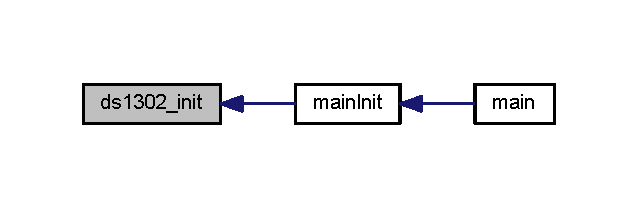
\includegraphics[width=306pt]{a00014_a0665eb059e742e4bb5a419144336e147_icgraph}
\end{center}
\end{figure}
\mbox{\label{a00014_a628868f4036626e8fa1b055bf56dc2f1}} 
\index{clock.\+c@{clock.\+c}!get\+\_\+time\+\_\+rtc@{get\+\_\+time\+\_\+rtc}}
\index{get\+\_\+time\+\_\+rtc@{get\+\_\+time\+\_\+rtc}!clock.\+c@{clock.\+c}}
\paragraph{get\+\_\+time\+\_\+rtc()}
{\footnotesize\ttfamily void get\+\_\+time\+\_\+rtc (\begin{DoxyParamCaption}{ }\end{DoxyParamCaption})}

Here is the caller graph for this function\+:
\nopagebreak
\begin{figure}[H]
\begin{center}
\leavevmode
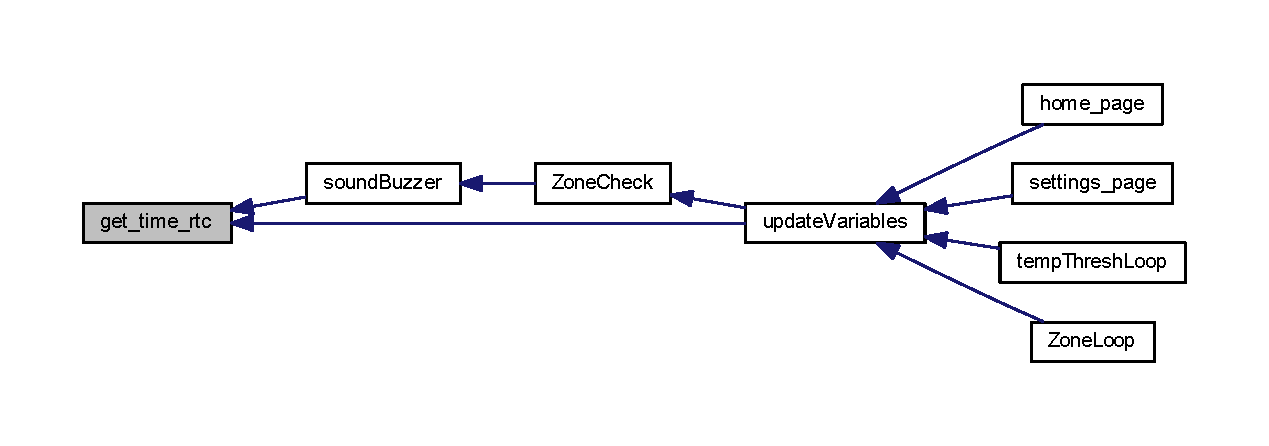
\includegraphics[width=350pt]{a00014_a628868f4036626e8fa1b055bf56dc2f1_icgraph}
\end{center}
\end{figure}
\mbox{\label{a00014_a4144a5333b1a934957b78e4b2d0f8695}} 
\index{clock.\+c@{clock.\+c}!port\+\_\+init\+\_\+rtc@{port\+\_\+init\+\_\+rtc}}
\index{port\+\_\+init\+\_\+rtc@{port\+\_\+init\+\_\+rtc}!clock.\+c@{clock.\+c}}
\paragraph{port\+\_\+init\+\_\+rtc()}
{\footnotesize\ttfamily void port\+\_\+init\+\_\+rtc (\begin{DoxyParamCaption}{ }\end{DoxyParamCaption})}

Here is the caller graph for this function\+:
\nopagebreak
\begin{figure}[H]
\begin{center}
\leavevmode
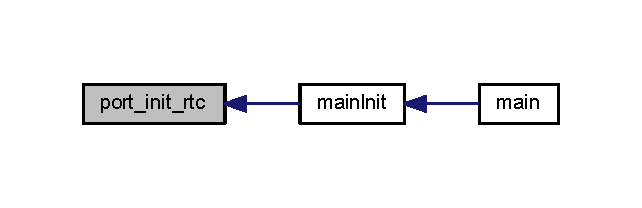
\includegraphics[width=308pt]{a00014_a4144a5333b1a934957b78e4b2d0f8695_icgraph}
\end{center}
\end{figure}
\mbox{\label{a00014_add06d1f93d90576fa369c2401c1d4aed}} 
\index{clock.\+c@{clock.\+c}!read\+\_\+time\+\_\+rtc@{read\+\_\+time\+\_\+rtc}}
\index{read\+\_\+time\+\_\+rtc@{read\+\_\+time\+\_\+rtc}!clock.\+c@{clock.\+c}}
\paragraph{read\+\_\+time\+\_\+rtc()}
{\footnotesize\ttfamily unsigned char read\+\_\+time\+\_\+rtc (\begin{DoxyParamCaption}{ }\end{DoxyParamCaption})}

Here is the call graph for this function\+:
\nopagebreak
\begin{figure}[H]
\begin{center}
\leavevmode
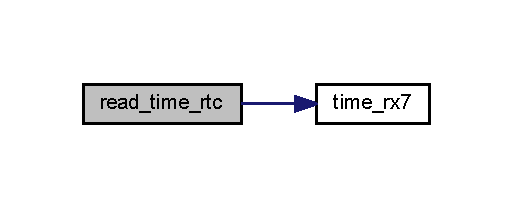
\includegraphics[width=246pt]{a00014_add06d1f93d90576fa369c2401c1d4aed_cgraph}
\end{center}
\end{figure}
Here is the caller graph for this function\+:
\nopagebreak
\begin{figure}[H]
\begin{center}
\leavevmode
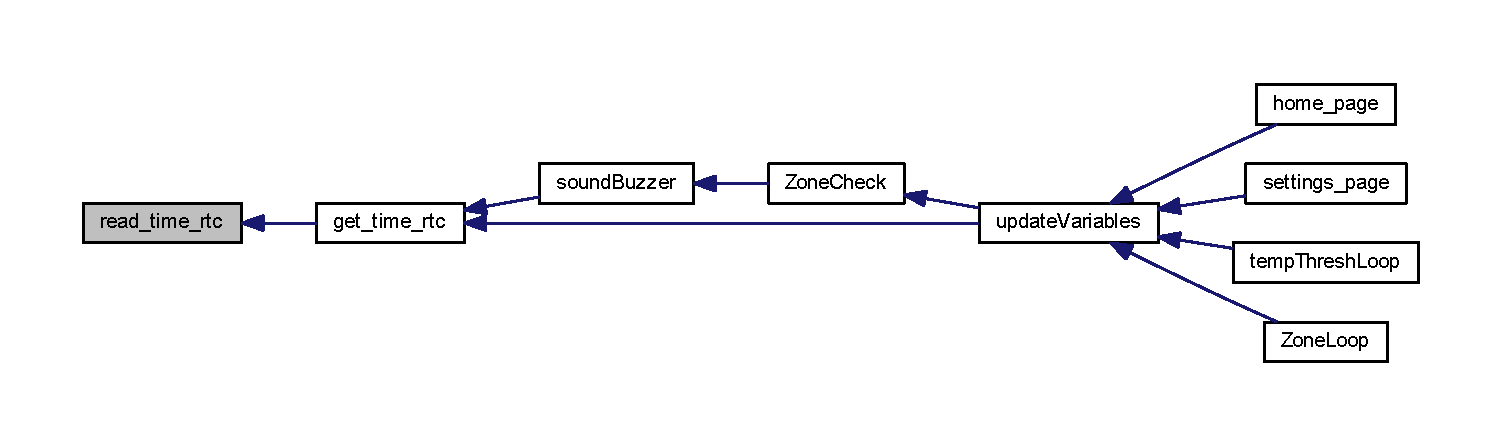
\includegraphics[width=350pt]{a00014_add06d1f93d90576fa369c2401c1d4aed_icgraph}
\end{center}
\end{figure}
\mbox{\label{a00014_af48611801cb8ae30f21f4263183355a4}} 
\index{clock.\+c@{clock.\+c}!set\+\_\+time\+\_\+rtc@{set\+\_\+time\+\_\+rtc}}
\index{set\+\_\+time\+\_\+rtc@{set\+\_\+time\+\_\+rtc}!clock.\+c@{clock.\+c}}
\paragraph{set\+\_\+time\+\_\+rtc()}
{\footnotesize\ttfamily void set\+\_\+time\+\_\+rtc (\begin{DoxyParamCaption}{ }\end{DoxyParamCaption})}

Here is the caller graph for this function\+:
\nopagebreak
\begin{figure}[H]
\begin{center}
\leavevmode
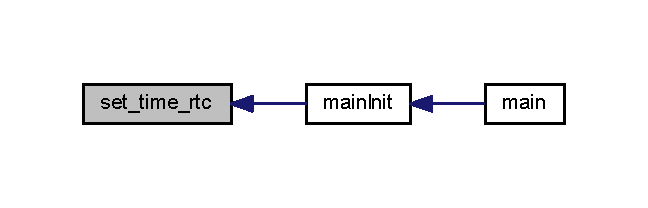
\includegraphics[width=311pt]{a00014_af48611801cb8ae30f21f4263183355a4_icgraph}
\end{center}
\end{figure}
\mbox{\label{a00014_a93b2ace39d0d582b18b136c908d8f092}} 
\index{clock.\+c@{clock.\+c}!Update\+\_\+\+Global\+\_\+\+Date\+Time@{Update\+\_\+\+Global\+\_\+\+Date\+Time}}
\index{Update\+\_\+\+Global\+\_\+\+Date\+Time@{Update\+\_\+\+Global\+\_\+\+Date\+Time}!clock.\+c@{clock.\+c}}
\paragraph{Update\+\_\+\+Global\+\_\+\+Date\+Time()}
{\footnotesize\ttfamily void Update\+\_\+\+Global\+\_\+\+Date\+Time (\begin{DoxyParamCaption}{ }\end{DoxyParamCaption})}

Here is the call graph for this function\+:
\nopagebreak
\begin{figure}[H]
\begin{center}
\leavevmode
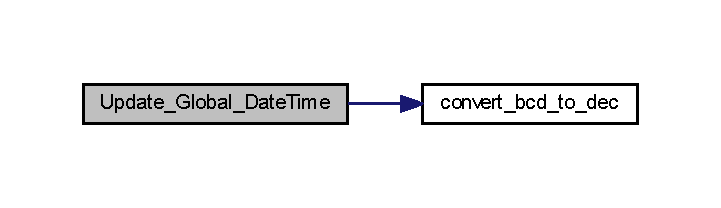
\includegraphics[width=346pt]{a00014_a93b2ace39d0d582b18b136c908d8f092_cgraph}
\end{center}
\end{figure}
Here is the caller graph for this function\+:
\nopagebreak
\begin{figure}[H]
\begin{center}
\leavevmode
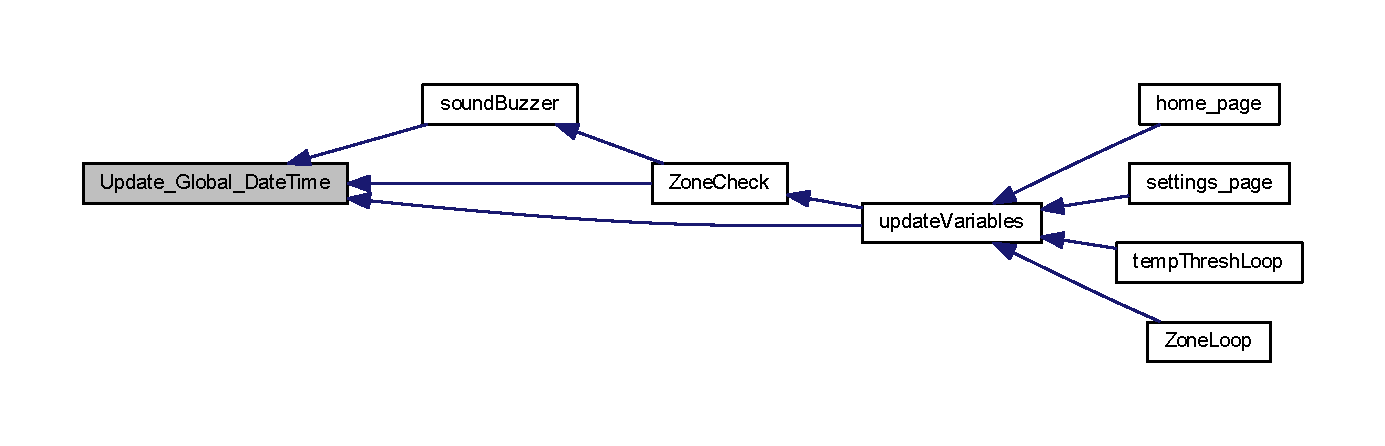
\includegraphics[width=350pt]{a00014_a93b2ace39d0d582b18b136c908d8f092_icgraph}
\end{center}
\end{figure}
\mbox{\label{a00014_aadecf4eb7d23c63d1216ced71440654e}} 
\index{clock.\+c@{clock.\+c}!write\+\_\+time\+\_\+rtc@{write\+\_\+time\+\_\+rtc}}
\index{write\+\_\+time\+\_\+rtc@{write\+\_\+time\+\_\+rtc}!clock.\+c@{clock.\+c}}
\paragraph{write\+\_\+time\+\_\+rtc()}
{\footnotesize\ttfamily void write\+\_\+time\+\_\+rtc (\begin{DoxyParamCaption}\item[{unsigned char}]{time\+\_\+tx }\end{DoxyParamCaption})}

Here is the caller graph for this function\+:
\nopagebreak
\begin{figure}[H]
\begin{center}
\leavevmode
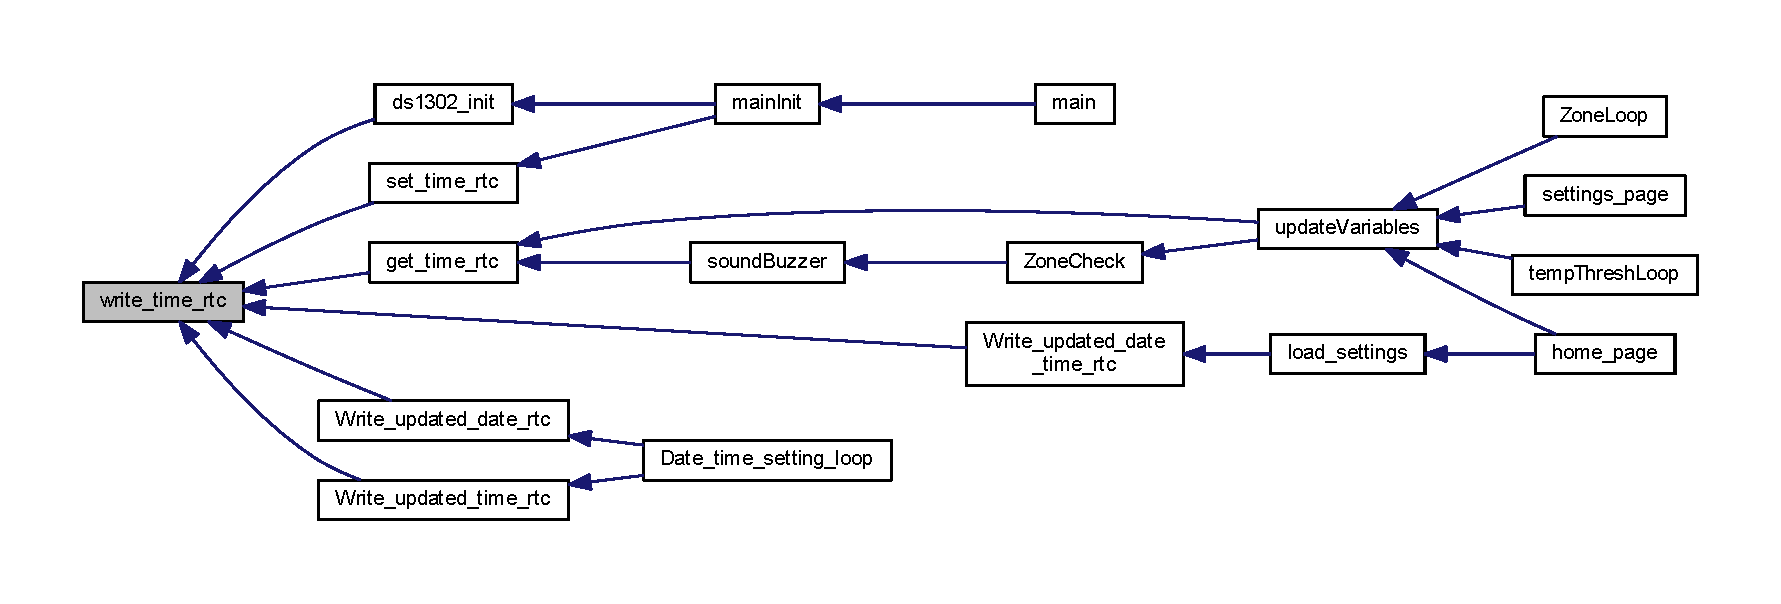
\includegraphics[width=350pt]{a00014_aadecf4eb7d23c63d1216ced71440654e_icgraph}
\end{center}
\end{figure}
\mbox{\label{a00014_a7ae143903216d08d3f0c07b95e21c21b}} 
\index{clock.\+c@{clock.\+c}!Write\+\_\+updated\+\_\+date\+\_\+rtc@{Write\+\_\+updated\+\_\+date\+\_\+rtc}}
\index{Write\+\_\+updated\+\_\+date\+\_\+rtc@{Write\+\_\+updated\+\_\+date\+\_\+rtc}!clock.\+c@{clock.\+c}}
\paragraph{Write\+\_\+updated\+\_\+date\+\_\+rtc()}
{\footnotesize\ttfamily void Write\+\_\+updated\+\_\+date\+\_\+rtc (\begin{DoxyParamCaption}\item[{\textbf{ Date\+Time} $\ast$}]{date }\end{DoxyParamCaption})}

Here is the call graph for this function\+:
\nopagebreak
\begin{figure}[H]
\begin{center}
\leavevmode
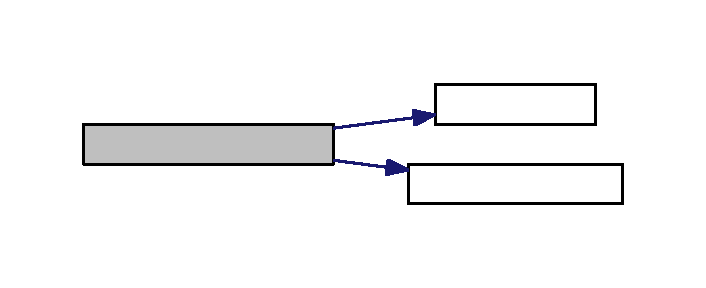
\includegraphics[width=339pt]{a00014_a7ae143903216d08d3f0c07b95e21c21b_cgraph}
\end{center}
\end{figure}
Here is the caller graph for this function\+:
\nopagebreak
\begin{figure}[H]
\begin{center}
\leavevmode
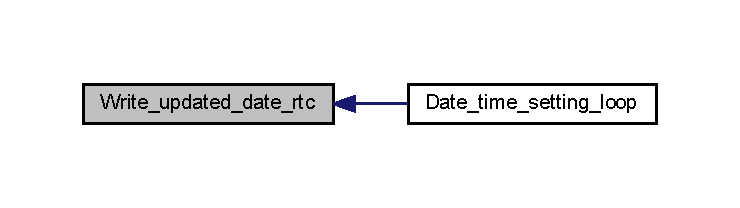
\includegraphics[width=350pt]{a00014_a7ae143903216d08d3f0c07b95e21c21b_icgraph}
\end{center}
\end{figure}
\mbox{\label{a00014_ad20fe32d70b509ba8f7f24a572e34f3f}} 
\index{clock.\+c@{clock.\+c}!Write\+\_\+updated\+\_\+date\+\_\+time\+\_\+rtc@{Write\+\_\+updated\+\_\+date\+\_\+time\+\_\+rtc}}
\index{Write\+\_\+updated\+\_\+date\+\_\+time\+\_\+rtc@{Write\+\_\+updated\+\_\+date\+\_\+time\+\_\+rtc}!clock.\+c@{clock.\+c}}
\paragraph{Write\+\_\+updated\+\_\+date\+\_\+time\+\_\+rtc()}
{\footnotesize\ttfamily void Write\+\_\+updated\+\_\+date\+\_\+time\+\_\+rtc (\begin{DoxyParamCaption}\item[{\textbf{ Date\+Time} $\ast$}]{date }\end{DoxyParamCaption})}

Here is the call graph for this function\+:
\nopagebreak
\begin{figure}[H]
\begin{center}
\leavevmode
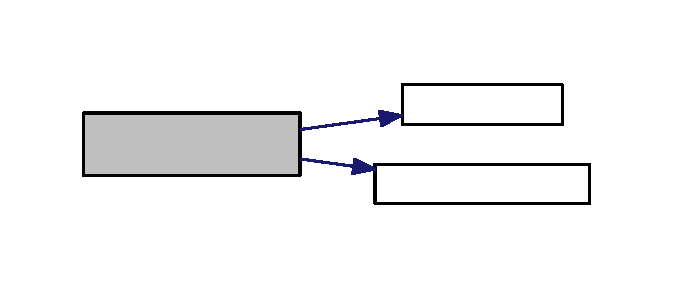
\includegraphics[width=323pt]{a00014_ad20fe32d70b509ba8f7f24a572e34f3f_cgraph}
\end{center}
\end{figure}
Here is the caller graph for this function\+:
\nopagebreak
\begin{figure}[H]
\begin{center}
\leavevmode
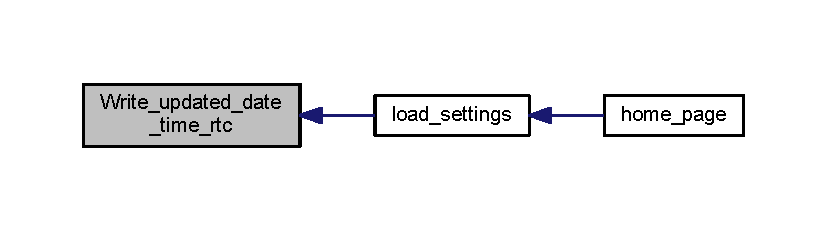
\includegraphics[width=350pt]{a00014_ad20fe32d70b509ba8f7f24a572e34f3f_icgraph}
\end{center}
\end{figure}
\mbox{\label{a00014_a2f6bf3793293cc3f2c09a91c3725a8af}} 
\index{clock.\+c@{clock.\+c}!Write\+\_\+updated\+\_\+time\+\_\+rtc@{Write\+\_\+updated\+\_\+time\+\_\+rtc}}
\index{Write\+\_\+updated\+\_\+time\+\_\+rtc@{Write\+\_\+updated\+\_\+time\+\_\+rtc}!clock.\+c@{clock.\+c}}
\paragraph{Write\+\_\+updated\+\_\+time\+\_\+rtc()}
{\footnotesize\ttfamily void Write\+\_\+updated\+\_\+time\+\_\+rtc (\begin{DoxyParamCaption}\item[{\textbf{ Date\+Time} $\ast$}]{date }\end{DoxyParamCaption})}

Here is the call graph for this function\+:
\nopagebreak
\begin{figure}[H]
\begin{center}
\leavevmode
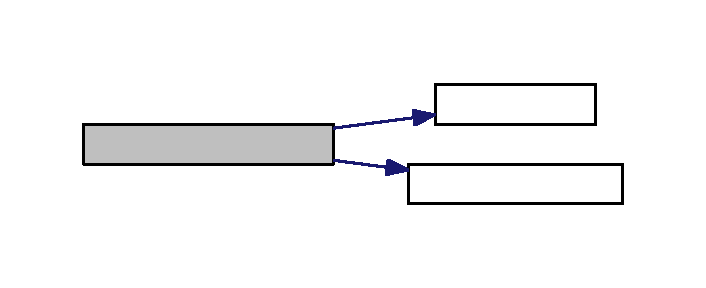
\includegraphics[width=339pt]{a00014_a2f6bf3793293cc3f2c09a91c3725a8af_cgraph}
\end{center}
\end{figure}
Here is the caller graph for this function\+:
\nopagebreak
\begin{figure}[H]
\begin{center}
\leavevmode
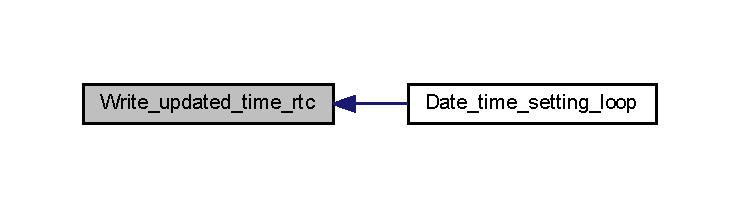
\includegraphics[width=350pt]{a00014_a2f6bf3793293cc3f2c09a91c3725a8af_icgraph}
\end{center}
\end{figure}

\subsection{clock.\+h File Reference}
\label{a00017}\index{clock.\+h@{clock.\+h}}
{\ttfamily \#include $<$xc.\+h$>$}\newline
{\ttfamily \#include \char`\"{}Commonheader.\+h\char`\"{}}\newline
Include dependency graph for clock.\+h\+:
\nopagebreak
\begin{figure}[H]
\begin{center}
\leavevmode
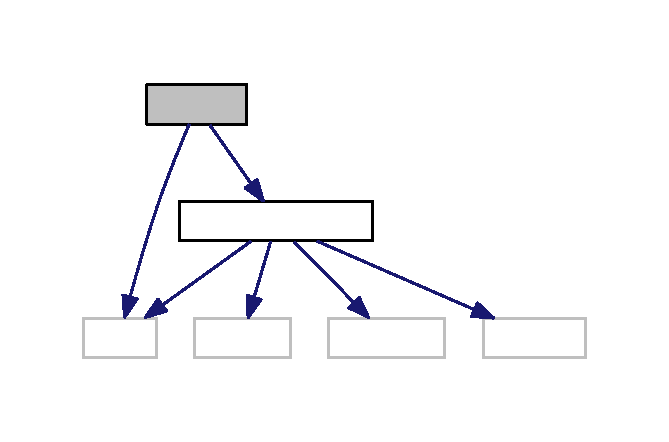
\includegraphics[width=321pt]{a00018}
\end{center}
\end{figure}
This graph shows which files directly or indirectly include this file\+:
\nopagebreak
\begin{figure}[H]
\begin{center}
\leavevmode
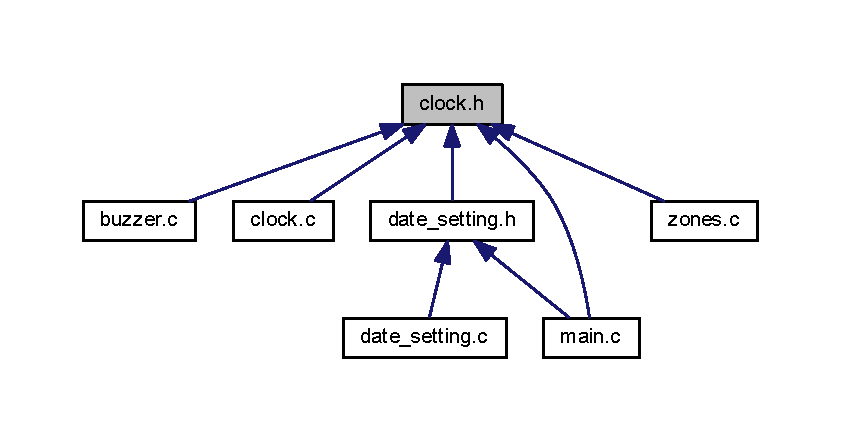
\includegraphics[width=350pt]{a00019}
\end{center}
\end{figure}
\subsubsection*{Macros}
\begin{DoxyCompactItemize}
\item 
\#define \textbf{ R\+T\+C\+\_\+\+IO}~R\+B4
\item 
\#define \textbf{ R\+T\+C\+\_\+\+C\+LK}~R\+C4
\item 
\#define \textbf{ R\+T\+C\+\_\+\+R\+ST}~R\+B5
\item 
\#define \textbf{ R\+T\+C\+\_\+\+C\+O\+N\+T\+R\+O\+L\+\_\+\+W\+R\+I\+TE}~0x8E
\item 
\#define \textbf{ R\+T\+C\+\_\+\+L\+O\+W\+\_\+\+M\+A\+SK}~0x0F
\item 
\#define \textbf{ R\+T\+C\+\_\+\+H\+I\+G\+H\+\_\+\+M\+A\+SK}~0x\+F0
\end{DoxyCompactItemize}
\subsubsection*{Functions}
\begin{DoxyCompactItemize}
\item 
bit \textbf{ time\+\_\+rx7} (unsigned) \&\textbf{ time\+\_\+rx} $\ast$8+7
\item 
void \textbf{ port\+\_\+init\+\_\+rtc} ()
\item 
void \textbf{ ds1302\+\_\+init} ()
\item 
void \textbf{ set\+\_\+time\+\_\+rtc} ()
\item 
void \textbf{ get\+\_\+time\+\_\+rtc} ()
\item 
void \textbf{ Update\+\_\+\+Global\+\_\+\+Date\+Time} ()
\item 
void \textbf{ Write\+\_\+updated\+\_\+date\+\_\+time\+\_\+rtc} (\textbf{ Date\+Time} $\ast$\textbf{ date})
\item 
void \textbf{ Write\+\_\+updated\+\_\+date\+\_\+rtc} (\textbf{ Date\+Time} $\ast$\textbf{ date})
\item 
void \textbf{ Write\+\_\+updated\+\_\+time\+\_\+rtc} (\textbf{ Date\+Time} $\ast$\textbf{ date})
\item 
void \textbf{ Write\+\_\+date\+Time\+\_\+rtc} (\textbf{ Date\+Time} $\ast$\textbf{ date})
\item 
void \textbf{ write\+\_\+time\+\_\+rtc} (unsigned char time\+\_\+tx)
\item 
unsigned char \textbf{ read\+\_\+time\+\_\+rtc} ()
\item 
void \textbf{ delay\+\_\+rtc} ()
\end{DoxyCompactItemize}
\subsubsection*{Variables}
\begin{DoxyCompactItemize}
\item 
unsigned char \textbf{ time\+\_\+rx}
\item 
const char \textbf{ rtc\+\_\+table} [$\,$] =\{0x00, 0x58, 0x12, 0x12, 0x12, 0x06, 0x17, 0x00\}
\item 
char \textbf{ rtc\+\_\+table1} [7]
\item 
char \textbf{ rtc\+\_\+lcd\+\_\+display\+\_\+date\+\_\+table} [9]
\item 
char \textbf{ rtc\+\_\+lcd\+\_\+display\+\_\+time\+\_\+table} [9]
\item 
const char \textbf{ rtc\+\_\+7\+\_\+seg\+\_\+display\+\_\+table} [$\,$] =\{0xc0,0xf9,0xa4,0xb0,0x99,0x92,0x82,0xf8,0x80,0x90\}
\item 
\textbf{ Date\+Time} \textbf{ date\+Time}
\item 
bool \textbf{ Date\+Changed}
\end{DoxyCompactItemize}


\subsubsection{Macro Definition Documentation}
\mbox{\label{a00017_a80e62c38e7452c92057864f26034ee82}} 
\index{clock.\+h@{clock.\+h}!R\+T\+C\+\_\+\+C\+LK@{R\+T\+C\+\_\+\+C\+LK}}
\index{R\+T\+C\+\_\+\+C\+LK@{R\+T\+C\+\_\+\+C\+LK}!clock.\+h@{clock.\+h}}
\paragraph{R\+T\+C\+\_\+\+C\+LK}
{\footnotesize\ttfamily \#define R\+T\+C\+\_\+\+C\+LK~R\+C4}

\mbox{\label{a00017_a089dd813e4790e77ef2b640e865cd390}} 
\index{clock.\+h@{clock.\+h}!R\+T\+C\+\_\+\+C\+O\+N\+T\+R\+O\+L\+\_\+\+W\+R\+I\+TE@{R\+T\+C\+\_\+\+C\+O\+N\+T\+R\+O\+L\+\_\+\+W\+R\+I\+TE}}
\index{R\+T\+C\+\_\+\+C\+O\+N\+T\+R\+O\+L\+\_\+\+W\+R\+I\+TE@{R\+T\+C\+\_\+\+C\+O\+N\+T\+R\+O\+L\+\_\+\+W\+R\+I\+TE}!clock.\+h@{clock.\+h}}
\paragraph{R\+T\+C\+\_\+\+C\+O\+N\+T\+R\+O\+L\+\_\+\+W\+R\+I\+TE}
{\footnotesize\ttfamily \#define R\+T\+C\+\_\+\+C\+O\+N\+T\+R\+O\+L\+\_\+\+W\+R\+I\+TE~0x8E}

\mbox{\label{a00017_af7f4ebf8c48ec52f601d7f0ab359887e}} 
\index{clock.\+h@{clock.\+h}!R\+T\+C\+\_\+\+H\+I\+G\+H\+\_\+\+M\+A\+SK@{R\+T\+C\+\_\+\+H\+I\+G\+H\+\_\+\+M\+A\+SK}}
\index{R\+T\+C\+\_\+\+H\+I\+G\+H\+\_\+\+M\+A\+SK@{R\+T\+C\+\_\+\+H\+I\+G\+H\+\_\+\+M\+A\+SK}!clock.\+h@{clock.\+h}}
\paragraph{R\+T\+C\+\_\+\+H\+I\+G\+H\+\_\+\+M\+A\+SK}
{\footnotesize\ttfamily \#define R\+T\+C\+\_\+\+H\+I\+G\+H\+\_\+\+M\+A\+SK~0x\+F0}

\mbox{\label{a00017_a4e7388c98e6856978dbc5b2e5cb5bed4}} 
\index{clock.\+h@{clock.\+h}!R\+T\+C\+\_\+\+IO@{R\+T\+C\+\_\+\+IO}}
\index{R\+T\+C\+\_\+\+IO@{R\+T\+C\+\_\+\+IO}!clock.\+h@{clock.\+h}}
\paragraph{R\+T\+C\+\_\+\+IO}
{\footnotesize\ttfamily \#define R\+T\+C\+\_\+\+IO~R\+B4}

\mbox{\label{a00017_a779d126cf8a210658268556194e708b3}} 
\index{clock.\+h@{clock.\+h}!R\+T\+C\+\_\+\+L\+O\+W\+\_\+\+M\+A\+SK@{R\+T\+C\+\_\+\+L\+O\+W\+\_\+\+M\+A\+SK}}
\index{R\+T\+C\+\_\+\+L\+O\+W\+\_\+\+M\+A\+SK@{R\+T\+C\+\_\+\+L\+O\+W\+\_\+\+M\+A\+SK}!clock.\+h@{clock.\+h}}
\paragraph{R\+T\+C\+\_\+\+L\+O\+W\+\_\+\+M\+A\+SK}
{\footnotesize\ttfamily \#define R\+T\+C\+\_\+\+L\+O\+W\+\_\+\+M\+A\+SK~0x0F}

\mbox{\label{a00017_a1615ada9d76f57d41ce419e9e1e25c8b}} 
\index{clock.\+h@{clock.\+h}!R\+T\+C\+\_\+\+R\+ST@{R\+T\+C\+\_\+\+R\+ST}}
\index{R\+T\+C\+\_\+\+R\+ST@{R\+T\+C\+\_\+\+R\+ST}!clock.\+h@{clock.\+h}}
\paragraph{R\+T\+C\+\_\+\+R\+ST}
{\footnotesize\ttfamily \#define R\+T\+C\+\_\+\+R\+ST~R\+B5}



\subsubsection{Function Documentation}
\mbox{\label{a00017_a30a11d605a2fcfe8fc79c4f0a17a20cf}} 
\index{clock.\+h@{clock.\+h}!delay\+\_\+rtc@{delay\+\_\+rtc}}
\index{delay\+\_\+rtc@{delay\+\_\+rtc}!clock.\+h@{clock.\+h}}
\paragraph{delay\+\_\+rtc()}
{\footnotesize\ttfamily void delay\+\_\+rtc (\begin{DoxyParamCaption}{ }\end{DoxyParamCaption})}

\mbox{\label{a00017_a0665eb059e742e4bb5a419144336e147}} 
\index{clock.\+h@{clock.\+h}!ds1302\+\_\+init@{ds1302\+\_\+init}}
\index{ds1302\+\_\+init@{ds1302\+\_\+init}!clock.\+h@{clock.\+h}}
\paragraph{ds1302\+\_\+init()}
{\footnotesize\ttfamily void ds1302\+\_\+init (\begin{DoxyParamCaption}{ }\end{DoxyParamCaption})}

\mbox{\label{a00017_a628868f4036626e8fa1b055bf56dc2f1}} 
\index{clock.\+h@{clock.\+h}!get\+\_\+time\+\_\+rtc@{get\+\_\+time\+\_\+rtc}}
\index{get\+\_\+time\+\_\+rtc@{get\+\_\+time\+\_\+rtc}!clock.\+h@{clock.\+h}}
\paragraph{get\+\_\+time\+\_\+rtc()}
{\footnotesize\ttfamily void get\+\_\+time\+\_\+rtc (\begin{DoxyParamCaption}{ }\end{DoxyParamCaption})}

\mbox{\label{a00017_a4144a5333b1a934957b78e4b2d0f8695}} 
\index{clock.\+h@{clock.\+h}!port\+\_\+init\+\_\+rtc@{port\+\_\+init\+\_\+rtc}}
\index{port\+\_\+init\+\_\+rtc@{port\+\_\+init\+\_\+rtc}!clock.\+h@{clock.\+h}}
\paragraph{port\+\_\+init\+\_\+rtc()}
{\footnotesize\ttfamily void port\+\_\+init\+\_\+rtc (\begin{DoxyParamCaption}{ }\end{DoxyParamCaption})}

\mbox{\label{a00017_add06d1f93d90576fa369c2401c1d4aed}} 
\index{clock.\+h@{clock.\+h}!read\+\_\+time\+\_\+rtc@{read\+\_\+time\+\_\+rtc}}
\index{read\+\_\+time\+\_\+rtc@{read\+\_\+time\+\_\+rtc}!clock.\+h@{clock.\+h}}
\paragraph{read\+\_\+time\+\_\+rtc()}
{\footnotesize\ttfamily unsigned char read\+\_\+time\+\_\+rtc (\begin{DoxyParamCaption}{ }\end{DoxyParamCaption})}

Here is the call graph for this function\+:
\nopagebreak
\begin{figure}[H]
\begin{center}
\leavevmode
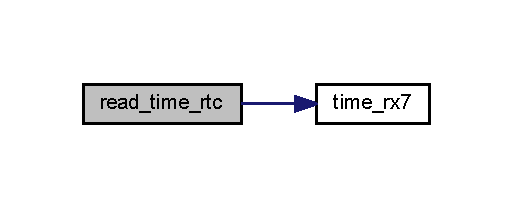
\includegraphics[width=246pt]{a00017_add06d1f93d90576fa369c2401c1d4aed_cgraph}
\end{center}
\end{figure}
Here is the caller graph for this function\+:
\nopagebreak
\begin{figure}[H]
\begin{center}
\leavevmode
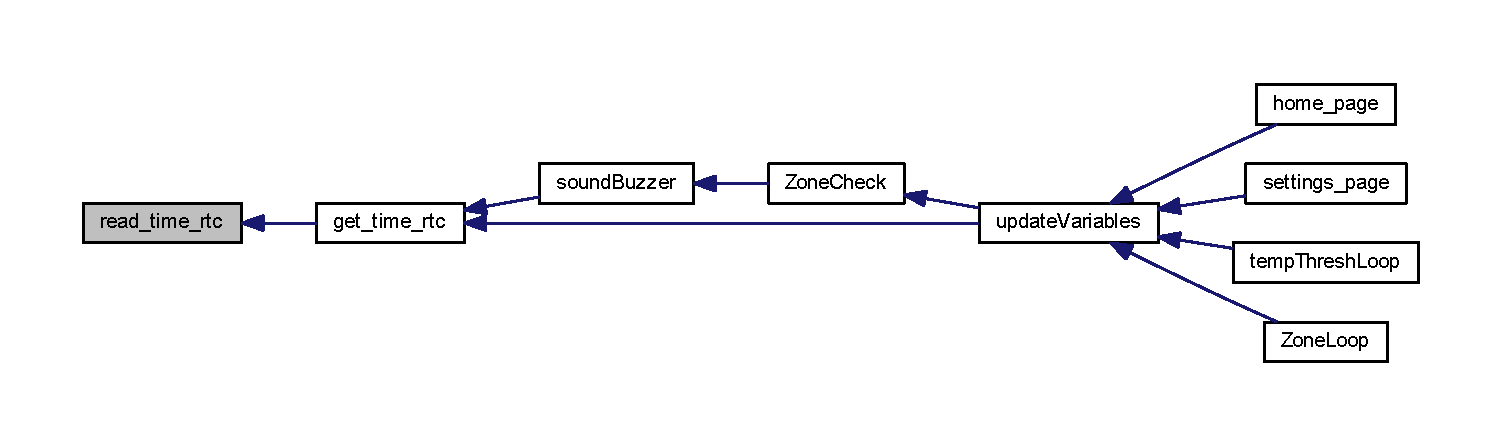
\includegraphics[width=350pt]{a00017_add06d1f93d90576fa369c2401c1d4aed_icgraph}
\end{center}
\end{figure}
\mbox{\label{a00017_af48611801cb8ae30f21f4263183355a4}} 
\index{clock.\+h@{clock.\+h}!set\+\_\+time\+\_\+rtc@{set\+\_\+time\+\_\+rtc}}
\index{set\+\_\+time\+\_\+rtc@{set\+\_\+time\+\_\+rtc}!clock.\+h@{clock.\+h}}
\paragraph{set\+\_\+time\+\_\+rtc()}
{\footnotesize\ttfamily void set\+\_\+time\+\_\+rtc (\begin{DoxyParamCaption}{ }\end{DoxyParamCaption})}

\mbox{\label{a00017_a64b918d8106cc55aaced41002a03eeec}} 
\index{clock.\+h@{clock.\+h}!time\+\_\+rx7@{time\+\_\+rx7}}
\index{time\+\_\+rx7@{time\+\_\+rx7}!clock.\+h@{clock.\+h}}
\paragraph{time\+\_\+rx7()}
{\footnotesize\ttfamily bit time\+\_\+rx7 (\begin{DoxyParamCaption}\item[{unsigned}]{ }\end{DoxyParamCaption}) \&}

Here is the caller graph for this function\+:
\nopagebreak
\begin{figure}[H]
\begin{center}
\leavevmode
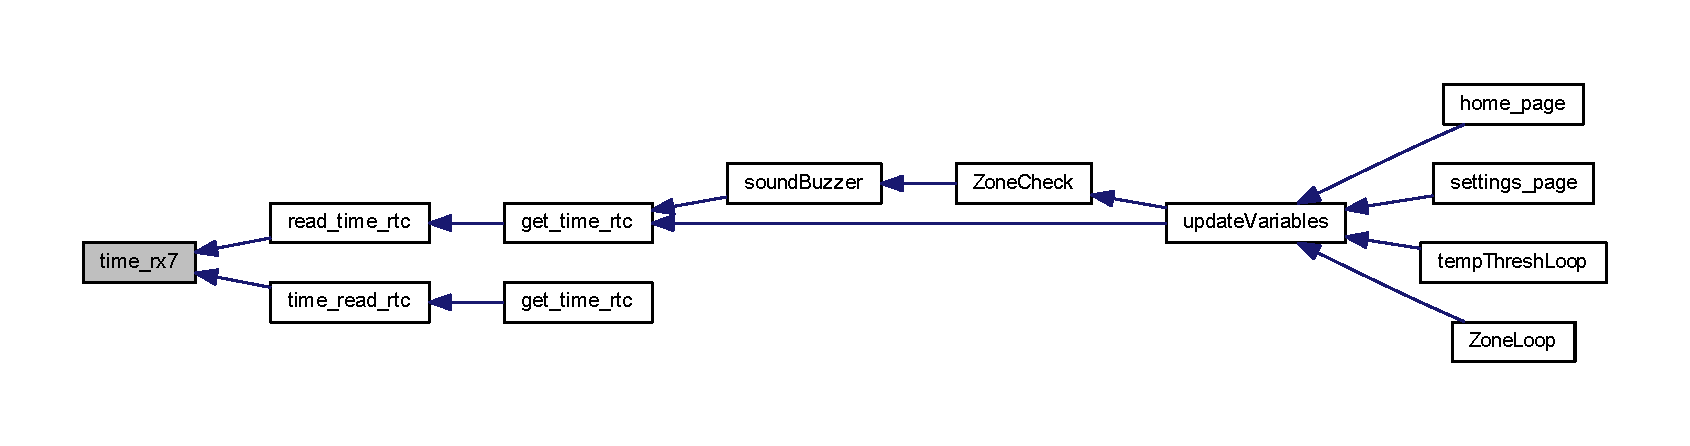
\includegraphics[width=350pt]{a00017_a64b918d8106cc55aaced41002a03eeec_icgraph}
\end{center}
\end{figure}
\mbox{\label{a00017_a93b2ace39d0d582b18b136c908d8f092}} 
\index{clock.\+h@{clock.\+h}!Update\+\_\+\+Global\+\_\+\+Date\+Time@{Update\+\_\+\+Global\+\_\+\+Date\+Time}}
\index{Update\+\_\+\+Global\+\_\+\+Date\+Time@{Update\+\_\+\+Global\+\_\+\+Date\+Time}!clock.\+h@{clock.\+h}}
\paragraph{Update\+\_\+\+Global\+\_\+\+Date\+Time()}
{\footnotesize\ttfamily void Update\+\_\+\+Global\+\_\+\+Date\+Time (\begin{DoxyParamCaption}{ }\end{DoxyParamCaption})}

Here is the call graph for this function\+:
\nopagebreak
\begin{figure}[H]
\begin{center}
\leavevmode
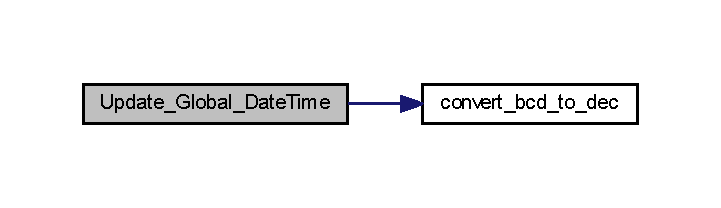
\includegraphics[width=346pt]{a00017_a93b2ace39d0d582b18b136c908d8f092_cgraph}
\end{center}
\end{figure}
Here is the caller graph for this function\+:
\nopagebreak
\begin{figure}[H]
\begin{center}
\leavevmode
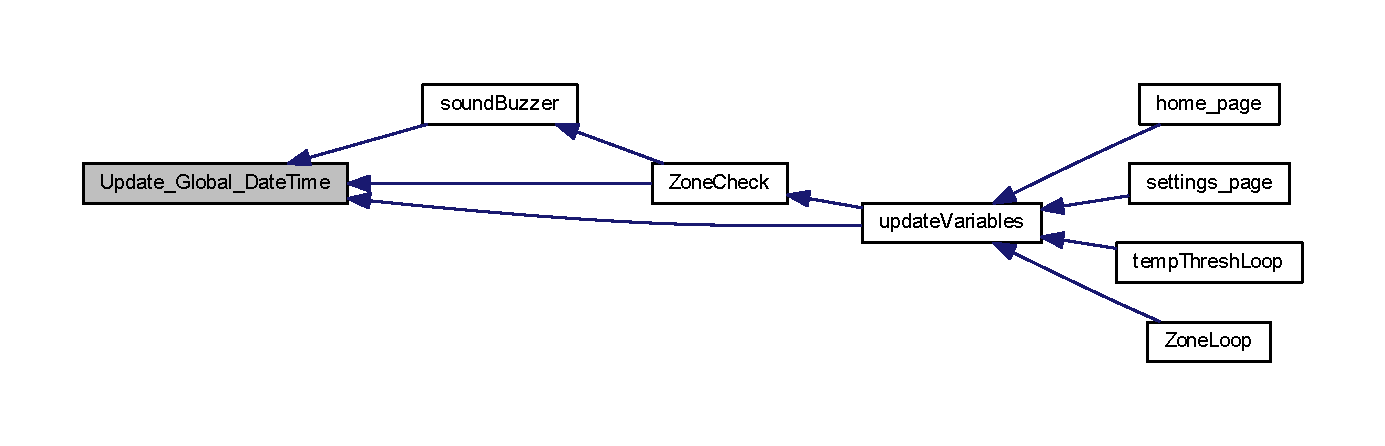
\includegraphics[width=350pt]{a00017_a93b2ace39d0d582b18b136c908d8f092_icgraph}
\end{center}
\end{figure}
\mbox{\label{a00017_a4445924dfb1ef2a828793deff1d6efc0}} 
\index{clock.\+h@{clock.\+h}!Write\+\_\+date\+Time\+\_\+rtc@{Write\+\_\+date\+Time\+\_\+rtc}}
\index{Write\+\_\+date\+Time\+\_\+rtc@{Write\+\_\+date\+Time\+\_\+rtc}!clock.\+h@{clock.\+h}}
\paragraph{Write\+\_\+date\+Time\+\_\+rtc()}
{\footnotesize\ttfamily void Write\+\_\+date\+Time\+\_\+rtc (\begin{DoxyParamCaption}\item[{\textbf{ Date\+Time} $\ast$}]{date }\end{DoxyParamCaption})}

\mbox{\label{a00017_aadecf4eb7d23c63d1216ced71440654e}} 
\index{clock.\+h@{clock.\+h}!write\+\_\+time\+\_\+rtc@{write\+\_\+time\+\_\+rtc}}
\index{write\+\_\+time\+\_\+rtc@{write\+\_\+time\+\_\+rtc}!clock.\+h@{clock.\+h}}
\paragraph{write\+\_\+time\+\_\+rtc()}
{\footnotesize\ttfamily void write\+\_\+time\+\_\+rtc (\begin{DoxyParamCaption}\item[{unsigned char}]{time\+\_\+tx }\end{DoxyParamCaption})}

Here is the caller graph for this function\+:
\nopagebreak
\begin{figure}[H]
\begin{center}
\leavevmode
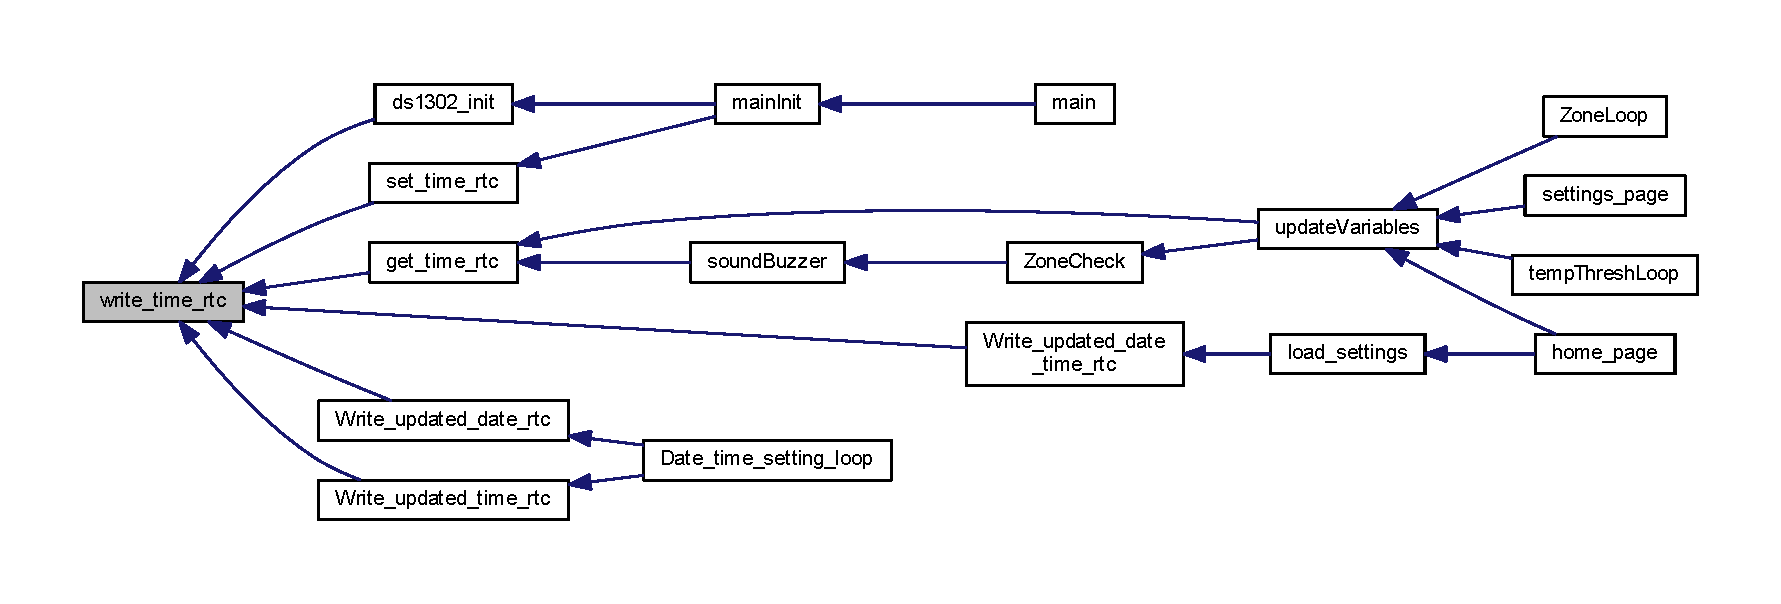
\includegraphics[width=350pt]{a00017_aadecf4eb7d23c63d1216ced71440654e_icgraph}
\end{center}
\end{figure}
\mbox{\label{a00017_a7ae143903216d08d3f0c07b95e21c21b}} 
\index{clock.\+h@{clock.\+h}!Write\+\_\+updated\+\_\+date\+\_\+rtc@{Write\+\_\+updated\+\_\+date\+\_\+rtc}}
\index{Write\+\_\+updated\+\_\+date\+\_\+rtc@{Write\+\_\+updated\+\_\+date\+\_\+rtc}!clock.\+h@{clock.\+h}}
\paragraph{Write\+\_\+updated\+\_\+date\+\_\+rtc()}
{\footnotesize\ttfamily void Write\+\_\+updated\+\_\+date\+\_\+rtc (\begin{DoxyParamCaption}\item[{\textbf{ Date\+Time} $\ast$}]{date }\end{DoxyParamCaption})}

Here is the call graph for this function\+:
\nopagebreak
\begin{figure}[H]
\begin{center}
\leavevmode
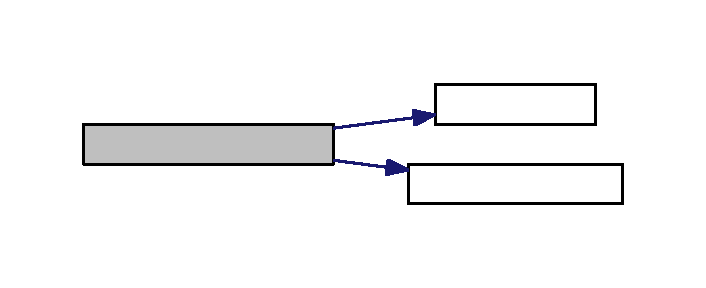
\includegraphics[width=339pt]{a00017_a7ae143903216d08d3f0c07b95e21c21b_cgraph}
\end{center}
\end{figure}
Here is the caller graph for this function\+:
\nopagebreak
\begin{figure}[H]
\begin{center}
\leavevmode
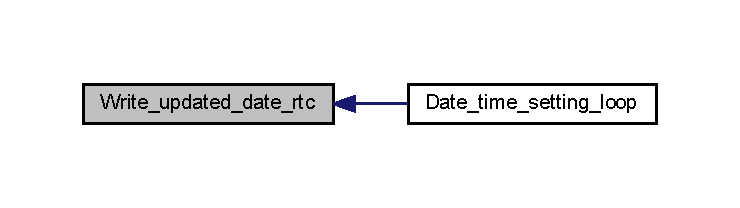
\includegraphics[width=350pt]{a00017_a7ae143903216d08d3f0c07b95e21c21b_icgraph}
\end{center}
\end{figure}
\mbox{\label{a00017_ad20fe32d70b509ba8f7f24a572e34f3f}} 
\index{clock.\+h@{clock.\+h}!Write\+\_\+updated\+\_\+date\+\_\+time\+\_\+rtc@{Write\+\_\+updated\+\_\+date\+\_\+time\+\_\+rtc}}
\index{Write\+\_\+updated\+\_\+date\+\_\+time\+\_\+rtc@{Write\+\_\+updated\+\_\+date\+\_\+time\+\_\+rtc}!clock.\+h@{clock.\+h}}
\paragraph{Write\+\_\+updated\+\_\+date\+\_\+time\+\_\+rtc()}
{\footnotesize\ttfamily void Write\+\_\+updated\+\_\+date\+\_\+time\+\_\+rtc (\begin{DoxyParamCaption}\item[{\textbf{ Date\+Time} $\ast$}]{date }\end{DoxyParamCaption})}

Here is the call graph for this function\+:
\nopagebreak
\begin{figure}[H]
\begin{center}
\leavevmode
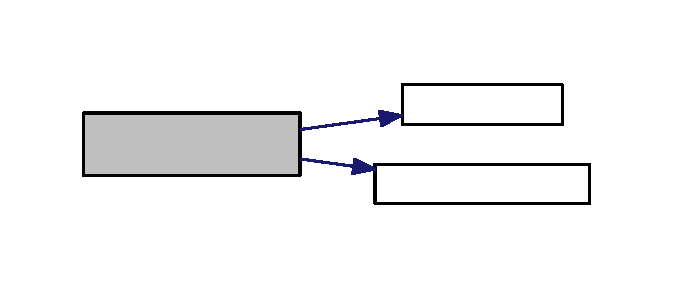
\includegraphics[width=323pt]{a00017_ad20fe32d70b509ba8f7f24a572e34f3f_cgraph}
\end{center}
\end{figure}
Here is the caller graph for this function\+:
\nopagebreak
\begin{figure}[H]
\begin{center}
\leavevmode
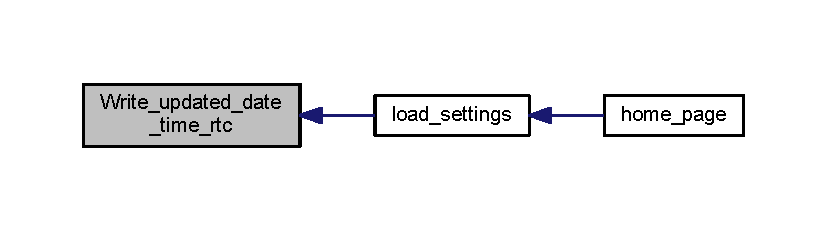
\includegraphics[width=350pt]{a00017_ad20fe32d70b509ba8f7f24a572e34f3f_icgraph}
\end{center}
\end{figure}
\mbox{\label{a00017_a2f6bf3793293cc3f2c09a91c3725a8af}} 
\index{clock.\+h@{clock.\+h}!Write\+\_\+updated\+\_\+time\+\_\+rtc@{Write\+\_\+updated\+\_\+time\+\_\+rtc}}
\index{Write\+\_\+updated\+\_\+time\+\_\+rtc@{Write\+\_\+updated\+\_\+time\+\_\+rtc}!clock.\+h@{clock.\+h}}
\paragraph{Write\+\_\+updated\+\_\+time\+\_\+rtc()}
{\footnotesize\ttfamily void Write\+\_\+updated\+\_\+time\+\_\+rtc (\begin{DoxyParamCaption}\item[{\textbf{ Date\+Time} $\ast$}]{date }\end{DoxyParamCaption})}

Here is the call graph for this function\+:
\nopagebreak
\begin{figure}[H]
\begin{center}
\leavevmode
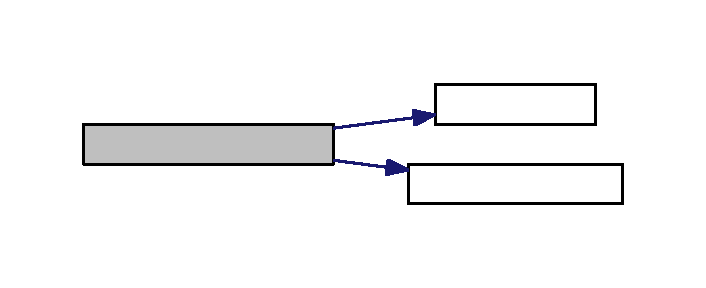
\includegraphics[width=339pt]{a00017_a2f6bf3793293cc3f2c09a91c3725a8af_cgraph}
\end{center}
\end{figure}
Here is the caller graph for this function\+:
\nopagebreak
\begin{figure}[H]
\begin{center}
\leavevmode
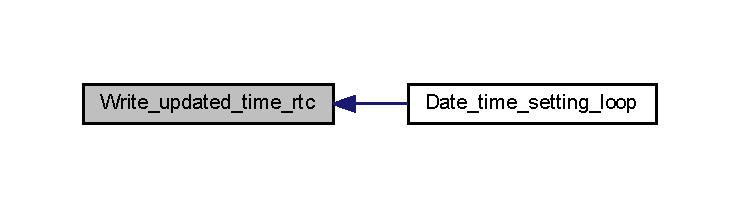
\includegraphics[width=350pt]{a00017_a2f6bf3793293cc3f2c09a91c3725a8af_icgraph}
\end{center}
\end{figure}


\subsubsection{Variable Documentation}
\mbox{\label{a00017_acaf1b7d1c378b3ba535f7989083a8c7e}} 
\index{clock.\+h@{clock.\+h}!Date\+Changed@{Date\+Changed}}
\index{Date\+Changed@{Date\+Changed}!clock.\+h@{clock.\+h}}
\paragraph{Date\+Changed}
{\footnotesize\ttfamily bool Date\+Changed}

\mbox{\label{a00017_a129e222d3019ef1ee0f6a7b86a51ae74}} 
\index{clock.\+h@{clock.\+h}!date\+Time@{date\+Time}}
\index{date\+Time@{date\+Time}!clock.\+h@{clock.\+h}}
\paragraph{date\+Time}
{\footnotesize\ttfamily \textbf{ Date\+Time} date\+Time}

\mbox{\label{a00017_a57e83b1737eee63187e56acce600136c}} 
\index{clock.\+h@{clock.\+h}!rtc\+\_\+7\+\_\+seg\+\_\+display\+\_\+table@{rtc\+\_\+7\+\_\+seg\+\_\+display\+\_\+table}}
\index{rtc\+\_\+7\+\_\+seg\+\_\+display\+\_\+table@{rtc\+\_\+7\+\_\+seg\+\_\+display\+\_\+table}!clock.\+h@{clock.\+h}}
\paragraph{rtc\+\_\+7\+\_\+seg\+\_\+display\+\_\+table}
{\footnotesize\ttfamily const char rtc\+\_\+7\+\_\+seg\+\_\+display\+\_\+table[$\,$] =\{0xc0,0xf9,0xa4,0xb0,0x99,0x92,0x82,0xf8,0x80,0x90\}}

\mbox{\label{a00017_a87a59dfc82addeccd290c9b7e487f2a8}} 
\index{clock.\+h@{clock.\+h}!rtc\+\_\+lcd\+\_\+display\+\_\+date\+\_\+table@{rtc\+\_\+lcd\+\_\+display\+\_\+date\+\_\+table}}
\index{rtc\+\_\+lcd\+\_\+display\+\_\+date\+\_\+table@{rtc\+\_\+lcd\+\_\+display\+\_\+date\+\_\+table}!clock.\+h@{clock.\+h}}
\paragraph{rtc\+\_\+lcd\+\_\+display\+\_\+date\+\_\+table}
{\footnotesize\ttfamily char rtc\+\_\+lcd\+\_\+display\+\_\+date\+\_\+table[9]}

\mbox{\label{a00017_a49d6b1894d5636b2587cfbbfab0eba31}} 
\index{clock.\+h@{clock.\+h}!rtc\+\_\+lcd\+\_\+display\+\_\+time\+\_\+table@{rtc\+\_\+lcd\+\_\+display\+\_\+time\+\_\+table}}
\index{rtc\+\_\+lcd\+\_\+display\+\_\+time\+\_\+table@{rtc\+\_\+lcd\+\_\+display\+\_\+time\+\_\+table}!clock.\+h@{clock.\+h}}
\paragraph{rtc\+\_\+lcd\+\_\+display\+\_\+time\+\_\+table}
{\footnotesize\ttfamily char rtc\+\_\+lcd\+\_\+display\+\_\+time\+\_\+table[9]}

\mbox{\label{a00017_a021cd228e8beae68982b7c03acf5d060}} 
\index{clock.\+h@{clock.\+h}!rtc\+\_\+table@{rtc\+\_\+table}}
\index{rtc\+\_\+table@{rtc\+\_\+table}!clock.\+h@{clock.\+h}}
\paragraph{rtc\+\_\+table}
{\footnotesize\ttfamily const char rtc\+\_\+table[$\,$] =\{0x00, 0x58, 0x12, 0x12, 0x12, 0x06, 0x17, 0x00\}}

\mbox{\label{a00017_a3c5af18aaa8845c69095c105f0ca8997}} 
\index{clock.\+h@{clock.\+h}!rtc\+\_\+table1@{rtc\+\_\+table1}}
\index{rtc\+\_\+table1@{rtc\+\_\+table1}!clock.\+h@{clock.\+h}}
\paragraph{rtc\+\_\+table1}
{\footnotesize\ttfamily char rtc\+\_\+table1[7]}

\mbox{\label{a00017_a878db895116fbbee698e727062540d31}} 
\index{clock.\+h@{clock.\+h}!time\+\_\+rx@{time\+\_\+rx}}
\index{time\+\_\+rx@{time\+\_\+rx}!clock.\+h@{clock.\+h}}
\paragraph{time\+\_\+rx}
{\footnotesize\ttfamily unsigned char time\+\_\+rx}


\subsection{common.\+c File Reference}
\label{a00020}\index{common.\+c@{common.\+c}}
{\ttfamily \#include \char`\"{}Commonheader.\+h\char`\"{}}\newline
Include dependency graph for common.\+c\+:
\nopagebreak
\begin{figure}[H]
\begin{center}
\leavevmode
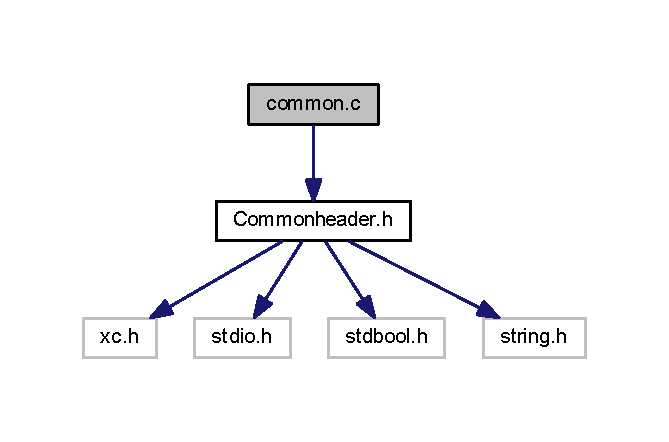
\includegraphics[width=321pt]{a00021}
\end{center}
\end{figure}
\subsubsection*{Functions}
\begin{DoxyCompactItemize}
\item 
void \textbf{ Delay\+\_\+loop} (unsigned long j)
\item 
unsigned char \textbf{ convert\+\_\+from\+\_\+bit\+\_\+pos} (unsigned char bit\+Pos)
\item 
void \textbf{ Clear\+Buttons} ()
\item 
unsigned char \textbf{ convert\+\_\+to\+\_\+bit\+\_\+pos} (unsigned char pin\+Num)
\item 
bool \textbf{ single\+\_\+key\+\_\+pressed} (char byte\+Val)
\item 
\textbf{ Date\+Time} $\ast$ \textbf{ convert\+Date\+From\+Array} (unsigned char input[$\,$])
\item 
void \textbf{ Button\+Init} ()
\item 
unsigned char \textbf{ convert\+\_\+bcd\+\_\+to\+\_\+dec} (unsigned char val)
\item 
unsigned char \textbf{ convert\+\_\+dec\+\_\+to\+\_\+bcd} (unsigned char val)
\end{DoxyCompactItemize}


\subsubsection{Function Documentation}
\mbox{\label{a00020_af645ecef369e812aeddaef421d32fda3}} 
\index{common.\+c@{common.\+c}!Button\+Init@{Button\+Init}}
\index{Button\+Init@{Button\+Init}!common.\+c@{common.\+c}}
\paragraph{Button\+Init()}
{\footnotesize\ttfamily void Button\+Init (\begin{DoxyParamCaption}\item[{void}]{ }\end{DoxyParamCaption})}

Here is the caller graph for this function\+:
\nopagebreak
\begin{figure}[H]
\begin{center}
\leavevmode
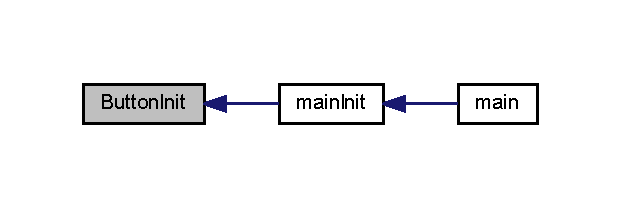
\includegraphics[width=298pt]{a00020_af645ecef369e812aeddaef421d32fda3_icgraph}
\end{center}
\end{figure}
\mbox{\label{a00020_ad54189d97d4ebc2ac5e310be78d7968f}} 
\index{common.\+c@{common.\+c}!Clear\+Buttons@{Clear\+Buttons}}
\index{Clear\+Buttons@{Clear\+Buttons}!common.\+c@{common.\+c}}
\paragraph{Clear\+Buttons()}
{\footnotesize\ttfamily void Clear\+Buttons (\begin{DoxyParamCaption}\item[{void}]{ }\end{DoxyParamCaption})}

Here is the caller graph for this function\+:
\nopagebreak
\begin{figure}[H]
\begin{center}
\leavevmode
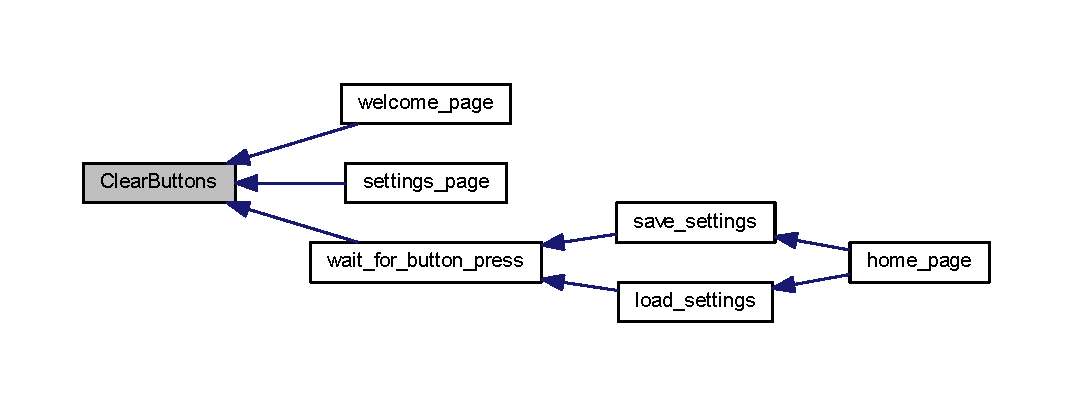
\includegraphics[width=350pt]{a00020_ad54189d97d4ebc2ac5e310be78d7968f_icgraph}
\end{center}
\end{figure}
\mbox{\label{a00020_a03795fe6451769e81af8ef69856e8acb}} 
\index{common.\+c@{common.\+c}!convert\+\_\+bcd\+\_\+to\+\_\+dec@{convert\+\_\+bcd\+\_\+to\+\_\+dec}}
\index{convert\+\_\+bcd\+\_\+to\+\_\+dec@{convert\+\_\+bcd\+\_\+to\+\_\+dec}!common.\+c@{common.\+c}}
\paragraph{convert\+\_\+bcd\+\_\+to\+\_\+dec()}
{\footnotesize\ttfamily unsigned char convert\+\_\+bcd\+\_\+to\+\_\+dec (\begin{DoxyParamCaption}\item[{unsigned char}]{val }\end{DoxyParamCaption})}

Here is the caller graph for this function\+:
\nopagebreak
\begin{figure}[H]
\begin{center}
\leavevmode
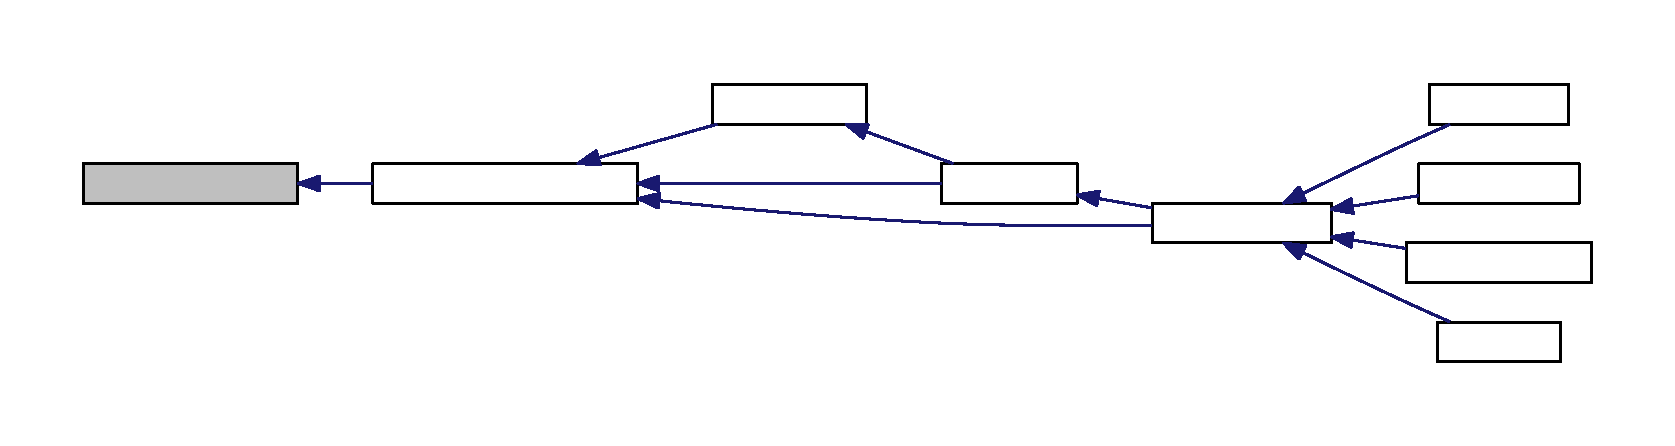
\includegraphics[width=350pt]{a00020_a03795fe6451769e81af8ef69856e8acb_icgraph}
\end{center}
\end{figure}
\mbox{\label{a00020_abaa7c975d4dd864dbf88ce3c10029aa4}} 
\index{common.\+c@{common.\+c}!convert\+\_\+dec\+\_\+to\+\_\+bcd@{convert\+\_\+dec\+\_\+to\+\_\+bcd}}
\index{convert\+\_\+dec\+\_\+to\+\_\+bcd@{convert\+\_\+dec\+\_\+to\+\_\+bcd}!common.\+c@{common.\+c}}
\paragraph{convert\+\_\+dec\+\_\+to\+\_\+bcd()}
{\footnotesize\ttfamily unsigned char convert\+\_\+dec\+\_\+to\+\_\+bcd (\begin{DoxyParamCaption}\item[{unsigned char}]{val }\end{DoxyParamCaption})}

Here is the caller graph for this function\+:
\nopagebreak
\begin{figure}[H]
\begin{center}
\leavevmode
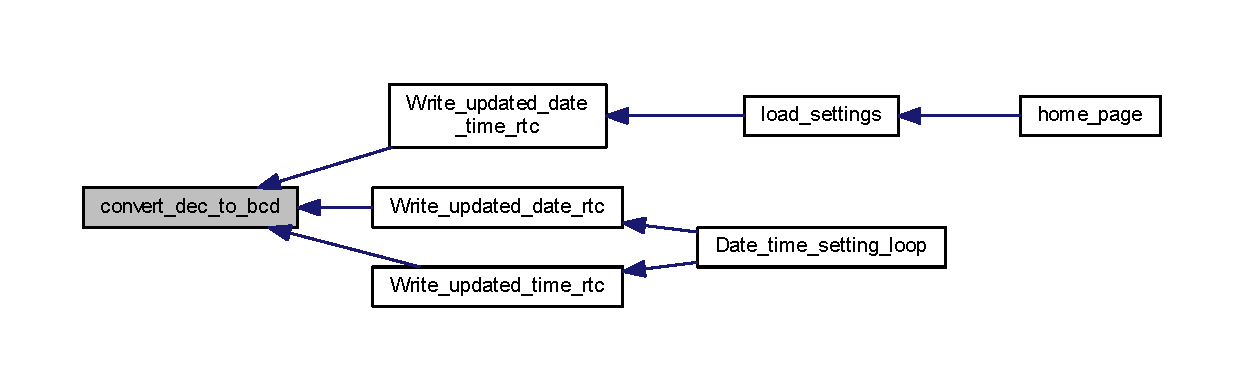
\includegraphics[width=350pt]{a00020_abaa7c975d4dd864dbf88ce3c10029aa4_icgraph}
\end{center}
\end{figure}
\mbox{\label{a00020_a0975bad4a272465d34f2dd42b61929f9}} 
\index{common.\+c@{common.\+c}!convert\+\_\+from\+\_\+bit\+\_\+pos@{convert\+\_\+from\+\_\+bit\+\_\+pos}}
\index{convert\+\_\+from\+\_\+bit\+\_\+pos@{convert\+\_\+from\+\_\+bit\+\_\+pos}!common.\+c@{common.\+c}}
\paragraph{convert\+\_\+from\+\_\+bit\+\_\+pos()}
{\footnotesize\ttfamily unsigned char convert\+\_\+from\+\_\+bit\+\_\+pos (\begin{DoxyParamCaption}\item[{unsigned char}]{bit\+Pos }\end{DoxyParamCaption})}

Here is the caller graph for this function\+:
\nopagebreak
\begin{figure}[H]
\begin{center}
\leavevmode
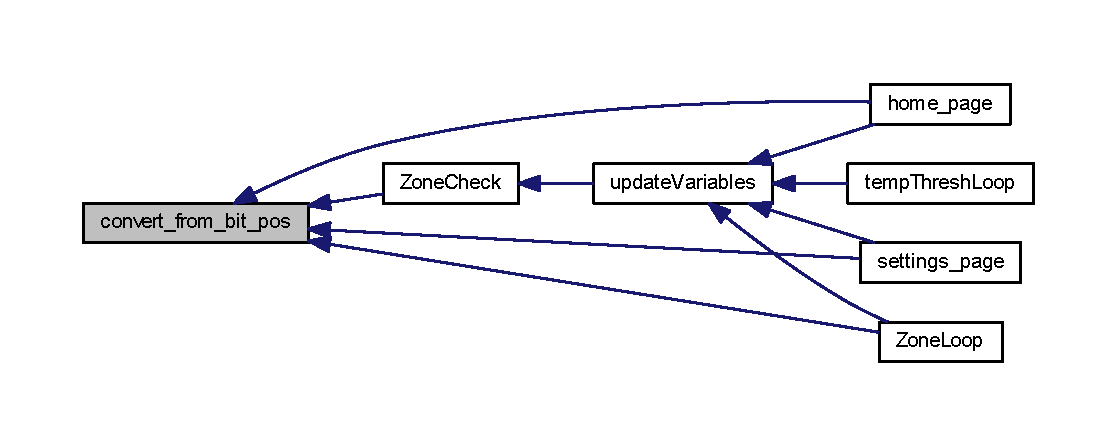
\includegraphics[width=350pt]{a00020_a0975bad4a272465d34f2dd42b61929f9_icgraph}
\end{center}
\end{figure}
\mbox{\label{a00020_ac22561642e81efb7df183503c322c2b0}} 
\index{common.\+c@{common.\+c}!convert\+\_\+to\+\_\+bit\+\_\+pos@{convert\+\_\+to\+\_\+bit\+\_\+pos}}
\index{convert\+\_\+to\+\_\+bit\+\_\+pos@{convert\+\_\+to\+\_\+bit\+\_\+pos}!common.\+c@{common.\+c}}
\paragraph{convert\+\_\+to\+\_\+bit\+\_\+pos()}
{\footnotesize\ttfamily unsigned char convert\+\_\+to\+\_\+bit\+\_\+pos (\begin{DoxyParamCaption}\item[{unsigned char}]{pin\+Num }\end{DoxyParamCaption})}

Here is the caller graph for this function\+:
\nopagebreak
\begin{figure}[H]
\begin{center}
\leavevmode
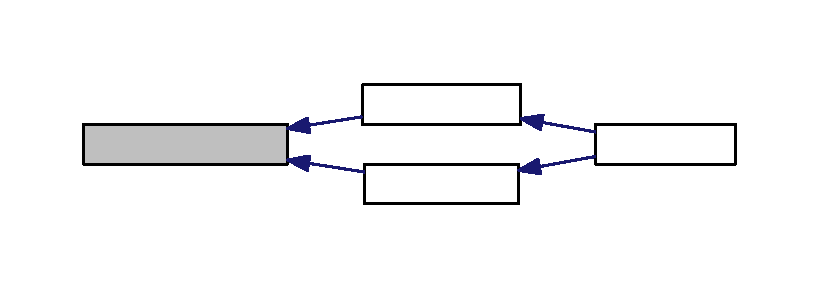
\includegraphics[width=350pt]{a00020_ac22561642e81efb7df183503c322c2b0_icgraph}
\end{center}
\end{figure}
\mbox{\label{a00020_abbe3f18b8a8d4112e5d5f3d1764ccabf}} 
\index{common.\+c@{common.\+c}!convert\+Date\+From\+Array@{convert\+Date\+From\+Array}}
\index{convert\+Date\+From\+Array@{convert\+Date\+From\+Array}!common.\+c@{common.\+c}}
\paragraph{convert\+Date\+From\+Array()}
{\footnotesize\ttfamily \textbf{ Date\+Time}$\ast$ convert\+Date\+From\+Array (\begin{DoxyParamCaption}\item[{unsigned char}]{input[$\,$] }\end{DoxyParamCaption})}

Here is the caller graph for this function\+:
\nopagebreak
\begin{figure}[H]
\begin{center}
\leavevmode
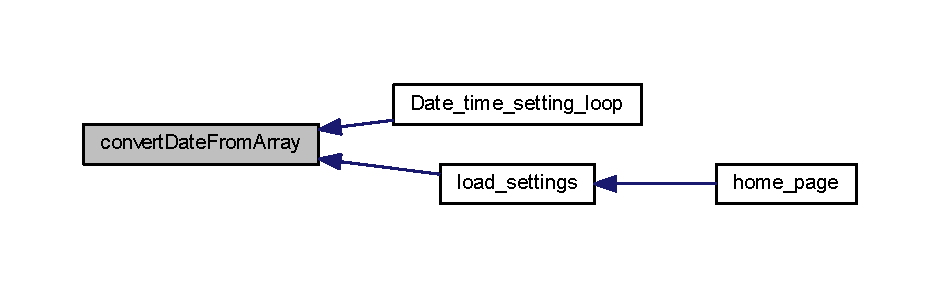
\includegraphics[width=350pt]{a00020_abbe3f18b8a8d4112e5d5f3d1764ccabf_icgraph}
\end{center}
\end{figure}
\mbox{\label{a00020_a4ac586173db65fe258489805cd2a50a7}} 
\index{common.\+c@{common.\+c}!Delay\+\_\+loop@{Delay\+\_\+loop}}
\index{Delay\+\_\+loop@{Delay\+\_\+loop}!common.\+c@{common.\+c}}
\paragraph{Delay\+\_\+loop()}
{\footnotesize\ttfamily void Delay\+\_\+loop (\begin{DoxyParamCaption}\item[{unsigned long}]{j }\end{DoxyParamCaption})}

Here is the caller graph for this function\+:
\nopagebreak
\begin{figure}[H]
\begin{center}
\leavevmode
\includegraphics[width=350pt]{a00020_a4ac586173db65fe258489805cd2a50a7_icgraph}
\end{center}
\end{figure}
\mbox{\label{a00020_a8ac785f2d4c8d133c61c4e9be06cb606}} 
\index{common.\+c@{common.\+c}!single\+\_\+key\+\_\+pressed@{single\+\_\+key\+\_\+pressed}}
\index{single\+\_\+key\+\_\+pressed@{single\+\_\+key\+\_\+pressed}!common.\+c@{common.\+c}}
\paragraph{single\+\_\+key\+\_\+pressed()}
{\footnotesize\ttfamily bool single\+\_\+key\+\_\+pressed (\begin{DoxyParamCaption}\item[{char}]{byte\+Val }\end{DoxyParamCaption})}

Here is the caller graph for this function\+:
\nopagebreak
\begin{figure}[H]
\begin{center}
\leavevmode
\includegraphics[width=350pt]{a00020_a8ac785f2d4c8d133c61c4e9be06cb606_icgraph}
\end{center}
\end{figure}

\subsection{Commonheader.\+h File Reference}
\label{a00023}\index{Commonheader.\+h@{Commonheader.\+h}}
{\ttfamily \#include $<$xc.\+h$>$}\newline
{\ttfamily \#include $<$stdio.\+h$>$}\newline
{\ttfamily \#include $<$stdbool.\+h$>$}\newline
{\ttfamily \#include $<$string.\+h$>$}\newline
Include dependency graph for Commonheader.\+h\+:
\nopagebreak
\begin{figure}[H]
\begin{center}
\leavevmode
\includegraphics[width=321pt]{a00024}
\end{center}
\end{figure}
This graph shows which files directly or indirectly include this file\+:
\nopagebreak
\begin{figure}[H]
\begin{center}
\leavevmode
\includegraphics[width=350pt]{a00025}
\end{center}
\end{figure}
\subsubsection*{Data Structures}
\begin{DoxyCompactItemize}
\item 
struct \textbf{ Date\+Time}
\end{DoxyCompactItemize}
\subsubsection*{Macros}
\begin{DoxyCompactItemize}
\item 
\#define \textbf{ Pin}(n)~(1 $<$$<$ n)
\item 
\#define \textbf{ B\+U\+T\+T\+O\+N\+\_\+\+M\+A\+SK}~0x0F
\item 
\#define \textbf{ I\+N\+C\+R\+E\+M\+E\+NT}~0x01
\item 
\#define \textbf{ D\+E\+C\+R\+E\+M\+E\+NT}~0x02
\item 
\#define \textbf{ M\+O\+V\+E\+\_\+\+R\+I\+G\+HT}~0x04
\item 
\#define \textbf{ M\+O\+V\+E\+\_\+\+L\+E\+FT}~0x08
\end{DoxyCompactItemize}
\subsubsection*{Functions}
\begin{DoxyCompactItemize}
\item 
int \textbf{ Button\+Check} (void)
\item 
void \textbf{ Button\+Init} (void)
\item 
void \textbf{ update\+Variables} (void)
\item 
void \textbf{ Delay\+\_\+loop} (unsigned long j)
\item 
unsigned char \textbf{ convert\+\_\+from\+\_\+bit\+\_\+pos} (unsigned char bit\+Pos)
\item 
unsigned char \textbf{ convert\+\_\+to\+\_\+bit\+\_\+pos} (unsigned char pin\+Num)
\item 
bool \textbf{ single\+\_\+key\+\_\+pressed} (char byte\+Val)
\item 
void \textbf{ Clear\+Buttons} (void)
\item 
unsigned char \textbf{ convert\+\_\+bcd\+\_\+to\+\_\+dec} (unsigned char val)
\item 
unsigned char \textbf{ convert\+\_\+dec\+\_\+to\+\_\+bcd} (unsigned char val)
\item 
\textbf{ Date\+Time} $\ast$ \textbf{ convert\+Date\+From\+Array} (unsigned char input[$\,$])
\end{DoxyCompactItemize}
\subsubsection*{Variables}
\begin{DoxyCompactItemize}
\item 
int \textbf{ prev\+Butt} = -\/1
\item 
unsigned \textbf{ last\+Pressed} = 9
\item 
\textbf{ Date\+Time} \textbf{ date\+Time}
\item 
\textbf{ Date\+Time} \textbf{ alarm\+Duration}
\item 
bool \textbf{ Date\+Changed}
\item 
int \textbf{ current\+\_\+alarm\+\_\+duration}
\item 
bool \textbf{ active\+Zones} [4]
\end{DoxyCompactItemize}


\subsubsection{Macro Definition Documentation}
\mbox{\label{a00023_afe20026ae95d143f6354cd1bb5b7a0a9}} 
\index{Commonheader.\+h@{Commonheader.\+h}!B\+U\+T\+T\+O\+N\+\_\+\+M\+A\+SK@{B\+U\+T\+T\+O\+N\+\_\+\+M\+A\+SK}}
\index{B\+U\+T\+T\+O\+N\+\_\+\+M\+A\+SK@{B\+U\+T\+T\+O\+N\+\_\+\+M\+A\+SK}!Commonheader.\+h@{Commonheader.\+h}}
\paragraph{B\+U\+T\+T\+O\+N\+\_\+\+M\+A\+SK}
{\footnotesize\ttfamily \#define B\+U\+T\+T\+O\+N\+\_\+\+M\+A\+SK~0x0F}

\mbox{\label{a00023_a922175f7c5b47ad6cdfdb2dca80b5648}} 
\index{Commonheader.\+h@{Commonheader.\+h}!D\+E\+C\+R\+E\+M\+E\+NT@{D\+E\+C\+R\+E\+M\+E\+NT}}
\index{D\+E\+C\+R\+E\+M\+E\+NT@{D\+E\+C\+R\+E\+M\+E\+NT}!Commonheader.\+h@{Commonheader.\+h}}
\paragraph{D\+E\+C\+R\+E\+M\+E\+NT}
{\footnotesize\ttfamily \#define D\+E\+C\+R\+E\+M\+E\+NT~0x02}

\mbox{\label{a00023_ad99a3089c13b6f47b26b218a997fad73}} 
\index{Commonheader.\+h@{Commonheader.\+h}!I\+N\+C\+R\+E\+M\+E\+NT@{I\+N\+C\+R\+E\+M\+E\+NT}}
\index{I\+N\+C\+R\+E\+M\+E\+NT@{I\+N\+C\+R\+E\+M\+E\+NT}!Commonheader.\+h@{Commonheader.\+h}}
\paragraph{I\+N\+C\+R\+E\+M\+E\+NT}
{\footnotesize\ttfamily \#define I\+N\+C\+R\+E\+M\+E\+NT~0x01}

\mbox{\label{a00023_a4796d02bb619233fee554b3ff9c8da48}} 
\index{Commonheader.\+h@{Commonheader.\+h}!M\+O\+V\+E\+\_\+\+L\+E\+FT@{M\+O\+V\+E\+\_\+\+L\+E\+FT}}
\index{M\+O\+V\+E\+\_\+\+L\+E\+FT@{M\+O\+V\+E\+\_\+\+L\+E\+FT}!Commonheader.\+h@{Commonheader.\+h}}
\paragraph{M\+O\+V\+E\+\_\+\+L\+E\+FT}
{\footnotesize\ttfamily \#define M\+O\+V\+E\+\_\+\+L\+E\+FT~0x08}

\mbox{\label{a00023_a001bb501c43a2caa67dc0d3245bd073c}} 
\index{Commonheader.\+h@{Commonheader.\+h}!M\+O\+V\+E\+\_\+\+R\+I\+G\+HT@{M\+O\+V\+E\+\_\+\+R\+I\+G\+HT}}
\index{M\+O\+V\+E\+\_\+\+R\+I\+G\+HT@{M\+O\+V\+E\+\_\+\+R\+I\+G\+HT}!Commonheader.\+h@{Commonheader.\+h}}
\paragraph{M\+O\+V\+E\+\_\+\+R\+I\+G\+HT}
{\footnotesize\ttfamily \#define M\+O\+V\+E\+\_\+\+R\+I\+G\+HT~0x04}

\mbox{\label{a00023_a11259431994827b5ec3f33b36d6d0a2e}} 
\index{Commonheader.\+h@{Commonheader.\+h}!Pin@{Pin}}
\index{Pin@{Pin}!Commonheader.\+h@{Commonheader.\+h}}
\paragraph{Pin}
{\footnotesize\ttfamily \#define Pin(\begin{DoxyParamCaption}\item[{}]{n }\end{DoxyParamCaption})~(1 $<$$<$ n)}



\subsubsection{Function Documentation}
\mbox{\label{a00023_a0bcbbfbc2b8750738cfd3bd92caac260}} 
\index{Commonheader.\+h@{Commonheader.\+h}!Button\+Check@{Button\+Check}}
\index{Button\+Check@{Button\+Check}!Commonheader.\+h@{Commonheader.\+h}}
\paragraph{Button\+Check()}
{\footnotesize\ttfamily int Button\+Check (\begin{DoxyParamCaption}\item[{void}]{ }\end{DoxyParamCaption})}

\mbox{\label{a00023_a30a1cff81be3c91e307685387401e863}} 
\index{Commonheader.\+h@{Commonheader.\+h}!Button\+Init@{Button\+Init}}
\index{Button\+Init@{Button\+Init}!Commonheader.\+h@{Commonheader.\+h}}
\paragraph{Button\+Init()}
{\footnotesize\ttfamily void Button\+Init (\begin{DoxyParamCaption}\item[{void}]{ }\end{DoxyParamCaption})}

Here is the caller graph for this function\+:
\nopagebreak
\begin{figure}[H]
\begin{center}
\leavevmode
\includegraphics[width=298pt]{a00023_a30a1cff81be3c91e307685387401e863_icgraph}
\end{center}
\end{figure}
\mbox{\label{a00023_a034e39ae5657bf5b846d4ce5ff0a6047}} 
\index{Commonheader.\+h@{Commonheader.\+h}!Clear\+Buttons@{Clear\+Buttons}}
\index{Clear\+Buttons@{Clear\+Buttons}!Commonheader.\+h@{Commonheader.\+h}}
\paragraph{Clear\+Buttons()}
{\footnotesize\ttfamily void Clear\+Buttons (\begin{DoxyParamCaption}\item[{void}]{ }\end{DoxyParamCaption})}

Here is the caller graph for this function\+:
\nopagebreak
\begin{figure}[H]
\begin{center}
\leavevmode
\includegraphics[width=350pt]{a00023_a034e39ae5657bf5b846d4ce5ff0a6047_icgraph}
\end{center}
\end{figure}
\mbox{\label{a00023_a03795fe6451769e81af8ef69856e8acb}} 
\index{Commonheader.\+h@{Commonheader.\+h}!convert\+\_\+bcd\+\_\+to\+\_\+dec@{convert\+\_\+bcd\+\_\+to\+\_\+dec}}
\index{convert\+\_\+bcd\+\_\+to\+\_\+dec@{convert\+\_\+bcd\+\_\+to\+\_\+dec}!Commonheader.\+h@{Commonheader.\+h}}
\paragraph{convert\+\_\+bcd\+\_\+to\+\_\+dec()}
{\footnotesize\ttfamily unsigned char convert\+\_\+bcd\+\_\+to\+\_\+dec (\begin{DoxyParamCaption}\item[{unsigned char}]{val }\end{DoxyParamCaption})}

Here is the caller graph for this function\+:
\nopagebreak
\begin{figure}[H]
\begin{center}
\leavevmode
\includegraphics[width=350pt]{a00023_a03795fe6451769e81af8ef69856e8acb_icgraph}
\end{center}
\end{figure}
\mbox{\label{a00023_abaa7c975d4dd864dbf88ce3c10029aa4}} 
\index{Commonheader.\+h@{Commonheader.\+h}!convert\+\_\+dec\+\_\+to\+\_\+bcd@{convert\+\_\+dec\+\_\+to\+\_\+bcd}}
\index{convert\+\_\+dec\+\_\+to\+\_\+bcd@{convert\+\_\+dec\+\_\+to\+\_\+bcd}!Commonheader.\+h@{Commonheader.\+h}}
\paragraph{convert\+\_\+dec\+\_\+to\+\_\+bcd()}
{\footnotesize\ttfamily unsigned char convert\+\_\+dec\+\_\+to\+\_\+bcd (\begin{DoxyParamCaption}\item[{unsigned char}]{val }\end{DoxyParamCaption})}

Here is the caller graph for this function\+:
\nopagebreak
\begin{figure}[H]
\begin{center}
\leavevmode
\includegraphics[width=350pt]{a00023_abaa7c975d4dd864dbf88ce3c10029aa4_icgraph}
\end{center}
\end{figure}
\mbox{\label{a00023_a0975bad4a272465d34f2dd42b61929f9}} 
\index{Commonheader.\+h@{Commonheader.\+h}!convert\+\_\+from\+\_\+bit\+\_\+pos@{convert\+\_\+from\+\_\+bit\+\_\+pos}}
\index{convert\+\_\+from\+\_\+bit\+\_\+pos@{convert\+\_\+from\+\_\+bit\+\_\+pos}!Commonheader.\+h@{Commonheader.\+h}}
\paragraph{convert\+\_\+from\+\_\+bit\+\_\+pos()}
{\footnotesize\ttfamily unsigned char convert\+\_\+from\+\_\+bit\+\_\+pos (\begin{DoxyParamCaption}\item[{unsigned char}]{bit\+Pos }\end{DoxyParamCaption})}

Here is the caller graph for this function\+:
\nopagebreak
\begin{figure}[H]
\begin{center}
\leavevmode
\includegraphics[width=350pt]{a00023_a0975bad4a272465d34f2dd42b61929f9_icgraph}
\end{center}
\end{figure}
\mbox{\label{a00023_ac22561642e81efb7df183503c322c2b0}} 
\index{Commonheader.\+h@{Commonheader.\+h}!convert\+\_\+to\+\_\+bit\+\_\+pos@{convert\+\_\+to\+\_\+bit\+\_\+pos}}
\index{convert\+\_\+to\+\_\+bit\+\_\+pos@{convert\+\_\+to\+\_\+bit\+\_\+pos}!Commonheader.\+h@{Commonheader.\+h}}
\paragraph{convert\+\_\+to\+\_\+bit\+\_\+pos()}
{\footnotesize\ttfamily unsigned char convert\+\_\+to\+\_\+bit\+\_\+pos (\begin{DoxyParamCaption}\item[{unsigned char}]{pin\+Num }\end{DoxyParamCaption})}

Here is the caller graph for this function\+:
\nopagebreak
\begin{figure}[H]
\begin{center}
\leavevmode
\includegraphics[width=350pt]{a00023_ac22561642e81efb7df183503c322c2b0_icgraph}
\end{center}
\end{figure}
\mbox{\label{a00023_abbe3f18b8a8d4112e5d5f3d1764ccabf}} 
\index{Commonheader.\+h@{Commonheader.\+h}!convert\+Date\+From\+Array@{convert\+Date\+From\+Array}}
\index{convert\+Date\+From\+Array@{convert\+Date\+From\+Array}!Commonheader.\+h@{Commonheader.\+h}}
\paragraph{convert\+Date\+From\+Array()}
{\footnotesize\ttfamily \textbf{ Date\+Time}$\ast$ convert\+Date\+From\+Array (\begin{DoxyParamCaption}\item[{unsigned char}]{input[$\,$] }\end{DoxyParamCaption})}

Here is the caller graph for this function\+:
\nopagebreak
\begin{figure}[H]
\begin{center}
\leavevmode
\includegraphics[width=350pt]{a00023_abbe3f18b8a8d4112e5d5f3d1764ccabf_icgraph}
\end{center}
\end{figure}
\mbox{\label{a00023_a4ac586173db65fe258489805cd2a50a7}} 
\index{Commonheader.\+h@{Commonheader.\+h}!Delay\+\_\+loop@{Delay\+\_\+loop}}
\index{Delay\+\_\+loop@{Delay\+\_\+loop}!Commonheader.\+h@{Commonheader.\+h}}
\paragraph{Delay\+\_\+loop()}
{\footnotesize\ttfamily void Delay\+\_\+loop (\begin{DoxyParamCaption}\item[{unsigned long}]{j }\end{DoxyParamCaption})}

Here is the caller graph for this function\+:
\nopagebreak
\begin{figure}[H]
\begin{center}
\leavevmode
\includegraphics[width=350pt]{a00023_a4ac586173db65fe258489805cd2a50a7_icgraph}
\end{center}
\end{figure}
\mbox{\label{a00023_a8ac785f2d4c8d133c61c4e9be06cb606}} 
\index{Commonheader.\+h@{Commonheader.\+h}!single\+\_\+key\+\_\+pressed@{single\+\_\+key\+\_\+pressed}}
\index{single\+\_\+key\+\_\+pressed@{single\+\_\+key\+\_\+pressed}!Commonheader.\+h@{Commonheader.\+h}}
\paragraph{single\+\_\+key\+\_\+pressed()}
{\footnotesize\ttfamily bool single\+\_\+key\+\_\+pressed (\begin{DoxyParamCaption}\item[{char}]{byte\+Val }\end{DoxyParamCaption})}

Here is the caller graph for this function\+:
\nopagebreak
\begin{figure}[H]
\begin{center}
\leavevmode
\includegraphics[width=350pt]{a00023_a8ac785f2d4c8d133c61c4e9be06cb606_icgraph}
\end{center}
\end{figure}
\mbox{\label{a00023_a77a749cc64c8c52f24cfa7d5a886435e}} 
\index{Commonheader.\+h@{Commonheader.\+h}!update\+Variables@{update\+Variables}}
\index{update\+Variables@{update\+Variables}!Commonheader.\+h@{Commonheader.\+h}}
\paragraph{update\+Variables()}
{\footnotesize\ttfamily void update\+Variables (\begin{DoxyParamCaption}\item[{void}]{ }\end{DoxyParamCaption})}

Here is the call graph for this function\+:
\nopagebreak
\begin{figure}[H]
\begin{center}
\leavevmode
\includegraphics[width=350pt]{a00023_a77a749cc64c8c52f24cfa7d5a886435e_cgraph}
\end{center}
\end{figure}
Here is the caller graph for this function\+:
\nopagebreak
\begin{figure}[H]
\begin{center}
\leavevmode
\includegraphics[width=291pt]{a00023_a77a749cc64c8c52f24cfa7d5a886435e_icgraph}
\end{center}
\end{figure}


\subsubsection{Variable Documentation}
\mbox{\label{a00023_a0c777c89cc8b06ddc6c0176f2c31033f}} 
\index{Commonheader.\+h@{Commonheader.\+h}!active\+Zones@{active\+Zones}}
\index{active\+Zones@{active\+Zones}!Commonheader.\+h@{Commonheader.\+h}}
\paragraph{active\+Zones}
{\footnotesize\ttfamily bool active\+Zones[4]}

\mbox{\label{a00023_a01c2a28170e998893c6428276cb87ae2}} 
\index{Commonheader.\+h@{Commonheader.\+h}!alarm\+Duration@{alarm\+Duration}}
\index{alarm\+Duration@{alarm\+Duration}!Commonheader.\+h@{Commonheader.\+h}}
\paragraph{alarm\+Duration}
{\footnotesize\ttfamily \textbf{ Date\+Time} alarm\+Duration}

\mbox{\label{a00023_ab073eeb8d5a2147ef91fab51d73ab4b2}} 
\index{Commonheader.\+h@{Commonheader.\+h}!current\+\_\+alarm\+\_\+duration@{current\+\_\+alarm\+\_\+duration}}
\index{current\+\_\+alarm\+\_\+duration@{current\+\_\+alarm\+\_\+duration}!Commonheader.\+h@{Commonheader.\+h}}
\paragraph{current\+\_\+alarm\+\_\+duration}
{\footnotesize\ttfamily int current\+\_\+alarm\+\_\+duration}

\mbox{\label{a00023_acaf1b7d1c378b3ba535f7989083a8c7e}} 
\index{Commonheader.\+h@{Commonheader.\+h}!Date\+Changed@{Date\+Changed}}
\index{Date\+Changed@{Date\+Changed}!Commonheader.\+h@{Commonheader.\+h}}
\paragraph{Date\+Changed}
{\footnotesize\ttfamily bool Date\+Changed}

\mbox{\label{a00023_a129e222d3019ef1ee0f6a7b86a51ae74}} 
\index{Commonheader.\+h@{Commonheader.\+h}!date\+Time@{date\+Time}}
\index{date\+Time@{date\+Time}!Commonheader.\+h@{Commonheader.\+h}}
\paragraph{date\+Time}
{\footnotesize\ttfamily \textbf{ Date\+Time} date\+Time}

\mbox{\label{a00023_a4fed233d61569dfeb6c0673b30edb19b}} 
\index{Commonheader.\+h@{Commonheader.\+h}!last\+Pressed@{last\+Pressed}}
\index{last\+Pressed@{last\+Pressed}!Commonheader.\+h@{Commonheader.\+h}}
\paragraph{last\+Pressed}
{\footnotesize\ttfamily unsigned last\+Pressed = 9}

\mbox{\label{a00023_ad1c7b1431d808919a1d6929901e260d5}} 
\index{Commonheader.\+h@{Commonheader.\+h}!prev\+Butt@{prev\+Butt}}
\index{prev\+Butt@{prev\+Butt}!Commonheader.\+h@{Commonheader.\+h}}
\paragraph{prev\+Butt}
{\footnotesize\ttfamily int prev\+Butt = -\/1}


\subsection{date\+\_\+setting.\+c File Reference}
\label{a00026}\index{date\+\_\+setting.\+c@{date\+\_\+setting.\+c}}
{\ttfamily \#include \char`\"{}date\+\_\+setting.\+h\char`\"{}}\newline
Include dependency graph for date\+\_\+setting.\+c\+:
\nopagebreak
\begin{figure}[H]
\begin{center}
\leavevmode
\includegraphics[width=321pt]{a00027}
\end{center}
\end{figure}
\subsubsection*{Macros}
\begin{DoxyCompactItemize}
\item 
\#define \textbf{ D\+A\+T\+E\+\_\+\+O\+F\+F\+S\+ET}~0
\item 
\#define \textbf{ T\+I\+M\+E\+\_\+\+O\+F\+F\+S\+ET}~2
\item 
\#define \textbf{ L\+E\+F\+T\+\_\+\+B\+U\+T\+T\+O\+NS}~P\+O\+R\+TE
\item 
\#define \textbf{ R\+I\+G\+H\+T\+\_\+\+B\+U\+T\+T\+O\+NS}~P\+O\+R\+TB
\item 
\#define \textbf{ D\+AY}~0
\item 
\#define \textbf{ M\+O\+N\+TH}~1
\item 
\#define \textbf{ Y\+E\+AR}~2
\item 
\#define \textbf{ H\+O\+UR}~3
\item 
\#define \textbf{ M\+I\+N\+U\+TE}~4
\item 
\#define \textbf{ S\+E\+C\+O\+ND}~5
\end{DoxyCompactItemize}
\subsubsection*{Typedefs}
\begin{DoxyCompactItemize}
\item 
typedef void($\ast$ \textbf{ display\+\_\+function}) (\textbf{ Date\+Time} \textbf{ date}, int line\+No)
\end{DoxyCompactItemize}
\subsubsection*{Enumerations}
\begin{DoxyCompactItemize}
\item 
enum \textbf{ Date\+Time\+Setting\+State} \{ \textbf{ D\+A\+TE}, 
\textbf{ T\+I\+ME}, 
\textbf{ O\+V\+E\+R\+V\+I\+EW}
 \}
\end{DoxyCompactItemize}
\subsubsection*{Functions}
\begin{DoxyCompactItemize}
\item 
void \textbf{ set\+\_\+leap\+\_\+year\+\_\+status} ()
\item 
void \textbf{ Init} ()
\item 
void \textbf{ Right\+\_\+buttons} ()
\item 
void \textbf{ Date\+\_\+time\+\_\+setting\+\_\+loop} ()
\end{DoxyCompactItemize}
\subsubsection*{Variables}
\begin{DoxyCompactItemize}
\item 
\textbf{ Date\+Time\+Setting\+State} \textbf{ current\+D\+Tstate}
\item 
\textbf{ display\+\_\+function} \textbf{ write\+\_\+functions} [2] = \{\textbf{ Write\+\_\+\+Date\+\_\+\+Settings}, \textbf{ Write\+\_\+\+Time\+\_\+\+Settings}\}
\item 
bool \textbf{ quit}
\item 
bool \textbf{ date\+\_\+changed}
\item 
bool \textbf{ line\+\_\+changed}
\item 
bool \textbf{ new\+\_\+date\+\_\+time\+\_\+set}
\item 
bool \textbf{ leap\+\_\+set}
\item 
bool \textbf{ month\+\_\+changed}
\item 
int \textbf{ count} = 0
\item 
int \textbf{ line} = 0
\item 
int \textbf{ cursor\+\_\+position} = 0x48
\item 
\textbf{ Date\+Time} \textbf{ new\+Date}
\item 
int \textbf{ days\+\_\+per\+\_\+month} [12] = \{31, 28, 31, 30, 31, 30, 31, 31, 30, 31, 30, 31\}
\item 
char \textbf{ title} [15]
\item 
unsigned char \textbf{ command}
\item 
unsigned char \textbf{ sec}
\item 
char \textbf{ date} [6]
\item 
int \textbf{ year}
\end{DoxyCompactItemize}


\subsubsection{Macro Definition Documentation}
\mbox{\label{a00026_a4902403b9625ad0ff39668861e9d0b8e}} 
\index{date\+\_\+setting.\+c@{date\+\_\+setting.\+c}!D\+A\+T\+E\+\_\+\+O\+F\+F\+S\+ET@{D\+A\+T\+E\+\_\+\+O\+F\+F\+S\+ET}}
\index{D\+A\+T\+E\+\_\+\+O\+F\+F\+S\+ET@{D\+A\+T\+E\+\_\+\+O\+F\+F\+S\+ET}!date\+\_\+setting.\+c@{date\+\_\+setting.\+c}}
\paragraph{D\+A\+T\+E\+\_\+\+O\+F\+F\+S\+ET}
{\footnotesize\ttfamily \#define D\+A\+T\+E\+\_\+\+O\+F\+F\+S\+ET~0}

\mbox{\label{a00026_a509a01c55cbe47386fe24602b7c7fda1}} 
\index{date\+\_\+setting.\+c@{date\+\_\+setting.\+c}!D\+AY@{D\+AY}}
\index{D\+AY@{D\+AY}!date\+\_\+setting.\+c@{date\+\_\+setting.\+c}}
\paragraph{D\+AY}
{\footnotesize\ttfamily \#define D\+AY~0}

\mbox{\label{a00026_a4698ae12cf6a8acb5886fffd0ec897e6}} 
\index{date\+\_\+setting.\+c@{date\+\_\+setting.\+c}!H\+O\+UR@{H\+O\+UR}}
\index{H\+O\+UR@{H\+O\+UR}!date\+\_\+setting.\+c@{date\+\_\+setting.\+c}}
\paragraph{H\+O\+UR}
{\footnotesize\ttfamily \#define H\+O\+UR~3}

\mbox{\label{a00026_a9b885de9f143efd0c862ceb054256536}} 
\index{date\+\_\+setting.\+c@{date\+\_\+setting.\+c}!L\+E\+F\+T\+\_\+\+B\+U\+T\+T\+O\+NS@{L\+E\+F\+T\+\_\+\+B\+U\+T\+T\+O\+NS}}
\index{L\+E\+F\+T\+\_\+\+B\+U\+T\+T\+O\+NS@{L\+E\+F\+T\+\_\+\+B\+U\+T\+T\+O\+NS}!date\+\_\+setting.\+c@{date\+\_\+setting.\+c}}
\paragraph{L\+E\+F\+T\+\_\+\+B\+U\+T\+T\+O\+NS}
{\footnotesize\ttfamily \#define L\+E\+F\+T\+\_\+\+B\+U\+T\+T\+O\+NS~P\+O\+R\+TE}

\mbox{\label{a00026_ac1454fa04f41c693f39425697a137d82}} 
\index{date\+\_\+setting.\+c@{date\+\_\+setting.\+c}!M\+I\+N\+U\+TE@{M\+I\+N\+U\+TE}}
\index{M\+I\+N\+U\+TE@{M\+I\+N\+U\+TE}!date\+\_\+setting.\+c@{date\+\_\+setting.\+c}}
\paragraph{M\+I\+N\+U\+TE}
{\footnotesize\ttfamily \#define M\+I\+N\+U\+TE~4}

\mbox{\label{a00026_a3729d06495d9713592f79f3122c9e677}} 
\index{date\+\_\+setting.\+c@{date\+\_\+setting.\+c}!M\+O\+N\+TH@{M\+O\+N\+TH}}
\index{M\+O\+N\+TH@{M\+O\+N\+TH}!date\+\_\+setting.\+c@{date\+\_\+setting.\+c}}
\paragraph{M\+O\+N\+TH}
{\footnotesize\ttfamily \#define M\+O\+N\+TH~1}

\mbox{\label{a00026_a68881b6085c880930037b20764fe5aee}} 
\index{date\+\_\+setting.\+c@{date\+\_\+setting.\+c}!R\+I\+G\+H\+T\+\_\+\+B\+U\+T\+T\+O\+NS@{R\+I\+G\+H\+T\+\_\+\+B\+U\+T\+T\+O\+NS}}
\index{R\+I\+G\+H\+T\+\_\+\+B\+U\+T\+T\+O\+NS@{R\+I\+G\+H\+T\+\_\+\+B\+U\+T\+T\+O\+NS}!date\+\_\+setting.\+c@{date\+\_\+setting.\+c}}
\paragraph{R\+I\+G\+H\+T\+\_\+\+B\+U\+T\+T\+O\+NS}
{\footnotesize\ttfamily \#define R\+I\+G\+H\+T\+\_\+\+B\+U\+T\+T\+O\+NS~P\+O\+R\+TB}

\mbox{\label{a00026_a94212be2394d2d37d9dfd33d07d82dba}} 
\index{date\+\_\+setting.\+c@{date\+\_\+setting.\+c}!S\+E\+C\+O\+ND@{S\+E\+C\+O\+ND}}
\index{S\+E\+C\+O\+ND@{S\+E\+C\+O\+ND}!date\+\_\+setting.\+c@{date\+\_\+setting.\+c}}
\paragraph{S\+E\+C\+O\+ND}
{\footnotesize\ttfamily \#define S\+E\+C\+O\+ND~5}

\mbox{\label{a00026_af575bc8343fa3a770ab179a56be676da}} 
\index{date\+\_\+setting.\+c@{date\+\_\+setting.\+c}!T\+I\+M\+E\+\_\+\+O\+F\+F\+S\+ET@{T\+I\+M\+E\+\_\+\+O\+F\+F\+S\+ET}}
\index{T\+I\+M\+E\+\_\+\+O\+F\+F\+S\+ET@{T\+I\+M\+E\+\_\+\+O\+F\+F\+S\+ET}!date\+\_\+setting.\+c@{date\+\_\+setting.\+c}}
\paragraph{T\+I\+M\+E\+\_\+\+O\+F\+F\+S\+ET}
{\footnotesize\ttfamily \#define T\+I\+M\+E\+\_\+\+O\+F\+F\+S\+ET~2}

\mbox{\label{a00026_a5871356500f559add06ea81d60331b1b}} 
\index{date\+\_\+setting.\+c@{date\+\_\+setting.\+c}!Y\+E\+AR@{Y\+E\+AR}}
\index{Y\+E\+AR@{Y\+E\+AR}!date\+\_\+setting.\+c@{date\+\_\+setting.\+c}}
\paragraph{Y\+E\+AR}
{\footnotesize\ttfamily \#define Y\+E\+AR~2}



\subsubsection{Typedef Documentation}
\mbox{\label{a00026_a6ebd6f799e81d74b1234de4b4512a53b}} 
\index{date\+\_\+setting.\+c@{date\+\_\+setting.\+c}!display\+\_\+function@{display\+\_\+function}}
\index{display\+\_\+function@{display\+\_\+function}!date\+\_\+setting.\+c@{date\+\_\+setting.\+c}}
\paragraph{display\+\_\+function}
{\footnotesize\ttfamily typedef void($\ast$ display\+\_\+function) (\textbf{ Date\+Time} \textbf{ date}, int line\+No)}



\subsubsection{Enumeration Type Documentation}
\mbox{\label{a00026_ac5dae8cd38301984200b2b9615bb3fe5}} 
\index{date\+\_\+setting.\+c@{date\+\_\+setting.\+c}!Date\+Time\+Setting\+State@{Date\+Time\+Setting\+State}}
\index{Date\+Time\+Setting\+State@{Date\+Time\+Setting\+State}!date\+\_\+setting.\+c@{date\+\_\+setting.\+c}}
\paragraph{Date\+Time\+Setting\+State}
{\footnotesize\ttfamily enum \textbf{ Date\+Time\+Setting\+State}}

\begin{DoxyEnumFields}{Enumerator}
\raisebox{\heightof{T}}[0pt][0pt]{\index{D\+A\+TE@{D\+A\+TE}!date\+\_\+setting.\+c@{date\+\_\+setting.\+c}}\index{date\+\_\+setting.\+c@{date\+\_\+setting.\+c}!D\+A\+TE@{D\+A\+TE}}}\mbox{\label{a00026_ac5dae8cd38301984200b2b9615bb3fe5a0ace72efd9e987dfd807365d0ca50141}} 
D\+A\+TE&\\
\hline

\raisebox{\heightof{T}}[0pt][0pt]{\index{T\+I\+ME@{T\+I\+ME}!date\+\_\+setting.\+c@{date\+\_\+setting.\+c}}\index{date\+\_\+setting.\+c@{date\+\_\+setting.\+c}!T\+I\+ME@{T\+I\+ME}}}\mbox{\label{a00026_ac5dae8cd38301984200b2b9615bb3fe5ae9e4c627760f36823cdd153c24229157}} 
T\+I\+ME&\\
\hline

\raisebox{\heightof{T}}[0pt][0pt]{\index{O\+V\+E\+R\+V\+I\+EW@{O\+V\+E\+R\+V\+I\+EW}!date\+\_\+setting.\+c@{date\+\_\+setting.\+c}}\index{date\+\_\+setting.\+c@{date\+\_\+setting.\+c}!O\+V\+E\+R\+V\+I\+EW@{O\+V\+E\+R\+V\+I\+EW}}}\mbox{\label{a00026_ac5dae8cd38301984200b2b9615bb3fe5ab1eb7a6917170ab35f0a2b74982419fc}} 
O\+V\+E\+R\+V\+I\+EW&\\
\hline

\end{DoxyEnumFields}


\subsubsection{Function Documentation}
\mbox{\label{a00026_a9dc57df410d5474edcc75f449aa0b960}} 
\index{date\+\_\+setting.\+c@{date\+\_\+setting.\+c}!Date\+\_\+time\+\_\+setting\+\_\+loop@{Date\+\_\+time\+\_\+setting\+\_\+loop}}
\index{Date\+\_\+time\+\_\+setting\+\_\+loop@{Date\+\_\+time\+\_\+setting\+\_\+loop}!date\+\_\+setting.\+c@{date\+\_\+setting.\+c}}
\paragraph{Date\+\_\+time\+\_\+setting\+\_\+loop()}
{\footnotesize\ttfamily void Date\+\_\+time\+\_\+setting\+\_\+loop (\begin{DoxyParamCaption}{ }\end{DoxyParamCaption})}

Here is the call graph for this function\+:
\nopagebreak
\begin{figure}[H]
\begin{center}
\leavevmode
\includegraphics[width=350pt]{a00026_a9dc57df410d5474edcc75f449aa0b960_cgraph}
\end{center}
\end{figure}
\mbox{\label{a00026_a1e3b6d38df0786ccf7f938d60e386aae}} 
\index{date\+\_\+setting.\+c@{date\+\_\+setting.\+c}!Init@{Init}}
\index{Init@{Init}!date\+\_\+setting.\+c@{date\+\_\+setting.\+c}}
\paragraph{Init()}
{\footnotesize\ttfamily void Init (\begin{DoxyParamCaption}{ }\end{DoxyParamCaption})}

Here is the call graph for this function\+:
\nopagebreak
\begin{figure}[H]
\begin{center}
\leavevmode
\includegraphics[width=350pt]{a00026_a1e3b6d38df0786ccf7f938d60e386aae_cgraph}
\end{center}
\end{figure}
Here is the caller graph for this function\+:
\nopagebreak
\begin{figure}[H]
\begin{center}
\leavevmode
\includegraphics[width=264pt]{a00026_a1e3b6d38df0786ccf7f938d60e386aae_icgraph}
\end{center}
\end{figure}
\mbox{\label{a00026_a5c01f8b6feb96baa4580a82f5c32c16e}} 
\index{date\+\_\+setting.\+c@{date\+\_\+setting.\+c}!Right\+\_\+buttons@{Right\+\_\+buttons}}
\index{Right\+\_\+buttons@{Right\+\_\+buttons}!date\+\_\+setting.\+c@{date\+\_\+setting.\+c}}
\paragraph{Right\+\_\+buttons()}
{\footnotesize\ttfamily void Right\+\_\+buttons (\begin{DoxyParamCaption}{ }\end{DoxyParamCaption})}

Here is the call graph for this function\+:
\nopagebreak
\begin{figure}[H]
\begin{center}
\leavevmode
\includegraphics[width=350pt]{a00026_a5c01f8b6feb96baa4580a82f5c32c16e_cgraph}
\end{center}
\end{figure}
Here is the caller graph for this function\+:
\nopagebreak
\begin{figure}[H]
\begin{center}
\leavevmode
\includegraphics[width=312pt]{a00026_a5c01f8b6feb96baa4580a82f5c32c16e_icgraph}
\end{center}
\end{figure}
\mbox{\label{a00026_a80accba9dc1e620801d10506e76cc182}} 
\index{date\+\_\+setting.\+c@{date\+\_\+setting.\+c}!set\+\_\+leap\+\_\+year\+\_\+status@{set\+\_\+leap\+\_\+year\+\_\+status}}
\index{set\+\_\+leap\+\_\+year\+\_\+status@{set\+\_\+leap\+\_\+year\+\_\+status}!date\+\_\+setting.\+c@{date\+\_\+setting.\+c}}
\paragraph{set\+\_\+leap\+\_\+year\+\_\+status()}
{\footnotesize\ttfamily void set\+\_\+leap\+\_\+year\+\_\+status (\begin{DoxyParamCaption}{ }\end{DoxyParamCaption})\hspace{0.3cm}{\ttfamily [inline]}}

Here is the caller graph for this function\+:
\nopagebreak
\begin{figure}[H]
\begin{center}
\leavevmode
\includegraphics[width=350pt]{a00026_a80accba9dc1e620801d10506e76cc182_icgraph}
\end{center}
\end{figure}


\subsubsection{Variable Documentation}
\mbox{\label{a00026_af48e0311746bc01574a90f142220e748}} 
\index{date\+\_\+setting.\+c@{date\+\_\+setting.\+c}!command@{command}}
\index{command@{command}!date\+\_\+setting.\+c@{date\+\_\+setting.\+c}}
\paragraph{command}
{\footnotesize\ttfamily unsigned char command}

\mbox{\label{a00026_ad43c3812e6d13e0518d9f8b8f463ffcf}} 
\index{date\+\_\+setting.\+c@{date\+\_\+setting.\+c}!count@{count}}
\index{count@{count}!date\+\_\+setting.\+c@{date\+\_\+setting.\+c}}
\paragraph{count}
{\footnotesize\ttfamily int count = 0}

\mbox{\label{a00026_a899a684add4db998aa529959af740007}} 
\index{date\+\_\+setting.\+c@{date\+\_\+setting.\+c}!current\+D\+Tstate@{current\+D\+Tstate}}
\index{current\+D\+Tstate@{current\+D\+Tstate}!date\+\_\+setting.\+c@{date\+\_\+setting.\+c}}
\paragraph{current\+D\+Tstate}
{\footnotesize\ttfamily \textbf{ Date\+Time\+Setting\+State} current\+D\+Tstate}

\mbox{\label{a00026_a17f53343d2421cadaf0b28c0104336e8}} 
\index{date\+\_\+setting.\+c@{date\+\_\+setting.\+c}!cursor\+\_\+position@{cursor\+\_\+position}}
\index{cursor\+\_\+position@{cursor\+\_\+position}!date\+\_\+setting.\+c@{date\+\_\+setting.\+c}}
\paragraph{cursor\+\_\+position}
{\footnotesize\ttfamily int cursor\+\_\+position = 0x48}

\mbox{\label{a00026_a98898ca641561a1509b6480f2fcc9c82}} 
\index{date\+\_\+setting.\+c@{date\+\_\+setting.\+c}!date@{date}}
\index{date@{date}!date\+\_\+setting.\+c@{date\+\_\+setting.\+c}}
\paragraph{date}
{\footnotesize\ttfamily char date[6]}

\mbox{\label{a00026_a4dc6154106ef9553df408d112969b9f4}} 
\index{date\+\_\+setting.\+c@{date\+\_\+setting.\+c}!date\+\_\+changed@{date\+\_\+changed}}
\index{date\+\_\+changed@{date\+\_\+changed}!date\+\_\+setting.\+c@{date\+\_\+setting.\+c}}
\paragraph{date\+\_\+changed}
{\footnotesize\ttfamily bool date\+\_\+changed}

\mbox{\label{a00026_a8c53114ab82deb8bcca25a381fbf7e9b}} 
\index{date\+\_\+setting.\+c@{date\+\_\+setting.\+c}!days\+\_\+per\+\_\+month@{days\+\_\+per\+\_\+month}}
\index{days\+\_\+per\+\_\+month@{days\+\_\+per\+\_\+month}!date\+\_\+setting.\+c@{date\+\_\+setting.\+c}}
\paragraph{days\+\_\+per\+\_\+month}
{\footnotesize\ttfamily int days\+\_\+per\+\_\+month[12] = \{31, 28, 31, 30, 31, 30, 31, 31, 30, 31, 30, 31\}}

\mbox{\label{a00026_adfe0e9b4d1175932944c5fc800377419}} 
\index{date\+\_\+setting.\+c@{date\+\_\+setting.\+c}!leap\+\_\+set@{leap\+\_\+set}}
\index{leap\+\_\+set@{leap\+\_\+set}!date\+\_\+setting.\+c@{date\+\_\+setting.\+c}}
\paragraph{leap\+\_\+set}
{\footnotesize\ttfamily bool leap\+\_\+set}

\mbox{\label{a00026_a41ebd28ef1d7c6ade45642cb6acc1039}} 
\index{date\+\_\+setting.\+c@{date\+\_\+setting.\+c}!line@{line}}
\index{line@{line}!date\+\_\+setting.\+c@{date\+\_\+setting.\+c}}
\paragraph{line}
{\footnotesize\ttfamily int line = 0}

\mbox{\label{a00026_a11a26f776c1e8c7605638a93f4dec200}} 
\index{date\+\_\+setting.\+c@{date\+\_\+setting.\+c}!line\+\_\+changed@{line\+\_\+changed}}
\index{line\+\_\+changed@{line\+\_\+changed}!date\+\_\+setting.\+c@{date\+\_\+setting.\+c}}
\paragraph{line\+\_\+changed}
{\footnotesize\ttfamily bool line\+\_\+changed}

\mbox{\label{a00026_abc2d6e8e724cf2c25aaa1789327ecc0c}} 
\index{date\+\_\+setting.\+c@{date\+\_\+setting.\+c}!month\+\_\+changed@{month\+\_\+changed}}
\index{month\+\_\+changed@{month\+\_\+changed}!date\+\_\+setting.\+c@{date\+\_\+setting.\+c}}
\paragraph{month\+\_\+changed}
{\footnotesize\ttfamily bool month\+\_\+changed}

\mbox{\label{a00026_a0a4bbaa8cfcf5920f0efe5e92edc12f3}} 
\index{date\+\_\+setting.\+c@{date\+\_\+setting.\+c}!new\+\_\+date\+\_\+time\+\_\+set@{new\+\_\+date\+\_\+time\+\_\+set}}
\index{new\+\_\+date\+\_\+time\+\_\+set@{new\+\_\+date\+\_\+time\+\_\+set}!date\+\_\+setting.\+c@{date\+\_\+setting.\+c}}
\paragraph{new\+\_\+date\+\_\+time\+\_\+set}
{\footnotesize\ttfamily bool new\+\_\+date\+\_\+time\+\_\+set}

\mbox{\label{a00026_a7347602b0c550e0bdbdc1849ba27a4e6}} 
\index{date\+\_\+setting.\+c@{date\+\_\+setting.\+c}!new\+Date@{new\+Date}}
\index{new\+Date@{new\+Date}!date\+\_\+setting.\+c@{date\+\_\+setting.\+c}}
\paragraph{new\+Date}
{\footnotesize\ttfamily \textbf{ Date\+Time} new\+Date}

\mbox{\label{a00026_ac746fa6ad48d19984a159f14bec028a3}} 
\index{date\+\_\+setting.\+c@{date\+\_\+setting.\+c}!quit@{quit}}
\index{quit@{quit}!date\+\_\+setting.\+c@{date\+\_\+setting.\+c}}
\paragraph{quit}
{\footnotesize\ttfamily bool quit}

\mbox{\label{a00026_a82015813ad639914dc140eb7eb2dd475}} 
\index{date\+\_\+setting.\+c@{date\+\_\+setting.\+c}!sec@{sec}}
\index{sec@{sec}!date\+\_\+setting.\+c@{date\+\_\+setting.\+c}}
\paragraph{sec}
{\footnotesize\ttfamily unsigned char sec}

\mbox{\label{a00026_ae665ec9af6296a68ed82b95cd2663926}} 
\index{date\+\_\+setting.\+c@{date\+\_\+setting.\+c}!title@{title}}
\index{title@{title}!date\+\_\+setting.\+c@{date\+\_\+setting.\+c}}
\paragraph{title}
{\footnotesize\ttfamily char title[15]}

\mbox{\label{a00026_a1bab8b194f5a78d4d8b6e01a4e8d8d32}} 
\index{date\+\_\+setting.\+c@{date\+\_\+setting.\+c}!write\+\_\+functions@{write\+\_\+functions}}
\index{write\+\_\+functions@{write\+\_\+functions}!date\+\_\+setting.\+c@{date\+\_\+setting.\+c}}
\paragraph{write\+\_\+functions}
{\footnotesize\ttfamily \textbf{ display\+\_\+function} write\+\_\+functions[2] = \{\textbf{ Write\+\_\+\+Date\+\_\+\+Settings}, \textbf{ Write\+\_\+\+Time\+\_\+\+Settings}\}}

\mbox{\label{a00026_abeac221e38b7b9ce7df8722c842bf671}} 
\index{date\+\_\+setting.\+c@{date\+\_\+setting.\+c}!year@{year}}
\index{year@{year}!date\+\_\+setting.\+c@{date\+\_\+setting.\+c}}
\paragraph{year}
{\footnotesize\ttfamily int year}


\subsection{date\+\_\+setting.\+h File Reference}
\label{a00029}\index{date\+\_\+setting.\+h@{date\+\_\+setting.\+h}}
{\ttfamily \#include \char`\"{}clock.\+h\char`\"{}}\newline
{\ttfamily \#include \char`\"{}lcd.\+h\char`\"{}}\newline
Include dependency graph for date\+\_\+setting.\+h\+:
\nopagebreak
\begin{figure}[H]
\begin{center}
\leavevmode
\includegraphics[width=321pt]{a00030}
\end{center}
\end{figure}
This graph shows which files directly or indirectly include this file\+:
\nopagebreak
\begin{figure}[H]
\begin{center}
\leavevmode
\includegraphics[width=222pt]{a00031}
\end{center}
\end{figure}
\subsubsection*{Macros}
\begin{DoxyCompactItemize}
\item 
\#define \textbf{ B\+U\+T\+T\+O\+N\+\_\+\+M\+A\+SK}~0x0F
\item 
\#define \textbf{ I\+N\+C\+R\+E\+M\+E\+NT}~0x01
\item 
\#define \textbf{ D\+E\+C\+R\+E\+M\+E\+NT}~0x02
\item 
\#define \textbf{ M\+O\+V\+E\+\_\+\+R\+I\+G\+HT}~0x04
\item 
\#define \textbf{ M\+O\+V\+E\+\_\+\+L\+E\+FT}~0x08
\item 
\#define \textbf{ T\+O\+G\+G\+L\+E\+\_\+\+L\+I\+NE}~0x010
\item 
\#define \textbf{ B\+A\+CK}~0x020
\item 
\#define \textbf{ S\+ET}~0x040
\item 
\#define \textbf{ S\+T\+A\+R\+T\+\_\+\+C\+U\+R\+S\+O\+R\+\_\+\+P\+O\+S\+I\+T\+I\+ON}~0x48
\end{DoxyCompactItemize}
\subsubsection*{Functions}
\begin{DoxyCompactItemize}
\item 
void \textbf{ Date\+\_\+time\+\_\+setting\+\_\+loop} ()
\end{DoxyCompactItemize}


\subsubsection{Macro Definition Documentation}
\mbox{\label{a00029_ab303ee384877c80cb8855bf0113faf88}} 
\index{date\+\_\+setting.\+h@{date\+\_\+setting.\+h}!B\+A\+CK@{B\+A\+CK}}
\index{B\+A\+CK@{B\+A\+CK}!date\+\_\+setting.\+h@{date\+\_\+setting.\+h}}
\paragraph{B\+A\+CK}
{\footnotesize\ttfamily \#define B\+A\+CK~0x020}

\mbox{\label{a00029_afe20026ae95d143f6354cd1bb5b7a0a9}} 
\index{date\+\_\+setting.\+h@{date\+\_\+setting.\+h}!B\+U\+T\+T\+O\+N\+\_\+\+M\+A\+SK@{B\+U\+T\+T\+O\+N\+\_\+\+M\+A\+SK}}
\index{B\+U\+T\+T\+O\+N\+\_\+\+M\+A\+SK@{B\+U\+T\+T\+O\+N\+\_\+\+M\+A\+SK}!date\+\_\+setting.\+h@{date\+\_\+setting.\+h}}
\paragraph{B\+U\+T\+T\+O\+N\+\_\+\+M\+A\+SK}
{\footnotesize\ttfamily \#define B\+U\+T\+T\+O\+N\+\_\+\+M\+A\+SK~0x0F}

\mbox{\label{a00029_a922175f7c5b47ad6cdfdb2dca80b5648}} 
\index{date\+\_\+setting.\+h@{date\+\_\+setting.\+h}!D\+E\+C\+R\+E\+M\+E\+NT@{D\+E\+C\+R\+E\+M\+E\+NT}}
\index{D\+E\+C\+R\+E\+M\+E\+NT@{D\+E\+C\+R\+E\+M\+E\+NT}!date\+\_\+setting.\+h@{date\+\_\+setting.\+h}}
\paragraph{D\+E\+C\+R\+E\+M\+E\+NT}
{\footnotesize\ttfamily \#define D\+E\+C\+R\+E\+M\+E\+NT~0x02}

\mbox{\label{a00029_ad99a3089c13b6f47b26b218a997fad73}} 
\index{date\+\_\+setting.\+h@{date\+\_\+setting.\+h}!I\+N\+C\+R\+E\+M\+E\+NT@{I\+N\+C\+R\+E\+M\+E\+NT}}
\index{I\+N\+C\+R\+E\+M\+E\+NT@{I\+N\+C\+R\+E\+M\+E\+NT}!date\+\_\+setting.\+h@{date\+\_\+setting.\+h}}
\paragraph{I\+N\+C\+R\+E\+M\+E\+NT}
{\footnotesize\ttfamily \#define I\+N\+C\+R\+E\+M\+E\+NT~0x01}

\mbox{\label{a00029_a4796d02bb619233fee554b3ff9c8da48}} 
\index{date\+\_\+setting.\+h@{date\+\_\+setting.\+h}!M\+O\+V\+E\+\_\+\+L\+E\+FT@{M\+O\+V\+E\+\_\+\+L\+E\+FT}}
\index{M\+O\+V\+E\+\_\+\+L\+E\+FT@{M\+O\+V\+E\+\_\+\+L\+E\+FT}!date\+\_\+setting.\+h@{date\+\_\+setting.\+h}}
\paragraph{M\+O\+V\+E\+\_\+\+L\+E\+FT}
{\footnotesize\ttfamily \#define M\+O\+V\+E\+\_\+\+L\+E\+FT~0x08}

\mbox{\label{a00029_a001bb501c43a2caa67dc0d3245bd073c}} 
\index{date\+\_\+setting.\+h@{date\+\_\+setting.\+h}!M\+O\+V\+E\+\_\+\+R\+I\+G\+HT@{M\+O\+V\+E\+\_\+\+R\+I\+G\+HT}}
\index{M\+O\+V\+E\+\_\+\+R\+I\+G\+HT@{M\+O\+V\+E\+\_\+\+R\+I\+G\+HT}!date\+\_\+setting.\+h@{date\+\_\+setting.\+h}}
\paragraph{M\+O\+V\+E\+\_\+\+R\+I\+G\+HT}
{\footnotesize\ttfamily \#define M\+O\+V\+E\+\_\+\+R\+I\+G\+HT~0x04}

\mbox{\label{a00029_a59da1d65e87a723efe808dbabb4fc205}} 
\index{date\+\_\+setting.\+h@{date\+\_\+setting.\+h}!S\+ET@{S\+ET}}
\index{S\+ET@{S\+ET}!date\+\_\+setting.\+h@{date\+\_\+setting.\+h}}
\paragraph{S\+ET}
{\footnotesize\ttfamily \#define S\+ET~0x040}

\mbox{\label{a00029_a6f5c4029e9d3680174d26bcf9429a502}} 
\index{date\+\_\+setting.\+h@{date\+\_\+setting.\+h}!S\+T\+A\+R\+T\+\_\+\+C\+U\+R\+S\+O\+R\+\_\+\+P\+O\+S\+I\+T\+I\+ON@{S\+T\+A\+R\+T\+\_\+\+C\+U\+R\+S\+O\+R\+\_\+\+P\+O\+S\+I\+T\+I\+ON}}
\index{S\+T\+A\+R\+T\+\_\+\+C\+U\+R\+S\+O\+R\+\_\+\+P\+O\+S\+I\+T\+I\+ON@{S\+T\+A\+R\+T\+\_\+\+C\+U\+R\+S\+O\+R\+\_\+\+P\+O\+S\+I\+T\+I\+ON}!date\+\_\+setting.\+h@{date\+\_\+setting.\+h}}
\paragraph{S\+T\+A\+R\+T\+\_\+\+C\+U\+R\+S\+O\+R\+\_\+\+P\+O\+S\+I\+T\+I\+ON}
{\footnotesize\ttfamily \#define S\+T\+A\+R\+T\+\_\+\+C\+U\+R\+S\+O\+R\+\_\+\+P\+O\+S\+I\+T\+I\+ON~0x48}

\mbox{\label{a00029_a1c343282a31244a0d935b35b4bf06a22}} 
\index{date\+\_\+setting.\+h@{date\+\_\+setting.\+h}!T\+O\+G\+G\+L\+E\+\_\+\+L\+I\+NE@{T\+O\+G\+G\+L\+E\+\_\+\+L\+I\+NE}}
\index{T\+O\+G\+G\+L\+E\+\_\+\+L\+I\+NE@{T\+O\+G\+G\+L\+E\+\_\+\+L\+I\+NE}!date\+\_\+setting.\+h@{date\+\_\+setting.\+h}}
\paragraph{T\+O\+G\+G\+L\+E\+\_\+\+L\+I\+NE}
{\footnotesize\ttfamily \#define T\+O\+G\+G\+L\+E\+\_\+\+L\+I\+NE~0x010}



\subsubsection{Function Documentation}
\mbox{\label{a00029_a9dc57df410d5474edcc75f449aa0b960}} 
\index{date\+\_\+setting.\+h@{date\+\_\+setting.\+h}!Date\+\_\+time\+\_\+setting\+\_\+loop@{Date\+\_\+time\+\_\+setting\+\_\+loop}}
\index{Date\+\_\+time\+\_\+setting\+\_\+loop@{Date\+\_\+time\+\_\+setting\+\_\+loop}!date\+\_\+setting.\+h@{date\+\_\+setting.\+h}}
\paragraph{Date\+\_\+time\+\_\+setting\+\_\+loop()}
{\footnotesize\ttfamily void Date\+\_\+time\+\_\+setting\+\_\+loop (\begin{DoxyParamCaption}{ }\end{DoxyParamCaption})}

Here is the call graph for this function\+:
\nopagebreak
\begin{figure}[H]
\begin{center}
\leavevmode
\includegraphics[width=350pt]{a00029_a9dc57df410d5474edcc75f449aa0b960_cgraph}
\end{center}
\end{figure}

\subsection{lcd.\+c File Reference}
\label{a00032}\index{lcd.\+c@{lcd.\+c}}
{\ttfamily \#include $<$xc.\+h$>$}\newline
{\ttfamily \#include $<$string.\+h$>$}\newline
{\ttfamily \#include \char`\"{}lcd.\+h\char`\"{}}\newline
Include dependency graph for lcd.\+c\+:
\nopagebreak
\begin{figure}[H]
\begin{center}
\leavevmode
\includegraphics[width=321pt]{a00033}
\end{center}
\end{figure}
\subsubsection*{Macros}
\begin{DoxyCompactItemize}
\item 
\#define \textbf{ RS}~R\+A5
\item 
\#define \textbf{ RW}~R\+A4
\item 
\#define \textbf{ E}~R\+A3
\item 
\#define \textbf{ P\+SB}~R\+A2
\item 
\#define \textbf{ C\+L\+\_\+\+H\+O\+ME}~0b00000001
\item 
\#define \textbf{ H\+O\+ME}~0b00000011
\item 
\#define \textbf{ L\+E\+FT}~0b00010111
\item 
\#define \textbf{ S\+E\+T\+\_\+\+C\+G\+R\+A\+M\+\_\+\+A\+D\+DR}~(addr) return (0x40 $\vert$ addr);
\end{DoxyCompactItemize}
\subsubsection*{Enumerations}
\begin{DoxyCompactItemize}
\item 
enum \textbf{ Current\+Page} \{ \textbf{ Home}
 \}
\end{DoxyCompactItemize}
\subsubsection*{Functions}
\begin{DoxyCompactItemize}
\item 
void \textbf{ Write\+\_\+string} (char a[$\,$])
\item 
void \textbf{ L\+C\+D\+\_\+delay} (int j)
\item 
void \textbf{ cmd} (char cmd)
\item 
void \textbf{ init\+L\+CD} ()
\item 
void \textbf{ data} (char data)
\item 
void \textbf{ Write\+\_\+line} (char param[$\,$], int line\+No)
\item 
void \textbf{ clear\+\_\+lines} ()
\item 
void \textbf{ Write\+\_\+\+Date} (int line\+No)
\item 
void \textbf{ Write\+\_\+\+Time} (int line\+No)
\item 
void \textbf{ Write\+\_\+\+Time\+\_\+\+Settings} (\textbf{ Date\+Time} \textbf{ date}, int line\+No)
\item 
void \textbf{ Write\+\_\+\+Date\+\_\+\+Settings} (\textbf{ Date\+Time} \textbf{ date}, int line\+No)
\end{DoxyCompactItemize}
\subsubsection*{Variables}
\begin{DoxyCompactItemize}
\item 
const int \textbf{ lines} [$\,$] = \{\textbf{ L\+I\+N\+E\+\_\+1}, \textbf{ L\+I\+N\+E\+\_\+2}, \textbf{ L\+I\+N\+E\+\_\+3}, \textbf{ L\+I\+N\+E\+\_\+4}\}
\end{DoxyCompactItemize}


\subsubsection{Macro Definition Documentation}
\mbox{\label{a00032_abc1d11a56e6a6edad1ac6c0a90a807b3}} 
\index{lcd.\+c@{lcd.\+c}!C\+L\+\_\+\+H\+O\+ME@{C\+L\+\_\+\+H\+O\+ME}}
\index{C\+L\+\_\+\+H\+O\+ME@{C\+L\+\_\+\+H\+O\+ME}!lcd.\+c@{lcd.\+c}}
\paragraph{C\+L\+\_\+\+H\+O\+ME}
{\footnotesize\ttfamily \#define C\+L\+\_\+\+H\+O\+ME~0b00000001}

\mbox{\label{a00032_a07484107e6d9fdf38b53edf631d6511d}} 
\index{lcd.\+c@{lcd.\+c}!E@{E}}
\index{E@{E}!lcd.\+c@{lcd.\+c}}
\paragraph{E}
{\footnotesize\ttfamily \#define E~R\+A3}

\mbox{\label{a00032_a0e26ea2db1b570d1a6fe1ac180ef4541}} 
\index{lcd.\+c@{lcd.\+c}!H\+O\+ME@{H\+O\+ME}}
\index{H\+O\+ME@{H\+O\+ME}!lcd.\+c@{lcd.\+c}}
\paragraph{H\+O\+ME}
{\footnotesize\ttfamily \#define H\+O\+ME~0b00000011}

\mbox{\label{a00032_a437ef08681e7210d6678427030446a54}} 
\index{lcd.\+c@{lcd.\+c}!L\+E\+FT@{L\+E\+FT}}
\index{L\+E\+FT@{L\+E\+FT}!lcd.\+c@{lcd.\+c}}
\paragraph{L\+E\+FT}
{\footnotesize\ttfamily \#define L\+E\+FT~0b00010111}

\mbox{\label{a00032_a85d6b002cc4fc92f98aeaae45c9ea113}} 
\index{lcd.\+c@{lcd.\+c}!P\+SB@{P\+SB}}
\index{P\+SB@{P\+SB}!lcd.\+c@{lcd.\+c}}
\paragraph{P\+SB}
{\footnotesize\ttfamily \#define P\+SB~R\+A2}

\mbox{\label{a00032_af8903d8eea3868940c60af887473b152}} 
\index{lcd.\+c@{lcd.\+c}!RS@{RS}}
\index{RS@{RS}!lcd.\+c@{lcd.\+c}}
\paragraph{RS}
{\footnotesize\ttfamily \#define RS~R\+A5}

\mbox{\label{a00032_afc4ded33ac0ca43defcce639e965748a}} 
\index{lcd.\+c@{lcd.\+c}!RW@{RW}}
\index{RW@{RW}!lcd.\+c@{lcd.\+c}}
\paragraph{RW}
{\footnotesize\ttfamily \#define RW~R\+A4}

\mbox{\label{a00032_a3b016cac3c73038fcccfb3c7de10bce0}} 
\index{lcd.\+c@{lcd.\+c}!S\+E\+T\+\_\+\+C\+G\+R\+A\+M\+\_\+\+A\+D\+DR@{S\+E\+T\+\_\+\+C\+G\+R\+A\+M\+\_\+\+A\+D\+DR}}
\index{S\+E\+T\+\_\+\+C\+G\+R\+A\+M\+\_\+\+A\+D\+DR@{S\+E\+T\+\_\+\+C\+G\+R\+A\+M\+\_\+\+A\+D\+DR}!lcd.\+c@{lcd.\+c}}
\paragraph{S\+E\+T\+\_\+\+C\+G\+R\+A\+M\+\_\+\+A\+D\+DR}
{\footnotesize\ttfamily \#define S\+E\+T\+\_\+\+C\+G\+R\+A\+M\+\_\+\+A\+D\+DR~(addr) return (0x40 $\vert$ addr);}



\subsubsection{Enumeration Type Documentation}
\mbox{\label{a00032_a2d8f1d61cec74e044b469a00d45390d1}} 
\index{lcd.\+c@{lcd.\+c}!Current\+Page@{Current\+Page}}
\index{Current\+Page@{Current\+Page}!lcd.\+c@{lcd.\+c}}
\paragraph{Current\+Page}
{\footnotesize\ttfamily enum \textbf{ Current\+Page}}

\begin{DoxyEnumFields}{Enumerator}
\raisebox{\heightof{T}}[0pt][0pt]{\index{Home@{Home}!lcd.\+c@{lcd.\+c}}\index{lcd.\+c@{lcd.\+c}!Home@{Home}}}\mbox{\label{a00032_a2d8f1d61cec74e044b469a00d45390d1a8feb334f9ed9ddb8dbc69cfa4fd6b614}} 
Home&\\
\hline

\end{DoxyEnumFields}


\subsubsection{Function Documentation}
\mbox{\label{a00032_a8180985bda05d2858c1cd892c9619a42}} 
\index{lcd.\+c@{lcd.\+c}!clear\+\_\+lines@{clear\+\_\+lines}}
\index{clear\+\_\+lines@{clear\+\_\+lines}!lcd.\+c@{lcd.\+c}}
\paragraph{clear\+\_\+lines()}
{\footnotesize\ttfamily void clear\+\_\+lines (\begin{DoxyParamCaption}{ }\end{DoxyParamCaption})}

Here is the call graph for this function\+:
\nopagebreak
\begin{figure}[H]
\begin{center}
\leavevmode
\includegraphics[width=350pt]{a00032_a8180985bda05d2858c1cd892c9619a42_cgraph}
\end{center}
\end{figure}
Here is the caller graph for this function\+:
\nopagebreak
\begin{figure}[H]
\begin{center}
\leavevmode
\includegraphics[width=350pt]{a00032_a8180985bda05d2858c1cd892c9619a42_icgraph}
\end{center}
\end{figure}
\mbox{\label{a00032_ac1f52f9c871ece7cb377c4fea1c6c79d}} 
\index{lcd.\+c@{lcd.\+c}!cmd@{cmd}}
\index{cmd@{cmd}!lcd.\+c@{lcd.\+c}}
\paragraph{cmd()}
{\footnotesize\ttfamily void cmd (\begin{DoxyParamCaption}\item[{char}]{cmd }\end{DoxyParamCaption})}

Here is the call graph for this function\+:
\nopagebreak
\begin{figure}[H]
\begin{center}
\leavevmode
\includegraphics[width=215pt]{a00032_ac1f52f9c871ece7cb377c4fea1c6c79d_cgraph}
\end{center}
\end{figure}
Here is the caller graph for this function\+:
\nopagebreak
\begin{figure}[H]
\begin{center}
\leavevmode
\includegraphics[width=350pt]{a00032_ac1f52f9c871ece7cb377c4fea1c6c79d_icgraph}
\end{center}
\end{figure}
\mbox{\label{a00032_a54955197a7b52d9a202b75527f68cc08}} 
\index{lcd.\+c@{lcd.\+c}!data@{data}}
\index{data@{data}!lcd.\+c@{lcd.\+c}}
\paragraph{data()}
{\footnotesize\ttfamily void data (\begin{DoxyParamCaption}\item[{char}]{data }\end{DoxyParamCaption})}

Here is the call graph for this function\+:
\nopagebreak
\begin{figure}[H]
\begin{center}
\leavevmode
\includegraphics[width=215pt]{a00032_a54955197a7b52d9a202b75527f68cc08_cgraph}
\end{center}
\end{figure}
Here is the caller graph for this function\+:
\nopagebreak
\begin{figure}[H]
\begin{center}
\leavevmode
\includegraphics[width=350pt]{a00032_a54955197a7b52d9a202b75527f68cc08_icgraph}
\end{center}
\end{figure}
\mbox{\label{a00032_a08529d00f32f8441dc7669b1a1d3783c}} 
\index{lcd.\+c@{lcd.\+c}!init\+L\+CD@{init\+L\+CD}}
\index{init\+L\+CD@{init\+L\+CD}!lcd.\+c@{lcd.\+c}}
\paragraph{init\+L\+C\+D()}
{\footnotesize\ttfamily void init\+L\+CD (\begin{DoxyParamCaption}{ }\end{DoxyParamCaption})}

Here is the call graph for this function\+:
\nopagebreak
\begin{figure}[H]
\begin{center}
\leavevmode
\includegraphics[width=299pt]{a00032_a08529d00f32f8441dc7669b1a1d3783c_cgraph}
\end{center}
\end{figure}
Here is the caller graph for this function\+:
\nopagebreak
\begin{figure}[H]
\begin{center}
\leavevmode
\includegraphics[width=288pt]{a00032_a08529d00f32f8441dc7669b1a1d3783c_icgraph}
\end{center}
\end{figure}
\mbox{\label{a00032_a43354028a3c697c67905dc7e55e6de8d}} 
\index{lcd.\+c@{lcd.\+c}!L\+C\+D\+\_\+delay@{L\+C\+D\+\_\+delay}}
\index{L\+C\+D\+\_\+delay@{L\+C\+D\+\_\+delay}!lcd.\+c@{lcd.\+c}}
\paragraph{L\+C\+D\+\_\+delay()}
{\footnotesize\ttfamily void L\+C\+D\+\_\+delay (\begin{DoxyParamCaption}\item[{int}]{j }\end{DoxyParamCaption})}

Here is the caller graph for this function\+:
\nopagebreak
\begin{figure}[H]
\begin{center}
\leavevmode
\includegraphics[width=350pt]{a00032_a43354028a3c697c67905dc7e55e6de8d_icgraph}
\end{center}
\end{figure}
\mbox{\label{a00032_a897e97006c9f0d112306aac62288d408}} 
\index{lcd.\+c@{lcd.\+c}!Write\+\_\+\+Date@{Write\+\_\+\+Date}}
\index{Write\+\_\+\+Date@{Write\+\_\+\+Date}!lcd.\+c@{lcd.\+c}}
\paragraph{Write\+\_\+\+Date()}
{\footnotesize\ttfamily void Write\+\_\+\+Date (\begin{DoxyParamCaption}\item[{int}]{line\+No }\end{DoxyParamCaption})}

Here is the call graph for this function\+:
\nopagebreak
\begin{figure}[H]
\begin{center}
\leavevmode
\includegraphics[width=350pt]{a00032_a897e97006c9f0d112306aac62288d408_cgraph}
\end{center}
\end{figure}
Here is the caller graph for this function\+:
\nopagebreak
\begin{figure}[H]
\begin{center}
\leavevmode
\includegraphics[width=248pt]{a00032_a897e97006c9f0d112306aac62288d408_icgraph}
\end{center}
\end{figure}
\mbox{\label{a00032_a754f53f3cd8f30c8c0211fdb4f548a31}} 
\index{lcd.\+c@{lcd.\+c}!Write\+\_\+\+Date\+\_\+\+Settings@{Write\+\_\+\+Date\+\_\+\+Settings}}
\index{Write\+\_\+\+Date\+\_\+\+Settings@{Write\+\_\+\+Date\+\_\+\+Settings}!lcd.\+c@{lcd.\+c}}
\paragraph{Write\+\_\+\+Date\+\_\+\+Settings()}
{\footnotesize\ttfamily void Write\+\_\+\+Date\+\_\+\+Settings (\begin{DoxyParamCaption}\item[{\textbf{ Date\+Time}}]{date,  }\item[{int}]{line\+No }\end{DoxyParamCaption})}

Here is the call graph for this function\+:
\nopagebreak
\begin{figure}[H]
\begin{center}
\leavevmode
\includegraphics[width=350pt]{a00032_a754f53f3cd8f30c8c0211fdb4f548a31_cgraph}
\end{center}
\end{figure}
\mbox{\label{a00032_a7a79900a1e7306db896b33ca4a068108}} 
\index{lcd.\+c@{lcd.\+c}!Write\+\_\+line@{Write\+\_\+line}}
\index{Write\+\_\+line@{Write\+\_\+line}!lcd.\+c@{lcd.\+c}}
\paragraph{Write\+\_\+line()}
{\footnotesize\ttfamily void Write\+\_\+line (\begin{DoxyParamCaption}\item[{char}]{param[$\,$],  }\item[{int}]{line\+No }\end{DoxyParamCaption})}

Here is the call graph for this function\+:
\nopagebreak
\begin{figure}[H]
\begin{center}
\leavevmode
\includegraphics[width=350pt]{a00032_a7a79900a1e7306db896b33ca4a068108_cgraph}
\end{center}
\end{figure}
Here is the caller graph for this function\+:
\nopagebreak
\begin{figure}[H]
\begin{center}
\leavevmode
\includegraphics[width=350pt]{a00032_a7a79900a1e7306db896b33ca4a068108_icgraph}
\end{center}
\end{figure}
\mbox{\label{a00032_ade43d0cfa2e755883a7c353a07e7ed0d}} 
\index{lcd.\+c@{lcd.\+c}!Write\+\_\+string@{Write\+\_\+string}}
\index{Write\+\_\+string@{Write\+\_\+string}!lcd.\+c@{lcd.\+c}}
\paragraph{Write\+\_\+string()}
{\footnotesize\ttfamily void Write\+\_\+string (\begin{DoxyParamCaption}\item[{char}]{a[$\,$] }\end{DoxyParamCaption})}

Here is the call graph for this function\+:
\nopagebreak
\begin{figure}[H]
\begin{center}
\leavevmode
\includegraphics[width=320pt]{a00032_ade43d0cfa2e755883a7c353a07e7ed0d_cgraph}
\end{center}
\end{figure}
Here is the caller graph for this function\+:
\nopagebreak
\begin{figure}[H]
\begin{center}
\leavevmode
\includegraphics[width=350pt]{a00032_ade43d0cfa2e755883a7c353a07e7ed0d_icgraph}
\end{center}
\end{figure}
\mbox{\label{a00032_a56e791a9efe9fd411e81433c290b733e}} 
\index{lcd.\+c@{lcd.\+c}!Write\+\_\+\+Time@{Write\+\_\+\+Time}}
\index{Write\+\_\+\+Time@{Write\+\_\+\+Time}!lcd.\+c@{lcd.\+c}}
\paragraph{Write\+\_\+\+Time()}
{\footnotesize\ttfamily void Write\+\_\+\+Time (\begin{DoxyParamCaption}\item[{int}]{line\+No }\end{DoxyParamCaption})}

Here is the call graph for this function\+:
\nopagebreak
\begin{figure}[H]
\begin{center}
\leavevmode
\includegraphics[width=350pt]{a00032_a56e791a9efe9fd411e81433c290b733e_cgraph}
\end{center}
\end{figure}
Here is the caller graph for this function\+:
\nopagebreak
\begin{figure}[H]
\begin{center}
\leavevmode
\includegraphics[width=249pt]{a00032_a56e791a9efe9fd411e81433c290b733e_icgraph}
\end{center}
\end{figure}
\mbox{\label{a00032_aaa71cdb88431591180cebebb47616028}} 
\index{lcd.\+c@{lcd.\+c}!Write\+\_\+\+Time\+\_\+\+Settings@{Write\+\_\+\+Time\+\_\+\+Settings}}
\index{Write\+\_\+\+Time\+\_\+\+Settings@{Write\+\_\+\+Time\+\_\+\+Settings}!lcd.\+c@{lcd.\+c}}
\paragraph{Write\+\_\+\+Time\+\_\+\+Settings()}
{\footnotesize\ttfamily void Write\+\_\+\+Time\+\_\+\+Settings (\begin{DoxyParamCaption}\item[{\textbf{ Date\+Time}}]{date,  }\item[{int}]{line\+No }\end{DoxyParamCaption})}

Here is the call graph for this function\+:
\nopagebreak
\begin{figure}[H]
\begin{center}
\leavevmode
\includegraphics[width=350pt]{a00032_aaa71cdb88431591180cebebb47616028_cgraph}
\end{center}
\end{figure}


\subsubsection{Variable Documentation}
\mbox{\label{a00032_a17dc5deafcb87316c9a0d609704e64a8}} 
\index{lcd.\+c@{lcd.\+c}!lines@{lines}}
\index{lines@{lines}!lcd.\+c@{lcd.\+c}}
\paragraph{lines}
{\footnotesize\ttfamily const int lines[$\,$] = \{\textbf{ L\+I\+N\+E\+\_\+1}, \textbf{ L\+I\+N\+E\+\_\+2}, \textbf{ L\+I\+N\+E\+\_\+3}, \textbf{ L\+I\+N\+E\+\_\+4}\}}


\subsection{lcd.\+h File Reference}
\label{a00035}\index{lcd.\+h@{lcd.\+h}}
{\ttfamily \#include \char`\"{}Commonheader.\+h\char`\"{}}\newline
Include dependency graph for lcd.\+h\+:
\nopagebreak
\begin{figure}[H]
\begin{center}
\leavevmode
\includegraphics[width=321pt]{a00036}
\end{center}
\end{figure}
This graph shows which files directly or indirectly include this file\+:
\nopagebreak
\begin{figure}[H]
\begin{center}
\leavevmode
\includegraphics[width=350pt]{a00037}
\end{center}
\end{figure}
\subsubsection*{Macros}
\begin{DoxyCompactItemize}
\item 
\#define \textbf{ RS}~R\+A5
\item 
\#define \textbf{ RW}~R\+A4
\item 
\#define \textbf{ E}~R\+A3
\item 
\#define \textbf{ P\+SB}~R\+A2
\item 
\#define \textbf{ C\+L\+\_\+\+H\+O\+ME}~0b00000001
\item 
\#define \textbf{ L\+I\+N\+E\+\_\+1}~0x03
\item 
\#define \textbf{ L\+I\+N\+E\+\_\+2}~0x90
\item 
\#define \textbf{ L\+I\+N\+E\+\_\+3}~0x88
\item 
\#define \textbf{ L\+I\+N\+E\+\_\+4}~0x98
\item 
\#define \textbf{ L\+E\+FT}~0b00010111
\item 
\#define \textbf{ D\+I\+S\+P\+L\+A\+Y\+\_\+\+C\+U\+R\+S\+O\+R\+\_\+\+B\+L\+I\+N\+K\+\_\+\+ON}~0x0F
\item 
\#define \textbf{ D\+I\+S\+P\+L\+A\+Y\+\_\+\+C\+U\+R\+S\+O\+R\+\_\+\+ON}~0x0E
\item 
\#define \textbf{ D\+I\+S\+P\+L\+A\+Y\+\_\+\+ON}~0x0C
\item 
\#define \textbf{ B\+A\+S\+I\+C\+\_\+\+F\+U\+N\+C\+T\+I\+O\+N\+\_\+\+S\+E\+T\+\_\+8\+B\+IT}~0x30
\item 
\#define \textbf{ B\+L\+A\+N\+K\+\_\+\+L\+I\+NE}~\char`\"{}                \char`\"{}
\end{DoxyCompactItemize}
\subsubsection*{Functions}
\begin{DoxyCompactItemize}
\item 
void \textbf{ L\+C\+D\+\_\+delay} (int j)
\item 
void \textbf{ cmd} (char cmd)
\item 
void \textbf{ init\+L\+CD} ()
\item 
void \textbf{ data} (char data)
\item 
void \textbf{ Second\+\_\+line} (char param[$\,$])
\item 
void \textbf{ Write\+\_\+line} (char param[$\,$], int line\+No)
\item 
void \textbf{ clear\+\_\+line} (int line\+No)
\item 
void \textbf{ clear\+\_\+lines} ()
\item 
void \textbf{ Write\+\_\+\+Date} (int line\+No)
\item 
void \textbf{ Write\+\_\+\+Time} (int line\+No)
\item 
void \textbf{ Write\+\_\+\+Date\+\_\+\+Time\+\_\+\+Settings} (\textbf{ Date\+Time} dat, int line\+No)
\item 
void \textbf{ Write\+\_\+\+Time\+\_\+\+Settings} (\textbf{ Date\+Time} \textbf{ date}, int line\+No)
\item 
void \textbf{ Write\+\_\+\+Date\+\_\+\+Settings} (\textbf{ Date\+Time} \textbf{ date}, int line\+No)
\end{DoxyCompactItemize}
\subsubsection*{Variables}
\begin{DoxyCompactItemize}
\item 
\textbf{ Date\+Time} \textbf{ date\+Time}
\end{DoxyCompactItemize}


\subsubsection{Macro Definition Documentation}
\mbox{\label{a00035_ade175c7fce8dfe5037ba9b98f1fc63c2}} 
\index{lcd.\+h@{lcd.\+h}!B\+A\+S\+I\+C\+\_\+\+F\+U\+N\+C\+T\+I\+O\+N\+\_\+\+S\+E\+T\+\_\+8\+B\+IT@{B\+A\+S\+I\+C\+\_\+\+F\+U\+N\+C\+T\+I\+O\+N\+\_\+\+S\+E\+T\+\_\+8\+B\+IT}}
\index{B\+A\+S\+I\+C\+\_\+\+F\+U\+N\+C\+T\+I\+O\+N\+\_\+\+S\+E\+T\+\_\+8\+B\+IT@{B\+A\+S\+I\+C\+\_\+\+F\+U\+N\+C\+T\+I\+O\+N\+\_\+\+S\+E\+T\+\_\+8\+B\+IT}!lcd.\+h@{lcd.\+h}}
\paragraph{B\+A\+S\+I\+C\+\_\+\+F\+U\+N\+C\+T\+I\+O\+N\+\_\+\+S\+E\+T\+\_\+8\+B\+IT}
{\footnotesize\ttfamily \#define B\+A\+S\+I\+C\+\_\+\+F\+U\+N\+C\+T\+I\+O\+N\+\_\+\+S\+E\+T\+\_\+8\+B\+IT~0x30}

\mbox{\label{a00035_ac35c98dd05b34506bb9b3b6b480ff890}} 
\index{lcd.\+h@{lcd.\+h}!B\+L\+A\+N\+K\+\_\+\+L\+I\+NE@{B\+L\+A\+N\+K\+\_\+\+L\+I\+NE}}
\index{B\+L\+A\+N\+K\+\_\+\+L\+I\+NE@{B\+L\+A\+N\+K\+\_\+\+L\+I\+NE}!lcd.\+h@{lcd.\+h}}
\paragraph{B\+L\+A\+N\+K\+\_\+\+L\+I\+NE}
{\footnotesize\ttfamily \#define B\+L\+A\+N\+K\+\_\+\+L\+I\+NE~\char`\"{}                \char`\"{}}

\mbox{\label{a00035_abc1d11a56e6a6edad1ac6c0a90a807b3}} 
\index{lcd.\+h@{lcd.\+h}!C\+L\+\_\+\+H\+O\+ME@{C\+L\+\_\+\+H\+O\+ME}}
\index{C\+L\+\_\+\+H\+O\+ME@{C\+L\+\_\+\+H\+O\+ME}!lcd.\+h@{lcd.\+h}}
\paragraph{C\+L\+\_\+\+H\+O\+ME}
{\footnotesize\ttfamily \#define C\+L\+\_\+\+H\+O\+ME~0b00000001}

\mbox{\label{a00035_a632b739dca74628786045926241e3856}} 
\index{lcd.\+h@{lcd.\+h}!D\+I\+S\+P\+L\+A\+Y\+\_\+\+C\+U\+R\+S\+O\+R\+\_\+\+B\+L\+I\+N\+K\+\_\+\+ON@{D\+I\+S\+P\+L\+A\+Y\+\_\+\+C\+U\+R\+S\+O\+R\+\_\+\+B\+L\+I\+N\+K\+\_\+\+ON}}
\index{D\+I\+S\+P\+L\+A\+Y\+\_\+\+C\+U\+R\+S\+O\+R\+\_\+\+B\+L\+I\+N\+K\+\_\+\+ON@{D\+I\+S\+P\+L\+A\+Y\+\_\+\+C\+U\+R\+S\+O\+R\+\_\+\+B\+L\+I\+N\+K\+\_\+\+ON}!lcd.\+h@{lcd.\+h}}
\paragraph{D\+I\+S\+P\+L\+A\+Y\+\_\+\+C\+U\+R\+S\+O\+R\+\_\+\+B\+L\+I\+N\+K\+\_\+\+ON}
{\footnotesize\ttfamily \#define D\+I\+S\+P\+L\+A\+Y\+\_\+\+C\+U\+R\+S\+O\+R\+\_\+\+B\+L\+I\+N\+K\+\_\+\+ON~0x0F}

\mbox{\label{a00035_af636a10fc3385376b1ace98d8b2ae1f8}} 
\index{lcd.\+h@{lcd.\+h}!D\+I\+S\+P\+L\+A\+Y\+\_\+\+C\+U\+R\+S\+O\+R\+\_\+\+ON@{D\+I\+S\+P\+L\+A\+Y\+\_\+\+C\+U\+R\+S\+O\+R\+\_\+\+ON}}
\index{D\+I\+S\+P\+L\+A\+Y\+\_\+\+C\+U\+R\+S\+O\+R\+\_\+\+ON@{D\+I\+S\+P\+L\+A\+Y\+\_\+\+C\+U\+R\+S\+O\+R\+\_\+\+ON}!lcd.\+h@{lcd.\+h}}
\paragraph{D\+I\+S\+P\+L\+A\+Y\+\_\+\+C\+U\+R\+S\+O\+R\+\_\+\+ON}
{\footnotesize\ttfamily \#define D\+I\+S\+P\+L\+A\+Y\+\_\+\+C\+U\+R\+S\+O\+R\+\_\+\+ON~0x0E}

\mbox{\label{a00035_a5ae6b05b3e1559c97f0d1b2daaaa0ee4}} 
\index{lcd.\+h@{lcd.\+h}!D\+I\+S\+P\+L\+A\+Y\+\_\+\+ON@{D\+I\+S\+P\+L\+A\+Y\+\_\+\+ON}}
\index{D\+I\+S\+P\+L\+A\+Y\+\_\+\+ON@{D\+I\+S\+P\+L\+A\+Y\+\_\+\+ON}!lcd.\+h@{lcd.\+h}}
\paragraph{D\+I\+S\+P\+L\+A\+Y\+\_\+\+ON}
{\footnotesize\ttfamily \#define D\+I\+S\+P\+L\+A\+Y\+\_\+\+ON~0x0C}

\mbox{\label{a00035_a07484107e6d9fdf38b53edf631d6511d}} 
\index{lcd.\+h@{lcd.\+h}!E@{E}}
\index{E@{E}!lcd.\+h@{lcd.\+h}}
\paragraph{E}
{\footnotesize\ttfamily \#define E~R\+A3}

\mbox{\label{a00035_a437ef08681e7210d6678427030446a54}} 
\index{lcd.\+h@{lcd.\+h}!L\+E\+FT@{L\+E\+FT}}
\index{L\+E\+FT@{L\+E\+FT}!lcd.\+h@{lcd.\+h}}
\paragraph{L\+E\+FT}
{\footnotesize\ttfamily \#define L\+E\+FT~0b00010111}

\mbox{\label{a00035_a9196df10e0cb809244bf859290b5c78a}} 
\index{lcd.\+h@{lcd.\+h}!L\+I\+N\+E\+\_\+1@{L\+I\+N\+E\+\_\+1}}
\index{L\+I\+N\+E\+\_\+1@{L\+I\+N\+E\+\_\+1}!lcd.\+h@{lcd.\+h}}
\paragraph{L\+I\+N\+E\+\_\+1}
{\footnotesize\ttfamily \#define L\+I\+N\+E\+\_\+1~0x03}

\mbox{\label{a00035_a7e85c2277908d02ffdf5e57e781a0901}} 
\index{lcd.\+h@{lcd.\+h}!L\+I\+N\+E\+\_\+2@{L\+I\+N\+E\+\_\+2}}
\index{L\+I\+N\+E\+\_\+2@{L\+I\+N\+E\+\_\+2}!lcd.\+h@{lcd.\+h}}
\paragraph{L\+I\+N\+E\+\_\+2}
{\footnotesize\ttfamily \#define L\+I\+N\+E\+\_\+2~0x90}

\mbox{\label{a00035_aaf2ffd55ecbf422a8852d5909a1f9346}} 
\index{lcd.\+h@{lcd.\+h}!L\+I\+N\+E\+\_\+3@{L\+I\+N\+E\+\_\+3}}
\index{L\+I\+N\+E\+\_\+3@{L\+I\+N\+E\+\_\+3}!lcd.\+h@{lcd.\+h}}
\paragraph{L\+I\+N\+E\+\_\+3}
{\footnotesize\ttfamily \#define L\+I\+N\+E\+\_\+3~0x88}

\mbox{\label{a00035_a7c634e6f2a9e85c6e61cdd042ec0e3c6}} 
\index{lcd.\+h@{lcd.\+h}!L\+I\+N\+E\+\_\+4@{L\+I\+N\+E\+\_\+4}}
\index{L\+I\+N\+E\+\_\+4@{L\+I\+N\+E\+\_\+4}!lcd.\+h@{lcd.\+h}}
\paragraph{L\+I\+N\+E\+\_\+4}
{\footnotesize\ttfamily \#define L\+I\+N\+E\+\_\+4~0x98}

\mbox{\label{a00035_a85d6b002cc4fc92f98aeaae45c9ea113}} 
\index{lcd.\+h@{lcd.\+h}!P\+SB@{P\+SB}}
\index{P\+SB@{P\+SB}!lcd.\+h@{lcd.\+h}}
\paragraph{P\+SB}
{\footnotesize\ttfamily \#define P\+SB~R\+A2}

\mbox{\label{a00035_af8903d8eea3868940c60af887473b152}} 
\index{lcd.\+h@{lcd.\+h}!RS@{RS}}
\index{RS@{RS}!lcd.\+h@{lcd.\+h}}
\paragraph{RS}
{\footnotesize\ttfamily \#define RS~R\+A5}

\mbox{\label{a00035_afc4ded33ac0ca43defcce639e965748a}} 
\index{lcd.\+h@{lcd.\+h}!RW@{RW}}
\index{RW@{RW}!lcd.\+h@{lcd.\+h}}
\paragraph{RW}
{\footnotesize\ttfamily \#define RW~R\+A4}



\subsubsection{Function Documentation}
\mbox{\label{a00035_a11c0bbd236ab1ca5c7ef4626ac16c29a}} 
\index{lcd.\+h@{lcd.\+h}!clear\+\_\+line@{clear\+\_\+line}}
\index{clear\+\_\+line@{clear\+\_\+line}!lcd.\+h@{lcd.\+h}}
\paragraph{clear\+\_\+line()}
{\footnotesize\ttfamily void clear\+\_\+line (\begin{DoxyParamCaption}\item[{int}]{line\+No }\end{DoxyParamCaption})}

\mbox{\label{a00035_a8180985bda05d2858c1cd892c9619a42}} 
\index{lcd.\+h@{lcd.\+h}!clear\+\_\+lines@{clear\+\_\+lines}}
\index{clear\+\_\+lines@{clear\+\_\+lines}!lcd.\+h@{lcd.\+h}}
\paragraph{clear\+\_\+lines()}
{\footnotesize\ttfamily void clear\+\_\+lines (\begin{DoxyParamCaption}{ }\end{DoxyParamCaption})}

Here is the call graph for this function\+:
\nopagebreak
\begin{figure}[H]
\begin{center}
\leavevmode
\includegraphics[width=350pt]{a00035_a8180985bda05d2858c1cd892c9619a42_cgraph}
\end{center}
\end{figure}
Here is the caller graph for this function\+:
\nopagebreak
\begin{figure}[H]
\begin{center}
\leavevmode
\includegraphics[width=350pt]{a00035_a8180985bda05d2858c1cd892c9619a42_icgraph}
\end{center}
\end{figure}
\mbox{\label{a00035_ac1f52f9c871ece7cb377c4fea1c6c79d}} 
\index{lcd.\+h@{lcd.\+h}!cmd@{cmd}}
\index{cmd@{cmd}!lcd.\+h@{lcd.\+h}}
\paragraph{cmd()}
{\footnotesize\ttfamily void cmd (\begin{DoxyParamCaption}\item[{char}]{cmd }\end{DoxyParamCaption})}

Here is the call graph for this function\+:
\nopagebreak
\begin{figure}[H]
\begin{center}
\leavevmode
\includegraphics[width=286pt]{a00035_ac1f52f9c871ece7cb377c4fea1c6c79d_cgraph}
\end{center}
\end{figure}
Here is the caller graph for this function\+:
\nopagebreak
\begin{figure}[H]
\begin{center}
\leavevmode
\includegraphics[width=350pt]{a00035_ac1f52f9c871ece7cb377c4fea1c6c79d_icgraph}
\end{center}
\end{figure}
\mbox{\label{a00035_a54955197a7b52d9a202b75527f68cc08}} 
\index{lcd.\+h@{lcd.\+h}!data@{data}}
\index{data@{data}!lcd.\+h@{lcd.\+h}}
\paragraph{data()}
{\footnotesize\ttfamily void data (\begin{DoxyParamCaption}\item[{char}]{data }\end{DoxyParamCaption})}

Here is the call graph for this function\+:
\nopagebreak
\begin{figure}[H]
\begin{center}
\leavevmode
\includegraphics[width=286pt]{a00035_a54955197a7b52d9a202b75527f68cc08_cgraph}
\end{center}
\end{figure}
Here is the caller graph for this function\+:
\nopagebreak
\begin{figure}[H]
\begin{center}
\leavevmode
\includegraphics[width=350pt]{a00035_a54955197a7b52d9a202b75527f68cc08_icgraph}
\end{center}
\end{figure}
\mbox{\label{a00035_a08529d00f32f8441dc7669b1a1d3783c}} 
\index{lcd.\+h@{lcd.\+h}!init\+L\+CD@{init\+L\+CD}}
\index{init\+L\+CD@{init\+L\+CD}!lcd.\+h@{lcd.\+h}}
\paragraph{init\+L\+C\+D()}
{\footnotesize\ttfamily void init\+L\+CD (\begin{DoxyParamCaption}{ }\end{DoxyParamCaption})}

Here is the call graph for this function\+:
\nopagebreak
\begin{figure}[H]
\begin{center}
\leavevmode
\includegraphics[width=299pt]{a00035_a08529d00f32f8441dc7669b1a1d3783c_cgraph}
\end{center}
\end{figure}
Here is the caller graph for this function\+:
\nopagebreak
\begin{figure}[H]
\begin{center}
\leavevmode
\includegraphics[width=288pt]{a00035_a08529d00f32f8441dc7669b1a1d3783c_icgraph}
\end{center}
\end{figure}
\mbox{\label{a00035_a43354028a3c697c67905dc7e55e6de8d}} 
\index{lcd.\+h@{lcd.\+h}!L\+C\+D\+\_\+delay@{L\+C\+D\+\_\+delay}}
\index{L\+C\+D\+\_\+delay@{L\+C\+D\+\_\+delay}!lcd.\+h@{lcd.\+h}}
\paragraph{L\+C\+D\+\_\+delay()}
{\footnotesize\ttfamily void L\+C\+D\+\_\+delay (\begin{DoxyParamCaption}\item[{int}]{j }\end{DoxyParamCaption})}

Here is the caller graph for this function\+:
\nopagebreak
\begin{figure}[H]
\begin{center}
\leavevmode
\includegraphics[width=350pt]{a00035_a43354028a3c697c67905dc7e55e6de8d_icgraph}
\end{center}
\end{figure}
\mbox{\label{a00035_a018fa733ae6a6a56a41b0a193cc04724}} 
\index{lcd.\+h@{lcd.\+h}!Second\+\_\+line@{Second\+\_\+line}}
\index{Second\+\_\+line@{Second\+\_\+line}!lcd.\+h@{lcd.\+h}}
\paragraph{Second\+\_\+line()}
{\footnotesize\ttfamily void Second\+\_\+line (\begin{DoxyParamCaption}\item[{char}]{param[$\,$] }\end{DoxyParamCaption})}

\mbox{\label{a00035_a897e97006c9f0d112306aac62288d408}} 
\index{lcd.\+h@{lcd.\+h}!Write\+\_\+\+Date@{Write\+\_\+\+Date}}
\index{Write\+\_\+\+Date@{Write\+\_\+\+Date}!lcd.\+h@{lcd.\+h}}
\paragraph{Write\+\_\+\+Date()}
{\footnotesize\ttfamily void Write\+\_\+\+Date (\begin{DoxyParamCaption}\item[{int}]{line\+No }\end{DoxyParamCaption})}

Here is the call graph for this function\+:
\nopagebreak
\begin{figure}[H]
\begin{center}
\leavevmode
\includegraphics[width=350pt]{a00035_a897e97006c9f0d112306aac62288d408_cgraph}
\end{center}
\end{figure}
Here is the caller graph for this function\+:
\nopagebreak
\begin{figure}[H]
\begin{center}
\leavevmode
\includegraphics[width=248pt]{a00035_a897e97006c9f0d112306aac62288d408_icgraph}
\end{center}
\end{figure}
\mbox{\label{a00035_a754f53f3cd8f30c8c0211fdb4f548a31}} 
\index{lcd.\+h@{lcd.\+h}!Write\+\_\+\+Date\+\_\+\+Settings@{Write\+\_\+\+Date\+\_\+\+Settings}}
\index{Write\+\_\+\+Date\+\_\+\+Settings@{Write\+\_\+\+Date\+\_\+\+Settings}!lcd.\+h@{lcd.\+h}}
\paragraph{Write\+\_\+\+Date\+\_\+\+Settings()}
{\footnotesize\ttfamily void Write\+\_\+\+Date\+\_\+\+Settings (\begin{DoxyParamCaption}\item[{\textbf{ Date\+Time}}]{date,  }\item[{int}]{line\+No }\end{DoxyParamCaption})}

Here is the call graph for this function\+:
\nopagebreak
\begin{figure}[H]
\begin{center}
\leavevmode
\includegraphics[width=350pt]{a00035_a754f53f3cd8f30c8c0211fdb4f548a31_cgraph}
\end{center}
\end{figure}
\mbox{\label{a00035_abb51fc5924666908faf69cacd834b0e6}} 
\index{lcd.\+h@{lcd.\+h}!Write\+\_\+\+Date\+\_\+\+Time\+\_\+\+Settings@{Write\+\_\+\+Date\+\_\+\+Time\+\_\+\+Settings}}
\index{Write\+\_\+\+Date\+\_\+\+Time\+\_\+\+Settings@{Write\+\_\+\+Date\+\_\+\+Time\+\_\+\+Settings}!lcd.\+h@{lcd.\+h}}
\paragraph{Write\+\_\+\+Date\+\_\+\+Time\+\_\+\+Settings()}
{\footnotesize\ttfamily void Write\+\_\+\+Date\+\_\+\+Time\+\_\+\+Settings (\begin{DoxyParamCaption}\item[{\textbf{ Date\+Time}}]{dat,  }\item[{int}]{line\+No }\end{DoxyParamCaption})}

\mbox{\label{a00035_a7a79900a1e7306db896b33ca4a068108}} 
\index{lcd.\+h@{lcd.\+h}!Write\+\_\+line@{Write\+\_\+line}}
\index{Write\+\_\+line@{Write\+\_\+line}!lcd.\+h@{lcd.\+h}}
\paragraph{Write\+\_\+line()}
{\footnotesize\ttfamily void Write\+\_\+line (\begin{DoxyParamCaption}\item[{char}]{param[$\,$],  }\item[{int}]{line\+No }\end{DoxyParamCaption})}

Here is the call graph for this function\+:
\nopagebreak
\begin{figure}[H]
\begin{center}
\leavevmode
\includegraphics[width=350pt]{a00035_a7a79900a1e7306db896b33ca4a068108_cgraph}
\end{center}
\end{figure}
Here is the caller graph for this function\+:
\nopagebreak
\begin{figure}[H]
\begin{center}
\leavevmode
\includegraphics[width=350pt]{a00035_a7a79900a1e7306db896b33ca4a068108_icgraph}
\end{center}
\end{figure}
\mbox{\label{a00035_a56e791a9efe9fd411e81433c290b733e}} 
\index{lcd.\+h@{lcd.\+h}!Write\+\_\+\+Time@{Write\+\_\+\+Time}}
\index{Write\+\_\+\+Time@{Write\+\_\+\+Time}!lcd.\+h@{lcd.\+h}}
\paragraph{Write\+\_\+\+Time()}
{\footnotesize\ttfamily void Write\+\_\+\+Time (\begin{DoxyParamCaption}\item[{int}]{line\+No }\end{DoxyParamCaption})}

Here is the call graph for this function\+:
\nopagebreak
\begin{figure}[H]
\begin{center}
\leavevmode
\includegraphics[width=350pt]{a00035_a56e791a9efe9fd411e81433c290b733e_cgraph}
\end{center}
\end{figure}
Here is the caller graph for this function\+:
\nopagebreak
\begin{figure}[H]
\begin{center}
\leavevmode
\includegraphics[width=249pt]{a00035_a56e791a9efe9fd411e81433c290b733e_icgraph}
\end{center}
\end{figure}
\mbox{\label{a00035_aaa71cdb88431591180cebebb47616028}} 
\index{lcd.\+h@{lcd.\+h}!Write\+\_\+\+Time\+\_\+\+Settings@{Write\+\_\+\+Time\+\_\+\+Settings}}
\index{Write\+\_\+\+Time\+\_\+\+Settings@{Write\+\_\+\+Time\+\_\+\+Settings}!lcd.\+h@{lcd.\+h}}
\paragraph{Write\+\_\+\+Time\+\_\+\+Settings()}
{\footnotesize\ttfamily void Write\+\_\+\+Time\+\_\+\+Settings (\begin{DoxyParamCaption}\item[{\textbf{ Date\+Time}}]{date,  }\item[{int}]{line\+No }\end{DoxyParamCaption})}

Here is the call graph for this function\+:
\nopagebreak
\begin{figure}[H]
\begin{center}
\leavevmode
\includegraphics[width=350pt]{a00035_aaa71cdb88431591180cebebb47616028_cgraph}
\end{center}
\end{figure}


\subsubsection{Variable Documentation}
\mbox{\label{a00035_a129e222d3019ef1ee0f6a7b86a51ae74}} 
\index{lcd.\+h@{lcd.\+h}!date\+Time@{date\+Time}}
\index{date\+Time@{date\+Time}!lcd.\+h@{lcd.\+h}}
\paragraph{date\+Time}
{\footnotesize\ttfamily \textbf{ Date\+Time} date\+Time}


\subsection{main.\+c File Reference}
\label{a00038}\index{main.\+c@{main.\+c}}
{\ttfamily \#include $<$xc.\+h$>$}\newline
{\ttfamily \#include \char`\"{}temp\+\_\+sensor.\+h\char`\"{}}\newline
{\ttfamily \#include \char`\"{}lcd.\+h\char`\"{}}\newline
{\ttfamily \#include \char`\"{}clock.\+h\char`\"{}}\newline
{\ttfamily \#include \char`\"{}Commonheader.\+h\char`\"{}}\newline
{\ttfamily \#include \char`\"{}date\+\_\+setting.\+h\char`\"{}}\newline
{\ttfamily \#include \char`\"{}zones.\+h\char`\"{}}\newline
{\ttfamily \#include \char`\"{}buzzer.\+h\char`\"{}}\newline
{\ttfamily \#include \char`\"{}alarm\+\_\+duration.\+h\char`\"{}}\newline
{\ttfamily \#include \char`\"{}temp\+\_\+thresh.\+h\char`\"{}}\newline
Include dependency graph for main.\+c\+:
\nopagebreak
\begin{figure}[H]
\begin{center}
\leavevmode
\includegraphics[width=350pt]{a00039}
\end{center}
\end{figure}
\subsubsection*{Macros}
\begin{DoxyCompactItemize}
\item 
\#define \textbf{ B\+U\+T\+T\+O\+N\+\_\+\+M\+A\+SK}~0x0F
\item 
\#define \textbf{ S\+E\+T\+T\+I\+N\+G\+S\+\_\+\+M\+A\+SK}~0x0F
\item 
\#define \textbf{ D\+A\+T\+A\+\_\+\+S\+T\+A\+R\+T\+\_\+\+A\+D\+D\+R\+E\+SS}~0x01
\item 
\#define \textbf{ D\+A\+T\+E\+\_\+\+D\+AY}~0x00
\item 
\#define \textbf{ D\+A\+T\+E\+\_\+\+M\+O\+N\+TH}~0x01
\item 
\#define \textbf{ D\+A\+T\+E\+\_\+\+Y\+E\+AR}~0x02
\item 
\#define \textbf{ D\+A\+T\+E\+\_\+\+H\+O\+U\+RS}~0x03
\item 
\#define \textbf{ D\+A\+T\+E\+\_\+\+M\+I\+N\+U\+T\+ES}~0x04
\item 
\#define \textbf{ D\+A\+T\+E\+\_\+\+S\+E\+C\+O\+N\+DS}~0x05
\item 
\#define \textbf{ Z\+O\+N\+ES}~0x06
\item 
\#define \textbf{ A\+L\+A\+R\+M\+\_\+\+D\+U\+R\+A\+T\+I\+ON}~0x07
\item 
\#define \textbf{ T\+H\+R\+E\+S\+H\+O\+L\+D\+\_\+\+T\+E\+NS}~0x08
\item 
\#define \textbf{ T\+H\+R\+E\+S\+H\+O\+L\+D\+\_\+\+U\+N\+I\+TS}~0x09
\item 
\#define \textbf{ S\+A\+V\+E\+\_\+\+S\+E\+T\+T\+I\+N\+GS}~0x01
\item 
\#define \textbf{ L\+O\+A\+D\+\_\+\+S\+E\+T\+T\+I\+N\+GS}~0x02
\end{DoxyCompactItemize}
\subsubsection*{Typedefs}
\begin{DoxyCompactItemize}
\item 
typedef void($\ast$ \textbf{ settings\+\_\+ptr}) (void)
\item 
typedef void($\ast$ \textbf{ page\+\_\+ptr}) (void)
\end{DoxyCompactItemize}
\subsubsection*{Enumerations}
\begin{DoxyCompactItemize}
\item 
enum \textbf{ S\+T\+A\+TE} \{ \textbf{ W\+E\+L\+C\+O\+ME}, 
\textbf{ H\+O\+ME}, 
\textbf{ S\+E\+T\+T\+I\+N\+GS}
 \}
\end{DoxyCompactItemize}
\subsubsection*{Functions}
\begin{DoxyCompactItemize}
\item 
\textbf{ \+\_\+\+\_\+\+E\+E\+P\+R\+O\+M\+\_\+\+D\+A\+TA} (0x11, 0x22, 0x33, 0x44, 0x55, 0x66, 0x77, 0x88)
\item 
void \textbf{ home\+\_\+page} ()
\item 
void \textbf{ settings\+\_\+page} ()
\item 
void \textbf{ temp\+\_\+sensor\+\_\+page} ()
\item 
void \textbf{ alarm\+\_\+duration\+\_\+page} ()
\item 
void \textbf{ temp\+\_\+check} ()
\item 
void \textbf{ wait\+\_\+for\+\_\+button\+\_\+press} (char $\ast$message)
\item 
void \textbf{ welcome\+\_\+page} ()
\item 
void \textbf{ load\+\_\+settings} ()
\item 
void \textbf{ save\+\_\+settings} ()
\item 
void \textbf{ main\+Init} ()
\item 
void \textbf{ update\+Variables} ()
\item 
void \textbf{ main} ()
\end{DoxyCompactItemize}
\subsubsection*{Variables}
\begin{DoxyCompactItemize}
\item 
char \textbf{ temperature} [8]
\item 
char \textbf{ previous\+\_\+temp} [8]
\item 
int \textbf{ old\+Match} = 10
\item 
char \textbf{ threshold} [7]
\item 
int \textbf{ threshold\+\_\+temp\+\_\+\+L\+HS}
\item 
int \textbf{ threshold\+\_\+temp\+\_\+\+R\+HS}
\item 
int \textbf{ temp\+\_\+\+L\+HS}
\item 
int \textbf{ temp\+\_\+\+R\+HS}
\item 
bool \textbf{ temperature\+Alarm}
\item 
bool \textbf{ active\+Zones} [4]
\item 
\textbf{ Date\+Time} \textbf{ alarm\+Duration}
\item 
\textbf{ settings\+\_\+ptr} \textbf{ settings} [4]
\item 
\textbf{ page\+\_\+ptr} \textbf{ pages} [3]
\item 
\textbf{ S\+T\+A\+TE} \textbf{ current\+State}
\item 
int \textbf{ current\+\_\+alarm\+\_\+duration}
\item 
const char $\ast$ \textbf{ saved} = \char`\"{}Settings saved\char`\"{}
\item 
const char $\ast$ \textbf{ loaded} = \char`\"{}Settings loaded\char`\"{}
\item 
const char $\ast$ \textbf{ button\+Press} = \char`\"{}press a button\char`\"{}
\item 
const char $\ast$ \textbf{ to\+Continue} = \char`\"{}to continue\char`\"{}
\end{DoxyCompactItemize}


\subsubsection{Macro Definition Documentation}
\mbox{\label{a00038_a8a7e8976331b80fcd3334af0e72182a8}} 
\index{main.\+c@{main.\+c}!A\+L\+A\+R\+M\+\_\+\+D\+U\+R\+A\+T\+I\+ON@{A\+L\+A\+R\+M\+\_\+\+D\+U\+R\+A\+T\+I\+ON}}
\index{A\+L\+A\+R\+M\+\_\+\+D\+U\+R\+A\+T\+I\+ON@{A\+L\+A\+R\+M\+\_\+\+D\+U\+R\+A\+T\+I\+ON}!main.\+c@{main.\+c}}
\paragraph{A\+L\+A\+R\+M\+\_\+\+D\+U\+R\+A\+T\+I\+ON}
{\footnotesize\ttfamily \#define A\+L\+A\+R\+M\+\_\+\+D\+U\+R\+A\+T\+I\+ON~0x07}

\mbox{\label{a00038_afe20026ae95d143f6354cd1bb5b7a0a9}} 
\index{main.\+c@{main.\+c}!B\+U\+T\+T\+O\+N\+\_\+\+M\+A\+SK@{B\+U\+T\+T\+O\+N\+\_\+\+M\+A\+SK}}
\index{B\+U\+T\+T\+O\+N\+\_\+\+M\+A\+SK@{B\+U\+T\+T\+O\+N\+\_\+\+M\+A\+SK}!main.\+c@{main.\+c}}
\paragraph{B\+U\+T\+T\+O\+N\+\_\+\+M\+A\+SK}
{\footnotesize\ttfamily \#define B\+U\+T\+T\+O\+N\+\_\+\+M\+A\+SK~0x0F}

\mbox{\label{a00038_a63bd9e0033206752a45cdfd5256e62be}} 
\index{main.\+c@{main.\+c}!D\+A\+T\+A\+\_\+\+S\+T\+A\+R\+T\+\_\+\+A\+D\+D\+R\+E\+SS@{D\+A\+T\+A\+\_\+\+S\+T\+A\+R\+T\+\_\+\+A\+D\+D\+R\+E\+SS}}
\index{D\+A\+T\+A\+\_\+\+S\+T\+A\+R\+T\+\_\+\+A\+D\+D\+R\+E\+SS@{D\+A\+T\+A\+\_\+\+S\+T\+A\+R\+T\+\_\+\+A\+D\+D\+R\+E\+SS}!main.\+c@{main.\+c}}
\paragraph{D\+A\+T\+A\+\_\+\+S\+T\+A\+R\+T\+\_\+\+A\+D\+D\+R\+E\+SS}
{\footnotesize\ttfamily \#define D\+A\+T\+A\+\_\+\+S\+T\+A\+R\+T\+\_\+\+A\+D\+D\+R\+E\+SS~0x01}

\mbox{\label{a00038_adbe3bb367e6930598ea73b8396877afb}} 
\index{main.\+c@{main.\+c}!D\+A\+T\+E\+\_\+\+D\+AY@{D\+A\+T\+E\+\_\+\+D\+AY}}
\index{D\+A\+T\+E\+\_\+\+D\+AY@{D\+A\+T\+E\+\_\+\+D\+AY}!main.\+c@{main.\+c}}
\paragraph{D\+A\+T\+E\+\_\+\+D\+AY}
{\footnotesize\ttfamily \#define D\+A\+T\+E\+\_\+\+D\+AY~0x00}

\mbox{\label{a00038_aa9bf87698cf999a86a8afa617e47409a}} 
\index{main.\+c@{main.\+c}!D\+A\+T\+E\+\_\+\+H\+O\+U\+RS@{D\+A\+T\+E\+\_\+\+H\+O\+U\+RS}}
\index{D\+A\+T\+E\+\_\+\+H\+O\+U\+RS@{D\+A\+T\+E\+\_\+\+H\+O\+U\+RS}!main.\+c@{main.\+c}}
\paragraph{D\+A\+T\+E\+\_\+\+H\+O\+U\+RS}
{\footnotesize\ttfamily \#define D\+A\+T\+E\+\_\+\+H\+O\+U\+RS~0x03}

\mbox{\label{a00038_a9b389c85779098f706f2a0e4cba7db3a}} 
\index{main.\+c@{main.\+c}!D\+A\+T\+E\+\_\+\+M\+I\+N\+U\+T\+ES@{D\+A\+T\+E\+\_\+\+M\+I\+N\+U\+T\+ES}}
\index{D\+A\+T\+E\+\_\+\+M\+I\+N\+U\+T\+ES@{D\+A\+T\+E\+\_\+\+M\+I\+N\+U\+T\+ES}!main.\+c@{main.\+c}}
\paragraph{D\+A\+T\+E\+\_\+\+M\+I\+N\+U\+T\+ES}
{\footnotesize\ttfamily \#define D\+A\+T\+E\+\_\+\+M\+I\+N\+U\+T\+ES~0x04}

\mbox{\label{a00038_a0b06ff76319527fc9af8eb302243f105}} 
\index{main.\+c@{main.\+c}!D\+A\+T\+E\+\_\+\+M\+O\+N\+TH@{D\+A\+T\+E\+\_\+\+M\+O\+N\+TH}}
\index{D\+A\+T\+E\+\_\+\+M\+O\+N\+TH@{D\+A\+T\+E\+\_\+\+M\+O\+N\+TH}!main.\+c@{main.\+c}}
\paragraph{D\+A\+T\+E\+\_\+\+M\+O\+N\+TH}
{\footnotesize\ttfamily \#define D\+A\+T\+E\+\_\+\+M\+O\+N\+TH~0x01}

\mbox{\label{a00038_a4e2e6d9fa731abb0a1b71e0a47cb5f33}} 
\index{main.\+c@{main.\+c}!D\+A\+T\+E\+\_\+\+S\+E\+C\+O\+N\+DS@{D\+A\+T\+E\+\_\+\+S\+E\+C\+O\+N\+DS}}
\index{D\+A\+T\+E\+\_\+\+S\+E\+C\+O\+N\+DS@{D\+A\+T\+E\+\_\+\+S\+E\+C\+O\+N\+DS}!main.\+c@{main.\+c}}
\paragraph{D\+A\+T\+E\+\_\+\+S\+E\+C\+O\+N\+DS}
{\footnotesize\ttfamily \#define D\+A\+T\+E\+\_\+\+S\+E\+C\+O\+N\+DS~0x05}

\mbox{\label{a00038_acc43f47686acda4986d467226614895a}} 
\index{main.\+c@{main.\+c}!D\+A\+T\+E\+\_\+\+Y\+E\+AR@{D\+A\+T\+E\+\_\+\+Y\+E\+AR}}
\index{D\+A\+T\+E\+\_\+\+Y\+E\+AR@{D\+A\+T\+E\+\_\+\+Y\+E\+AR}!main.\+c@{main.\+c}}
\paragraph{D\+A\+T\+E\+\_\+\+Y\+E\+AR}
{\footnotesize\ttfamily \#define D\+A\+T\+E\+\_\+\+Y\+E\+AR~0x02}

\mbox{\label{a00038_ade546968e95e794ad3fcd2ac690de31a}} 
\index{main.\+c@{main.\+c}!L\+O\+A\+D\+\_\+\+S\+E\+T\+T\+I\+N\+GS@{L\+O\+A\+D\+\_\+\+S\+E\+T\+T\+I\+N\+GS}}
\index{L\+O\+A\+D\+\_\+\+S\+E\+T\+T\+I\+N\+GS@{L\+O\+A\+D\+\_\+\+S\+E\+T\+T\+I\+N\+GS}!main.\+c@{main.\+c}}
\paragraph{L\+O\+A\+D\+\_\+\+S\+E\+T\+T\+I\+N\+GS}
{\footnotesize\ttfamily \#define L\+O\+A\+D\+\_\+\+S\+E\+T\+T\+I\+N\+GS~0x02}

\mbox{\label{a00038_a3b2babac205b2ac55c58e412be4642c8}} 
\index{main.\+c@{main.\+c}!S\+A\+V\+E\+\_\+\+S\+E\+T\+T\+I\+N\+GS@{S\+A\+V\+E\+\_\+\+S\+E\+T\+T\+I\+N\+GS}}
\index{S\+A\+V\+E\+\_\+\+S\+E\+T\+T\+I\+N\+GS@{S\+A\+V\+E\+\_\+\+S\+E\+T\+T\+I\+N\+GS}!main.\+c@{main.\+c}}
\paragraph{S\+A\+V\+E\+\_\+\+S\+E\+T\+T\+I\+N\+GS}
{\footnotesize\ttfamily \#define S\+A\+V\+E\+\_\+\+S\+E\+T\+T\+I\+N\+GS~0x01}

\mbox{\label{a00038_a4fed4f01e2f70ef4693bb8310ab408f3}} 
\index{main.\+c@{main.\+c}!S\+E\+T\+T\+I\+N\+G\+S\+\_\+\+M\+A\+SK@{S\+E\+T\+T\+I\+N\+G\+S\+\_\+\+M\+A\+SK}}
\index{S\+E\+T\+T\+I\+N\+G\+S\+\_\+\+M\+A\+SK@{S\+E\+T\+T\+I\+N\+G\+S\+\_\+\+M\+A\+SK}!main.\+c@{main.\+c}}
\paragraph{S\+E\+T\+T\+I\+N\+G\+S\+\_\+\+M\+A\+SK}
{\footnotesize\ttfamily \#define S\+E\+T\+T\+I\+N\+G\+S\+\_\+\+M\+A\+SK~0x0F}

\mbox{\label{a00038_a38634bdac1ab931af2c886e0a8f4efbd}} 
\index{main.\+c@{main.\+c}!T\+H\+R\+E\+S\+H\+O\+L\+D\+\_\+\+T\+E\+NS@{T\+H\+R\+E\+S\+H\+O\+L\+D\+\_\+\+T\+E\+NS}}
\index{T\+H\+R\+E\+S\+H\+O\+L\+D\+\_\+\+T\+E\+NS@{T\+H\+R\+E\+S\+H\+O\+L\+D\+\_\+\+T\+E\+NS}!main.\+c@{main.\+c}}
\paragraph{T\+H\+R\+E\+S\+H\+O\+L\+D\+\_\+\+T\+E\+NS}
{\footnotesize\ttfamily \#define T\+H\+R\+E\+S\+H\+O\+L\+D\+\_\+\+T\+E\+NS~0x08}

\mbox{\label{a00038_aab08e4541eece765cfac7215045f96e2}} 
\index{main.\+c@{main.\+c}!T\+H\+R\+E\+S\+H\+O\+L\+D\+\_\+\+U\+N\+I\+TS@{T\+H\+R\+E\+S\+H\+O\+L\+D\+\_\+\+U\+N\+I\+TS}}
\index{T\+H\+R\+E\+S\+H\+O\+L\+D\+\_\+\+U\+N\+I\+TS@{T\+H\+R\+E\+S\+H\+O\+L\+D\+\_\+\+U\+N\+I\+TS}!main.\+c@{main.\+c}}
\paragraph{T\+H\+R\+E\+S\+H\+O\+L\+D\+\_\+\+U\+N\+I\+TS}
{\footnotesize\ttfamily \#define T\+H\+R\+E\+S\+H\+O\+L\+D\+\_\+\+U\+N\+I\+TS~0x09}

\mbox{\label{a00038_ad4e4861b2280099658c2b1e097e6a2ab}} 
\index{main.\+c@{main.\+c}!Z\+O\+N\+ES@{Z\+O\+N\+ES}}
\index{Z\+O\+N\+ES@{Z\+O\+N\+ES}!main.\+c@{main.\+c}}
\paragraph{Z\+O\+N\+ES}
{\footnotesize\ttfamily \#define Z\+O\+N\+ES~0x06}



\subsubsection{Typedef Documentation}
\mbox{\label{a00038_a40dbf358613f79e8e25bbdf11ca430ad}} 
\index{main.\+c@{main.\+c}!page\+\_\+ptr@{page\+\_\+ptr}}
\index{page\+\_\+ptr@{page\+\_\+ptr}!main.\+c@{main.\+c}}
\paragraph{page\+\_\+ptr}
{\footnotesize\ttfamily typedef void($\ast$ page\+\_\+ptr) (void)}

\mbox{\label{a00038_a003b40565e920dfcf369226a7d8d9e8c}} 
\index{main.\+c@{main.\+c}!settings\+\_\+ptr@{settings\+\_\+ptr}}
\index{settings\+\_\+ptr@{settings\+\_\+ptr}!main.\+c@{main.\+c}}
\paragraph{settings\+\_\+ptr}
{\footnotesize\ttfamily typedef void($\ast$ settings\+\_\+ptr) (void)}



\subsubsection{Enumeration Type Documentation}
\mbox{\label{a00038_a275a67132f10277ada3a0ee3d616b647}} 
\index{main.\+c@{main.\+c}!S\+T\+A\+TE@{S\+T\+A\+TE}}
\index{S\+T\+A\+TE@{S\+T\+A\+TE}!main.\+c@{main.\+c}}
\paragraph{S\+T\+A\+TE}
{\footnotesize\ttfamily enum \textbf{ S\+T\+A\+TE}}

\begin{DoxyEnumFields}{Enumerator}
\raisebox{\heightof{T}}[0pt][0pt]{\index{W\+E\+L\+C\+O\+ME@{W\+E\+L\+C\+O\+ME}!main.\+c@{main.\+c}}\index{main.\+c@{main.\+c}!W\+E\+L\+C\+O\+ME@{W\+E\+L\+C\+O\+ME}}}\mbox{\label{a00038_a275a67132f10277ada3a0ee3d616b647abca60c4e61e4ab663aca230a716b15eb}} 
W\+E\+L\+C\+O\+ME&\\
\hline

\raisebox{\heightof{T}}[0pt][0pt]{\index{H\+O\+ME@{H\+O\+ME}!main.\+c@{main.\+c}}\index{main.\+c@{main.\+c}!H\+O\+ME@{H\+O\+ME}}}\mbox{\label{a00038_a275a67132f10277ada3a0ee3d616b647a8f280224da64e98f2d52d50ec43bc197}} 
H\+O\+ME&\\
\hline

\raisebox{\heightof{T}}[0pt][0pt]{\index{S\+E\+T\+T\+I\+N\+GS@{S\+E\+T\+T\+I\+N\+GS}!main.\+c@{main.\+c}}\index{main.\+c@{main.\+c}!S\+E\+T\+T\+I\+N\+GS@{S\+E\+T\+T\+I\+N\+GS}}}\mbox{\label{a00038_a275a67132f10277ada3a0ee3d616b647ac678338caea29d77d56be2ea56325610}} 
S\+E\+T\+T\+I\+N\+GS&\\
\hline

\end{DoxyEnumFields}


\subsubsection{Function Documentation}
\mbox{\label{a00038_a73a5d6747d4c527062fbf87125d2cd03}} 
\index{main.\+c@{main.\+c}!\+\_\+\+\_\+\+E\+E\+P\+R\+O\+M\+\_\+\+D\+A\+TA@{\+\_\+\+\_\+\+E\+E\+P\+R\+O\+M\+\_\+\+D\+A\+TA}}
\index{\+\_\+\+\_\+\+E\+E\+P\+R\+O\+M\+\_\+\+D\+A\+TA@{\+\_\+\+\_\+\+E\+E\+P\+R\+O\+M\+\_\+\+D\+A\+TA}!main.\+c@{main.\+c}}
\paragraph{\+\_\+\+\_\+\+E\+E\+P\+R\+O\+M\+\_\+\+D\+A\+T\+A()}
{\footnotesize\ttfamily \+\_\+\+\_\+\+E\+E\+P\+R\+O\+M\+\_\+\+D\+A\+TA (\begin{DoxyParamCaption}\item[{0x11}]{,  }\item[{0x22}]{,  }\item[{0x33}]{,  }\item[{0x44}]{,  }\item[{0x55}]{,  }\item[{0x66}]{,  }\item[{0x77}]{,  }\item[{0x88}]{ }\end{DoxyParamCaption})}

\mbox{\label{a00038_af02de1a4f3739f457ed4aa92ccf71387}} 
\index{main.\+c@{main.\+c}!alarm\+\_\+duration\+\_\+page@{alarm\+\_\+duration\+\_\+page}}
\index{alarm\+\_\+duration\+\_\+page@{alarm\+\_\+duration\+\_\+page}!main.\+c@{main.\+c}}
\paragraph{alarm\+\_\+duration\+\_\+page()}
{\footnotesize\ttfamily void alarm\+\_\+duration\+\_\+page (\begin{DoxyParamCaption}{ }\end{DoxyParamCaption})}

\mbox{\label{a00038_a8d5652ab83eb295668bc20a3ad293236}} 
\index{main.\+c@{main.\+c}!home\+\_\+page@{home\+\_\+page}}
\index{home\+\_\+page@{home\+\_\+page}!main.\+c@{main.\+c}}
\paragraph{home\+\_\+page()}
{\footnotesize\ttfamily void home\+\_\+page (\begin{DoxyParamCaption}{ }\end{DoxyParamCaption})}

Here is the call graph for this function\+:
\nopagebreak
\begin{figure}[H]
\begin{center}
\leavevmode
\includegraphics[width=350pt]{a00038_a8d5652ab83eb295668bc20a3ad293236_cgraph}
\end{center}
\end{figure}
\mbox{\label{a00038_a457486e8b8211e75970f756106ebff2c}} 
\index{main.\+c@{main.\+c}!load\+\_\+settings@{load\+\_\+settings}}
\index{load\+\_\+settings@{load\+\_\+settings}!main.\+c@{main.\+c}}
\paragraph{load\+\_\+settings()}
{\footnotesize\ttfamily void load\+\_\+settings (\begin{DoxyParamCaption}{ }\end{DoxyParamCaption})}

Here is the call graph for this function\+:
\nopagebreak
\begin{figure}[H]
\begin{center}
\leavevmode
\includegraphics[width=350pt]{a00038_a457486e8b8211e75970f756106ebff2c_cgraph}
\end{center}
\end{figure}
Here is the caller graph for this function\+:
\nopagebreak
\begin{figure}[H]
\begin{center}
\leavevmode
\includegraphics[width=257pt]{a00038_a457486e8b8211e75970f756106ebff2c_icgraph}
\end{center}
\end{figure}
\mbox{\label{a00038_acdef7a1fd863a6d3770c1268cb06add3}} 
\index{main.\+c@{main.\+c}!main@{main}}
\index{main@{main}!main.\+c@{main.\+c}}
\paragraph{main()}
{\footnotesize\ttfamily void main (\begin{DoxyParamCaption}{ }\end{DoxyParamCaption})}

Here is the call graph for this function\+:
\nopagebreak
\begin{figure}[H]
\begin{center}
\leavevmode
\includegraphics[width=350pt]{a00038_acdef7a1fd863a6d3770c1268cb06add3_cgraph}
\end{center}
\end{figure}
\mbox{\label{a00038_a88b0add1a6947e73e483af43e2203766}} 
\index{main.\+c@{main.\+c}!main\+Init@{main\+Init}}
\index{main\+Init@{main\+Init}!main.\+c@{main.\+c}}
\paragraph{main\+Init()}
{\footnotesize\ttfamily void main\+Init (\begin{DoxyParamCaption}{ }\end{DoxyParamCaption})}

Here is the call graph for this function\+:
\nopagebreak
\begin{figure}[H]
\begin{center}
\leavevmode
\includegraphics[width=350pt]{a00038_a88b0add1a6947e73e483af43e2203766_cgraph}
\end{center}
\end{figure}
Here is the caller graph for this function\+:
\nopagebreak
\begin{figure}[H]
\begin{center}
\leavevmode
\includegraphics[width=204pt]{a00038_a88b0add1a6947e73e483af43e2203766_icgraph}
\end{center}
\end{figure}
\mbox{\label{a00038_a4ea9ddbddca3d537bf00dcbd508a6434}} 
\index{main.\+c@{main.\+c}!save\+\_\+settings@{save\+\_\+settings}}
\index{save\+\_\+settings@{save\+\_\+settings}!main.\+c@{main.\+c}}
\paragraph{save\+\_\+settings()}
{\footnotesize\ttfamily void save\+\_\+settings (\begin{DoxyParamCaption}{ }\end{DoxyParamCaption})}

Here is the call graph for this function\+:
\nopagebreak
\begin{figure}[H]
\begin{center}
\leavevmode
\includegraphics[width=350pt]{a00038_a4ea9ddbddca3d537bf00dcbd508a6434_cgraph}
\end{center}
\end{figure}
Here is the caller graph for this function\+:
\nopagebreak
\begin{figure}[H]
\begin{center}
\leavevmode
\includegraphics[width=259pt]{a00038_a4ea9ddbddca3d537bf00dcbd508a6434_icgraph}
\end{center}
\end{figure}
\mbox{\label{a00038_af290e08d29e4fa8a86d020c45b6c7552}} 
\index{main.\+c@{main.\+c}!settings\+\_\+page@{settings\+\_\+page}}
\index{settings\+\_\+page@{settings\+\_\+page}!main.\+c@{main.\+c}}
\paragraph{settings\+\_\+page()}
{\footnotesize\ttfamily void settings\+\_\+page (\begin{DoxyParamCaption}{ }\end{DoxyParamCaption})}

Here is the call graph for this function\+:
\nopagebreak
\begin{figure}[H]
\begin{center}
\leavevmode
\includegraphics[width=350pt]{a00038_af290e08d29e4fa8a86d020c45b6c7552_cgraph}
\end{center}
\end{figure}
\mbox{\label{a00038_a4b26f408a34637904178d99db3f715f7}} 
\index{main.\+c@{main.\+c}!temp\+\_\+check@{temp\+\_\+check}}
\index{temp\+\_\+check@{temp\+\_\+check}!main.\+c@{main.\+c}}
\paragraph{temp\+\_\+check()}
{\footnotesize\ttfamily void temp\+\_\+check (\begin{DoxyParamCaption}{ }\end{DoxyParamCaption})}

Here is the caller graph for this function\+:
\nopagebreak
\begin{figure}[H]
\begin{center}
\leavevmode
\includegraphics[width=350pt]{a00038_a4b26f408a34637904178d99db3f715f7_icgraph}
\end{center}
\end{figure}
\mbox{\label{a00038_a257b3d360a2b1086e490c28e03133cb9}} 
\index{main.\+c@{main.\+c}!temp\+\_\+sensor\+\_\+page@{temp\+\_\+sensor\+\_\+page}}
\index{temp\+\_\+sensor\+\_\+page@{temp\+\_\+sensor\+\_\+page}!main.\+c@{main.\+c}}
\paragraph{temp\+\_\+sensor\+\_\+page()}
{\footnotesize\ttfamily void temp\+\_\+sensor\+\_\+page (\begin{DoxyParamCaption}{ }\end{DoxyParamCaption})}

\mbox{\label{a00038_a58a141413d55108017a06b4a4290b956}} 
\index{main.\+c@{main.\+c}!update\+Variables@{update\+Variables}}
\index{update\+Variables@{update\+Variables}!main.\+c@{main.\+c}}
\paragraph{update\+Variables()}
{\footnotesize\ttfamily void update\+Variables (\begin{DoxyParamCaption}\item[{void}]{ }\end{DoxyParamCaption})}

Here is the call graph for this function\+:
\nopagebreak
\begin{figure}[H]
\begin{center}
\leavevmode
\includegraphics[width=350pt]{a00038_a58a141413d55108017a06b4a4290b956_cgraph}
\end{center}
\end{figure}
Here is the caller graph for this function\+:
\nopagebreak
\begin{figure}[H]
\begin{center}
\leavevmode
\includegraphics[width=291pt]{a00038_a58a141413d55108017a06b4a4290b956_icgraph}
\end{center}
\end{figure}
\mbox{\label{a00038_a59a5b2f0e89c6de897d4bd5d10bc8142}} 
\index{main.\+c@{main.\+c}!wait\+\_\+for\+\_\+button\+\_\+press@{wait\+\_\+for\+\_\+button\+\_\+press}}
\index{wait\+\_\+for\+\_\+button\+\_\+press@{wait\+\_\+for\+\_\+button\+\_\+press}!main.\+c@{main.\+c}}
\paragraph{wait\+\_\+for\+\_\+button\+\_\+press()}
{\footnotesize\ttfamily void wait\+\_\+for\+\_\+button\+\_\+press (\begin{DoxyParamCaption}\item[{char $\ast$}]{message }\end{DoxyParamCaption})}

Here is the call graph for this function\+:
\nopagebreak
\begin{figure}[H]
\begin{center}
\leavevmode
\includegraphics[width=350pt]{a00038_a59a5b2f0e89c6de897d4bd5d10bc8142_cgraph}
\end{center}
\end{figure}
Here is the caller graph for this function\+:
\nopagebreak
\begin{figure}[H]
\begin{center}
\leavevmode
\includegraphics[width=350pt]{a00038_a59a5b2f0e89c6de897d4bd5d10bc8142_icgraph}
\end{center}
\end{figure}
\mbox{\label{a00038_a723001bc88b48bfcff69fbe437fd73f5}} 
\index{main.\+c@{main.\+c}!welcome\+\_\+page@{welcome\+\_\+page}}
\index{welcome\+\_\+page@{welcome\+\_\+page}!main.\+c@{main.\+c}}
\paragraph{welcome\+\_\+page()}
{\footnotesize\ttfamily void welcome\+\_\+page (\begin{DoxyParamCaption}{ }\end{DoxyParamCaption})}

Here is the call graph for this function\+:
\nopagebreak
\begin{figure}[H]
\begin{center}
\leavevmode
\includegraphics[width=350pt]{a00038_a723001bc88b48bfcff69fbe437fd73f5_cgraph}
\end{center}
\end{figure}


\subsubsection{Variable Documentation}
\mbox{\label{a00038_a0c777c89cc8b06ddc6c0176f2c31033f}} 
\index{main.\+c@{main.\+c}!active\+Zones@{active\+Zones}}
\index{active\+Zones@{active\+Zones}!main.\+c@{main.\+c}}
\paragraph{active\+Zones}
{\footnotesize\ttfamily bool active\+Zones[4]}

\mbox{\label{a00038_a01c2a28170e998893c6428276cb87ae2}} 
\index{main.\+c@{main.\+c}!alarm\+Duration@{alarm\+Duration}}
\index{alarm\+Duration@{alarm\+Duration}!main.\+c@{main.\+c}}
\paragraph{alarm\+Duration}
{\footnotesize\ttfamily \textbf{ Date\+Time} alarm\+Duration}

\mbox{\label{a00038_a26d7bf4341f1b2513d5b8d9744c60764}} 
\index{main.\+c@{main.\+c}!button\+Press@{button\+Press}}
\index{button\+Press@{button\+Press}!main.\+c@{main.\+c}}
\paragraph{button\+Press}
{\footnotesize\ttfamily const char$\ast$ button\+Press = \char`\"{}press a button\char`\"{}}

\mbox{\label{a00038_ab073eeb8d5a2147ef91fab51d73ab4b2}} 
\index{main.\+c@{main.\+c}!current\+\_\+alarm\+\_\+duration@{current\+\_\+alarm\+\_\+duration}}
\index{current\+\_\+alarm\+\_\+duration@{current\+\_\+alarm\+\_\+duration}!main.\+c@{main.\+c}}
\paragraph{current\+\_\+alarm\+\_\+duration}
{\footnotesize\ttfamily int current\+\_\+alarm\+\_\+duration}

\mbox{\label{a00038_a175d1d31145856e5ca293a3a7c2795ee}} 
\index{main.\+c@{main.\+c}!current\+State@{current\+State}}
\index{current\+State@{current\+State}!main.\+c@{main.\+c}}
\paragraph{current\+State}
{\footnotesize\ttfamily \textbf{ S\+T\+A\+TE} current\+State}

\mbox{\label{a00038_a040c589558f4195d2ba58a9f297cb3eb}} 
\index{main.\+c@{main.\+c}!loaded@{loaded}}
\index{loaded@{loaded}!main.\+c@{main.\+c}}
\paragraph{loaded}
{\footnotesize\ttfamily const char$\ast$ loaded = \char`\"{}Settings loaded\char`\"{}}

\mbox{\label{a00038_a618c9ac6927b7a3dbfafc45840c0bbba}} 
\index{main.\+c@{main.\+c}!old\+Match@{old\+Match}}
\index{old\+Match@{old\+Match}!main.\+c@{main.\+c}}
\paragraph{old\+Match}
{\footnotesize\ttfamily int old\+Match = 10}

\mbox{\label{a00038_a210daff3ebb00fce7bbc352084aefd18}} 
\index{main.\+c@{main.\+c}!pages@{pages}}
\index{pages@{pages}!main.\+c@{main.\+c}}
\paragraph{pages}
{\footnotesize\ttfamily \textbf{ page\+\_\+ptr} pages[3]}

{\bfseries Initial value\+:}
\begin{DoxyCode}
= \{
                     welcome_page,
                     home_page, settings_page
\}
\end{DoxyCode}
\mbox{\label{a00038_af60039f6b7db05855c68ac3cf44ecec1}} 
\index{main.\+c@{main.\+c}!previous\+\_\+temp@{previous\+\_\+temp}}
\index{previous\+\_\+temp@{previous\+\_\+temp}!main.\+c@{main.\+c}}
\paragraph{previous\+\_\+temp}
{\footnotesize\ttfamily char previous\+\_\+temp[8]}

\mbox{\label{a00038_af3ff9fb0595b9a1d25efd15d5692ad5a}} 
\index{main.\+c@{main.\+c}!saved@{saved}}
\index{saved@{saved}!main.\+c@{main.\+c}}
\paragraph{saved}
{\footnotesize\ttfamily const char$\ast$ saved = \char`\"{}Settings saved\char`\"{}}

\mbox{\label{a00038_a0df696e97fa7851678660922afea1a0b}} 
\index{main.\+c@{main.\+c}!settings@{settings}}
\index{settings@{settings}!main.\+c@{main.\+c}}
\paragraph{settings}
{\footnotesize\ttfamily \textbf{ settings\+\_\+ptr} settings[4]}

{\bfseries Initial value\+:}
\begin{DoxyCode}
= \{
                            Date_time_setting_loop,
                            ZoneLoop, tempThreshLoop,
                            alarm_duration_settings_page
\}
\end{DoxyCode}
\mbox{\label{a00038_addfbe952b825ea116a2e601f08703759}} 
\index{main.\+c@{main.\+c}!temp\+\_\+\+L\+HS@{temp\+\_\+\+L\+HS}}
\index{temp\+\_\+\+L\+HS@{temp\+\_\+\+L\+HS}!main.\+c@{main.\+c}}
\paragraph{temp\+\_\+\+L\+HS}
{\footnotesize\ttfamily int temp\+\_\+\+L\+HS}

\mbox{\label{a00038_ad703226793daed4d0a856d5e2c9ebfee}} 
\index{main.\+c@{main.\+c}!temp\+\_\+\+R\+HS@{temp\+\_\+\+R\+HS}}
\index{temp\+\_\+\+R\+HS@{temp\+\_\+\+R\+HS}!main.\+c@{main.\+c}}
\paragraph{temp\+\_\+\+R\+HS}
{\footnotesize\ttfamily int temp\+\_\+\+R\+HS}

\mbox{\label{a00038_a220174992ee28a3acbed1ddf9c887ddd}} 
\index{main.\+c@{main.\+c}!temperature@{temperature}}
\index{temperature@{temperature}!main.\+c@{main.\+c}}
\paragraph{temperature}
{\footnotesize\ttfamily char temperature[8]}

\mbox{\label{a00038_ac27797d8a2dc3cbb89f4c80502b4d0b2}} 
\index{main.\+c@{main.\+c}!temperature\+Alarm@{temperature\+Alarm}}
\index{temperature\+Alarm@{temperature\+Alarm}!main.\+c@{main.\+c}}
\paragraph{temperature\+Alarm}
{\footnotesize\ttfamily bool temperature\+Alarm}

\mbox{\label{a00038_adc70276b5fdc17a08b73d4b81bd71990}} 
\index{main.\+c@{main.\+c}!threshold@{threshold}}
\index{threshold@{threshold}!main.\+c@{main.\+c}}
\paragraph{threshold}
{\footnotesize\ttfamily char threshold[7]}

\mbox{\label{a00038_aa3414c4147d0a1cf8f2c58d3a0c5a4d6}} 
\index{main.\+c@{main.\+c}!threshold\+\_\+temp\+\_\+\+L\+HS@{threshold\+\_\+temp\+\_\+\+L\+HS}}
\index{threshold\+\_\+temp\+\_\+\+L\+HS@{threshold\+\_\+temp\+\_\+\+L\+HS}!main.\+c@{main.\+c}}
\paragraph{threshold\+\_\+temp\+\_\+\+L\+HS}
{\footnotesize\ttfamily int threshold\+\_\+temp\+\_\+\+L\+HS}

\mbox{\label{a00038_a338067300132c1c55cde90a9d1f15521}} 
\index{main.\+c@{main.\+c}!threshold\+\_\+temp\+\_\+\+R\+HS@{threshold\+\_\+temp\+\_\+\+R\+HS}}
\index{threshold\+\_\+temp\+\_\+\+R\+HS@{threshold\+\_\+temp\+\_\+\+R\+HS}!main.\+c@{main.\+c}}
\paragraph{threshold\+\_\+temp\+\_\+\+R\+HS}
{\footnotesize\ttfamily int threshold\+\_\+temp\+\_\+\+R\+HS}

\mbox{\label{a00038_a886a2720ee78fd694194bd09772ada43}} 
\index{main.\+c@{main.\+c}!to\+Continue@{to\+Continue}}
\index{to\+Continue@{to\+Continue}!main.\+c@{main.\+c}}
\paragraph{to\+Continue}
{\footnotesize\ttfamily const char$\ast$ to\+Continue = \char`\"{}to continue\char`\"{}}


\subsection{rtc.\+c File Reference}
\label{a00041}\index{rtc.\+c@{rtc.\+c}}
{\ttfamily \#include \char`\"{}rtc.\+h\char`\"{}}\newline
Include dependency graph for rtc.\+c\+:
\nopagebreak
\begin{figure}[H]
\begin{center}
\leavevmode
\includegraphics[width=118pt]{a00042}
\end{center}
\end{figure}
\subsubsection*{Functions}
\begin{DoxyCompactItemize}
\item 
void \textbf{ ds1302\+\_\+init} ()
\item 
void \textbf{ set\+\_\+time\+\_\+rtc} ()
\item 
void \textbf{ get\+\_\+time\+\_\+rtc} ()
\item 
void \textbf{ time\+\_\+write\+\_\+rtc} (unsigned char time\+\_\+tx)
\item 
unsigned char \textbf{ time\+\_\+read\+\_\+rtc} ()
\item 
void \textbf{ port\+\_\+init\+\_\+rtc} ()
\item 
void \textbf{ display\+\_\+rtc} ()
\item 
void \textbf{ delay\+\_\+rtc} ()
\end{DoxyCompactItemize}


\subsubsection{Function Documentation}
\mbox{\label{a00041_a30a11d605a2fcfe8fc79c4f0a17a20cf}} 
\index{rtc.\+c@{rtc.\+c}!delay\+\_\+rtc@{delay\+\_\+rtc}}
\index{delay\+\_\+rtc@{delay\+\_\+rtc}!rtc.\+c@{rtc.\+c}}
\paragraph{delay\+\_\+rtc()}
{\footnotesize\ttfamily void delay\+\_\+rtc (\begin{DoxyParamCaption}{ }\end{DoxyParamCaption})}

Here is the caller graph for this function\+:
\nopagebreak
\begin{figure}[H]
\begin{center}
\leavevmode
\includegraphics[width=236pt]{a00041_a30a11d605a2fcfe8fc79c4f0a17a20cf_icgraph}
\end{center}
\end{figure}
\mbox{\label{a00041_a304536cc402df7d7fc7328f36f746f16}} 
\index{rtc.\+c@{rtc.\+c}!display\+\_\+rtc@{display\+\_\+rtc}}
\index{display\+\_\+rtc@{display\+\_\+rtc}!rtc.\+c@{rtc.\+c}}
\paragraph{display\+\_\+rtc()}
{\footnotesize\ttfamily void display\+\_\+rtc (\begin{DoxyParamCaption}{ }\end{DoxyParamCaption})}

Here is the call graph for this function\+:
\nopagebreak
\begin{figure}[H]
\begin{center}
\leavevmode
\includegraphics[width=236pt]{a00041_a304536cc402df7d7fc7328f36f746f16_cgraph}
\end{center}
\end{figure}
\mbox{\label{a00041_a0665eb059e742e4bb5a419144336e147}} 
\index{rtc.\+c@{rtc.\+c}!ds1302\+\_\+init@{ds1302\+\_\+init}}
\index{ds1302\+\_\+init@{ds1302\+\_\+init}!rtc.\+c@{rtc.\+c}}
\paragraph{ds1302\+\_\+init()}
{\footnotesize\ttfamily void ds1302\+\_\+init (\begin{DoxyParamCaption}{ }\end{DoxyParamCaption})}

Here is the call graph for this function\+:
\nopagebreak
\begin{figure}[H]
\begin{center}
\leavevmode
\includegraphics[width=259pt]{a00041_a0665eb059e742e4bb5a419144336e147_cgraph}
\end{center}
\end{figure}
\mbox{\label{a00041_a628868f4036626e8fa1b055bf56dc2f1}} 
\index{rtc.\+c@{rtc.\+c}!get\+\_\+time\+\_\+rtc@{get\+\_\+time\+\_\+rtc}}
\index{get\+\_\+time\+\_\+rtc@{get\+\_\+time\+\_\+rtc}!rtc.\+c@{rtc.\+c}}
\paragraph{get\+\_\+time\+\_\+rtc()}
{\footnotesize\ttfamily void get\+\_\+time\+\_\+rtc (\begin{DoxyParamCaption}{ }\end{DoxyParamCaption})}

Here is the call graph for this function\+:
\nopagebreak
\begin{figure}[H]
\begin{center}
\leavevmode
\includegraphics[width=350pt]{a00041_a628868f4036626e8fa1b055bf56dc2f1_cgraph}
\end{center}
\end{figure}
\mbox{\label{a00041_a4144a5333b1a934957b78e4b2d0f8695}} 
\index{rtc.\+c@{rtc.\+c}!port\+\_\+init\+\_\+rtc@{port\+\_\+init\+\_\+rtc}}
\index{port\+\_\+init\+\_\+rtc@{port\+\_\+init\+\_\+rtc}!rtc.\+c@{rtc.\+c}}
\paragraph{port\+\_\+init\+\_\+rtc()}
{\footnotesize\ttfamily void port\+\_\+init\+\_\+rtc (\begin{DoxyParamCaption}{ }\end{DoxyParamCaption})}

\mbox{\label{a00041_af48611801cb8ae30f21f4263183355a4}} 
\index{rtc.\+c@{rtc.\+c}!set\+\_\+time\+\_\+rtc@{set\+\_\+time\+\_\+rtc}}
\index{set\+\_\+time\+\_\+rtc@{set\+\_\+time\+\_\+rtc}!rtc.\+c@{rtc.\+c}}
\paragraph{set\+\_\+time\+\_\+rtc()}
{\footnotesize\ttfamily void set\+\_\+time\+\_\+rtc (\begin{DoxyParamCaption}{ }\end{DoxyParamCaption})}

Here is the call graph for this function\+:
\nopagebreak
\begin{figure}[H]
\begin{center}
\leavevmode
\includegraphics[width=264pt]{a00041_af48611801cb8ae30f21f4263183355a4_cgraph}
\end{center}
\end{figure}
\mbox{\label{a00041_addeadab81b94cc879a2d7f1310fad7cd}} 
\index{rtc.\+c@{rtc.\+c}!time\+\_\+read\+\_\+rtc@{time\+\_\+read\+\_\+rtc}}
\index{time\+\_\+read\+\_\+rtc@{time\+\_\+read\+\_\+rtc}!rtc.\+c@{rtc.\+c}}
\paragraph{time\+\_\+read\+\_\+rtc()}
{\footnotesize\ttfamily unsigned char time\+\_\+read\+\_\+rtc (\begin{DoxyParamCaption}{ }\end{DoxyParamCaption})}

Here is the call graph for this function\+:
\nopagebreak
\begin{figure}[H]
\begin{center}
\leavevmode
\includegraphics[width=246pt]{a00041_addeadab81b94cc879a2d7f1310fad7cd_cgraph}
\end{center}
\end{figure}
Here is the caller graph for this function\+:
\nopagebreak
\begin{figure}[H]
\begin{center}
\leavevmode
\includegraphics[width=263pt]{a00041_addeadab81b94cc879a2d7f1310fad7cd_icgraph}
\end{center}
\end{figure}
\mbox{\label{a00041_a67147f11d1f34a31e84b38dd81ccb553}} 
\index{rtc.\+c@{rtc.\+c}!time\+\_\+write\+\_\+rtc@{time\+\_\+write\+\_\+rtc}}
\index{time\+\_\+write\+\_\+rtc@{time\+\_\+write\+\_\+rtc}!rtc.\+c@{rtc.\+c}}
\paragraph{time\+\_\+write\+\_\+rtc()}
{\footnotesize\ttfamily void time\+\_\+write\+\_\+rtc (\begin{DoxyParamCaption}\item[{unsigned char}]{time\+\_\+tx }\end{DoxyParamCaption})}

Here is the caller graph for this function\+:
\nopagebreak
\begin{figure}[H]
\begin{center}
\leavevmode
\includegraphics[width=264pt]{a00041_a67147f11d1f34a31e84b38dd81ccb553_icgraph}
\end{center}
\end{figure}

\subsection{rtc.\+h File Reference}
\label{a00044}\index{rtc.\+h@{rtc.\+h}}
{\ttfamily \#include $<$pic.\+h$>$}\newline
Include dependency graph for rtc.\+h\+:
\nopagebreak
\begin{figure}[H]
\begin{center}
\leavevmode
\includegraphics[width=118pt]{a00045}
\end{center}
\end{figure}
This graph shows which files directly or indirectly include this file\+:
\nopagebreak
\begin{figure}[H]
\begin{center}
\leavevmode
\includegraphics[width=116pt]{a00046}
\end{center}
\end{figure}
\subsubsection*{Macros}
\begin{DoxyCompactItemize}
\item 
\#define \textbf{ R\+T\+C\+\_\+\+IO}~R\+B4
\item 
\#define \textbf{ R\+T\+C\+\_\+\+C\+LK}~R\+B0
\item 
\#define \textbf{ R\+T\+C\+\_\+\+R\+ST}~R\+B5
\end{DoxyCompactItemize}
\subsubsection*{Functions}
\begin{DoxyCompactItemize}
\item 
void \textbf{ port\+\_\+init\+\_\+rtc} ()
\item 
void \textbf{ ds1302\+\_\+init} ()
\item 
void \textbf{ set\+\_\+time\+\_\+rtc} ()
\item 
void \textbf{ get\+\_\+time\+\_\+rtc} ()
\item 
void \textbf{ display\+\_\+rtc} ()
\item 
void \textbf{ time\+\_\+write\+\_\+rtc} (unsigned char time\+\_\+tx)
\item 
unsigned char \textbf{ time\+\_\+read\+\_\+rtc} ()
\item 
void \textbf{ delay\+\_\+rtc} ()
\end{DoxyCompactItemize}
\subsubsection*{Variables}
\begin{DoxyCompactItemize}
\item 
unsigned char \textbf{ time\+\_\+rx}
\item 
const char \textbf{ rtc\+\_\+table} [$\,$] =\{0x00,0x58,0x12,0x8,0x3,0x06,0x06,0x00\}
\item 
char \textbf{ rtc\+\_\+table1} [7]
\item 
const char \textbf{ rtc\+\_\+display\+\_\+table} [$\,$] =\{0xc0,0xf9,0xa4,0xb0,0x99,0x92,0x82,0xf8,0x80,0x90\}
\end{DoxyCompactItemize}


\subsubsection{Macro Definition Documentation}
\mbox{\label{a00044_a80e62c38e7452c92057864f26034ee82}} 
\index{rtc.\+h@{rtc.\+h}!R\+T\+C\+\_\+\+C\+LK@{R\+T\+C\+\_\+\+C\+LK}}
\index{R\+T\+C\+\_\+\+C\+LK@{R\+T\+C\+\_\+\+C\+LK}!rtc.\+h@{rtc.\+h}}
\paragraph{R\+T\+C\+\_\+\+C\+LK}
{\footnotesize\ttfamily \#define R\+T\+C\+\_\+\+C\+LK~R\+B0}

\mbox{\label{a00044_a4e7388c98e6856978dbc5b2e5cb5bed4}} 
\index{rtc.\+h@{rtc.\+h}!R\+T\+C\+\_\+\+IO@{R\+T\+C\+\_\+\+IO}}
\index{R\+T\+C\+\_\+\+IO@{R\+T\+C\+\_\+\+IO}!rtc.\+h@{rtc.\+h}}
\paragraph{R\+T\+C\+\_\+\+IO}
{\footnotesize\ttfamily \#define R\+T\+C\+\_\+\+IO~R\+B4}

\mbox{\label{a00044_a1615ada9d76f57d41ce419e9e1e25c8b}} 
\index{rtc.\+h@{rtc.\+h}!R\+T\+C\+\_\+\+R\+ST@{R\+T\+C\+\_\+\+R\+ST}}
\index{R\+T\+C\+\_\+\+R\+ST@{R\+T\+C\+\_\+\+R\+ST}!rtc.\+h@{rtc.\+h}}
\paragraph{R\+T\+C\+\_\+\+R\+ST}
{\footnotesize\ttfamily \#define R\+T\+C\+\_\+\+R\+ST~R\+B5}



\subsubsection{Function Documentation}
\mbox{\label{a00044_a30a11d605a2fcfe8fc79c4f0a17a20cf}} 
\index{rtc.\+h@{rtc.\+h}!delay\+\_\+rtc@{delay\+\_\+rtc}}
\index{delay\+\_\+rtc@{delay\+\_\+rtc}!rtc.\+h@{rtc.\+h}}
\paragraph{delay\+\_\+rtc()}
{\footnotesize\ttfamily void delay\+\_\+rtc (\begin{DoxyParamCaption}{ }\end{DoxyParamCaption})}

Here is the caller graph for this function\+:
\nopagebreak
\begin{figure}[H]
\begin{center}
\leavevmode
\includegraphics[width=236pt]{a00044_a30a11d605a2fcfe8fc79c4f0a17a20cf_icgraph}
\end{center}
\end{figure}
\mbox{\label{a00044_a304536cc402df7d7fc7328f36f746f16}} 
\index{rtc.\+h@{rtc.\+h}!display\+\_\+rtc@{display\+\_\+rtc}}
\index{display\+\_\+rtc@{display\+\_\+rtc}!rtc.\+h@{rtc.\+h}}
\paragraph{display\+\_\+rtc()}
{\footnotesize\ttfamily void display\+\_\+rtc (\begin{DoxyParamCaption}{ }\end{DoxyParamCaption})}

Here is the call graph for this function\+:
\nopagebreak
\begin{figure}[H]
\begin{center}
\leavevmode
\includegraphics[width=236pt]{a00044_a304536cc402df7d7fc7328f36f746f16_cgraph}
\end{center}
\end{figure}
\mbox{\label{a00044_a0665eb059e742e4bb5a419144336e147}} 
\index{rtc.\+h@{rtc.\+h}!ds1302\+\_\+init@{ds1302\+\_\+init}}
\index{ds1302\+\_\+init@{ds1302\+\_\+init}!rtc.\+h@{rtc.\+h}}
\paragraph{ds1302\+\_\+init()}
{\footnotesize\ttfamily void ds1302\+\_\+init (\begin{DoxyParamCaption}{ }\end{DoxyParamCaption})}

Here is the call graph for this function\+:
\nopagebreak
\begin{figure}[H]
\begin{center}
\leavevmode
\includegraphics[width=259pt]{a00044_a0665eb059e742e4bb5a419144336e147_cgraph}
\end{center}
\end{figure}
Here is the caller graph for this function\+:
\nopagebreak
\begin{figure}[H]
\begin{center}
\leavevmode
\includegraphics[width=306pt]{a00044_a0665eb059e742e4bb5a419144336e147_icgraph}
\end{center}
\end{figure}
\mbox{\label{a00044_a628868f4036626e8fa1b055bf56dc2f1}} 
\index{rtc.\+h@{rtc.\+h}!get\+\_\+time\+\_\+rtc@{get\+\_\+time\+\_\+rtc}}
\index{get\+\_\+time\+\_\+rtc@{get\+\_\+time\+\_\+rtc}!rtc.\+h@{rtc.\+h}}
\paragraph{get\+\_\+time\+\_\+rtc()}
{\footnotesize\ttfamily void get\+\_\+time\+\_\+rtc (\begin{DoxyParamCaption}{ }\end{DoxyParamCaption})}

Here is the call graph for this function\+:
\nopagebreak
\begin{figure}[H]
\begin{center}
\leavevmode
\includegraphics[width=350pt]{a00044_a628868f4036626e8fa1b055bf56dc2f1_cgraph}
\end{center}
\end{figure}
Here is the caller graph for this function\+:
\nopagebreak
\begin{figure}[H]
\begin{center}
\leavevmode
\includegraphics[width=350pt]{a00044_a628868f4036626e8fa1b055bf56dc2f1_icgraph}
\end{center}
\end{figure}
\mbox{\label{a00044_a4144a5333b1a934957b78e4b2d0f8695}} 
\index{rtc.\+h@{rtc.\+h}!port\+\_\+init\+\_\+rtc@{port\+\_\+init\+\_\+rtc}}
\index{port\+\_\+init\+\_\+rtc@{port\+\_\+init\+\_\+rtc}!rtc.\+h@{rtc.\+h}}
\paragraph{port\+\_\+init\+\_\+rtc()}
{\footnotesize\ttfamily void port\+\_\+init\+\_\+rtc (\begin{DoxyParamCaption}{ }\end{DoxyParamCaption})}

Here is the caller graph for this function\+:
\nopagebreak
\begin{figure}[H]
\begin{center}
\leavevmode
\includegraphics[width=308pt]{a00044_a4144a5333b1a934957b78e4b2d0f8695_icgraph}
\end{center}
\end{figure}
\mbox{\label{a00044_af48611801cb8ae30f21f4263183355a4}} 
\index{rtc.\+h@{rtc.\+h}!set\+\_\+time\+\_\+rtc@{set\+\_\+time\+\_\+rtc}}
\index{set\+\_\+time\+\_\+rtc@{set\+\_\+time\+\_\+rtc}!rtc.\+h@{rtc.\+h}}
\paragraph{set\+\_\+time\+\_\+rtc()}
{\footnotesize\ttfamily void set\+\_\+time\+\_\+rtc (\begin{DoxyParamCaption}{ }\end{DoxyParamCaption})}

Here is the call graph for this function\+:
\nopagebreak
\begin{figure}[H]
\begin{center}
\leavevmode
\includegraphics[width=264pt]{a00044_af48611801cb8ae30f21f4263183355a4_cgraph}
\end{center}
\end{figure}
Here is the caller graph for this function\+:
\nopagebreak
\begin{figure}[H]
\begin{center}
\leavevmode
\includegraphics[width=311pt]{a00044_af48611801cb8ae30f21f4263183355a4_icgraph}
\end{center}
\end{figure}
\mbox{\label{a00044_addeadab81b94cc879a2d7f1310fad7cd}} 
\index{rtc.\+h@{rtc.\+h}!time\+\_\+read\+\_\+rtc@{time\+\_\+read\+\_\+rtc}}
\index{time\+\_\+read\+\_\+rtc@{time\+\_\+read\+\_\+rtc}!rtc.\+h@{rtc.\+h}}
\paragraph{time\+\_\+read\+\_\+rtc()}
{\footnotesize\ttfamily unsigned char time\+\_\+read\+\_\+rtc (\begin{DoxyParamCaption}{ }\end{DoxyParamCaption})}

Here is the call graph for this function\+:
\nopagebreak
\begin{figure}[H]
\begin{center}
\leavevmode
\includegraphics[width=246pt]{a00044_addeadab81b94cc879a2d7f1310fad7cd_cgraph}
\end{center}
\end{figure}
Here is the caller graph for this function\+:
\nopagebreak
\begin{figure}[H]
\begin{center}
\leavevmode
\includegraphics[width=263pt]{a00044_addeadab81b94cc879a2d7f1310fad7cd_icgraph}
\end{center}
\end{figure}
\mbox{\label{a00044_a67147f11d1f34a31e84b38dd81ccb553}} 
\index{rtc.\+h@{rtc.\+h}!time\+\_\+write\+\_\+rtc@{time\+\_\+write\+\_\+rtc}}
\index{time\+\_\+write\+\_\+rtc@{time\+\_\+write\+\_\+rtc}!rtc.\+h@{rtc.\+h}}
\paragraph{time\+\_\+write\+\_\+rtc()}
{\footnotesize\ttfamily void time\+\_\+write\+\_\+rtc (\begin{DoxyParamCaption}\item[{unsigned char}]{time\+\_\+tx }\end{DoxyParamCaption})}

Here is the caller graph for this function\+:
\nopagebreak
\begin{figure}[H]
\begin{center}
\leavevmode
\includegraphics[width=264pt]{a00044_a67147f11d1f34a31e84b38dd81ccb553_icgraph}
\end{center}
\end{figure}


\subsubsection{Variable Documentation}
\mbox{\label{a00044_a9bb4adf28009b0a805e868850da2cf4b}} 
\index{rtc.\+h@{rtc.\+h}!rtc\+\_\+display\+\_\+table@{rtc\+\_\+display\+\_\+table}}
\index{rtc\+\_\+display\+\_\+table@{rtc\+\_\+display\+\_\+table}!rtc.\+h@{rtc.\+h}}
\paragraph{rtc\+\_\+display\+\_\+table}
{\footnotesize\ttfamily const char rtc\+\_\+display\+\_\+table[$\,$] =\{0xc0,0xf9,0xa4,0xb0,0x99,0x92,0x82,0xf8,0x80,0x90\}}

\mbox{\label{a00044_a021cd228e8beae68982b7c03acf5d060}} 
\index{rtc.\+h@{rtc.\+h}!rtc\+\_\+table@{rtc\+\_\+table}}
\index{rtc\+\_\+table@{rtc\+\_\+table}!rtc.\+h@{rtc.\+h}}
\paragraph{rtc\+\_\+table}
{\footnotesize\ttfamily const char rtc\+\_\+table[$\,$] =\{0x00,0x58,0x12,0x8,0x3,0x06,0x06,0x00\}}

\mbox{\label{a00044_a3c5af18aaa8845c69095c105f0ca8997}} 
\index{rtc.\+h@{rtc.\+h}!rtc\+\_\+table1@{rtc\+\_\+table1}}
\index{rtc\+\_\+table1@{rtc\+\_\+table1}!rtc.\+h@{rtc.\+h}}
\paragraph{rtc\+\_\+table1}
{\footnotesize\ttfamily char rtc\+\_\+table1[7]}

\mbox{\label{a00044_a878db895116fbbee698e727062540d31}} 
\index{rtc.\+h@{rtc.\+h}!time\+\_\+rx@{time\+\_\+rx}}
\index{time\+\_\+rx@{time\+\_\+rx}!rtc.\+h@{rtc.\+h}}
\paragraph{time\+\_\+rx}
{\footnotesize\ttfamily unsigned char time\+\_\+rx}


\subsection{temp\+\_\+sensor.\+c File Reference}
\label{a00047}\index{temp\+\_\+sensor.\+c@{temp\+\_\+sensor.\+c}}
{\ttfamily \#include $<$xc.\+h$>$}\newline
{\ttfamily \#include \char`\"{}temp\+\_\+sensor.\+h\char`\"{}}\newline
Include dependency graph for temp\+\_\+sensor.\+c\+:
\nopagebreak
\begin{figure}[H]
\begin{center}
\leavevmode
\includegraphics[width=230pt]{a00048}
\end{center}
\end{figure}
\subsubsection*{Functions}
\begin{DoxyCompactItemize}
\item 
void \textbf{ delay} (char x, char y)
\item 
void \textbf{ init\+Temp\+Sensor} ()
\item 
void \textbf{ reset} (void)
\item 
void \textbf{ write\+\_\+byte} (\textbf{ uch} val)
\item 
\textbf{ uch} \textbf{ read\+\_\+byte} (void)
\item 
void \textbf{ get\+\_\+temp} ()
\end{DoxyCompactItemize}
\subsubsection*{Variables}
\begin{DoxyCompactItemize}
\item 
unsigned char \textbf{ T\+LV} =0
\item 
unsigned char \textbf{ T\+HV} =0
\item 
unsigned char \textbf{ TZ} =0
\item 
unsigned char \textbf{ TX} =0
\item 
unsigned int \textbf{ wd}
\item 
unsigned char \textbf{ shi}
\item 
unsigned char \textbf{ ge}
\item 
unsigned char \textbf{ shifen}
\item 
unsigned char \textbf{ baifen}
\item 
unsigned char \textbf{ qianfen}
\item 
unsigned char \textbf{ wanfen}
\item 
unsigned char \textbf{ R\+T\+C\+\_\+table} [10] =\{0xc0,0xf9,0xa4,0xb0,0x99,0x92,0x82,0xf8,0x80,0x90\}
\item 
char \textbf{ temperature} [8] = \char`\"{} \char`\"{}
\item 
int \textbf{ temp\+\_\+\+L\+HS}
\item 
int \textbf{ temp\+\_\+\+R\+HS}
\end{DoxyCompactItemize}


\subsubsection{Function Documentation}
\mbox{\label{a00047_a0bdd09d004d02b67ac952b8da05e8115}} 
\index{temp\+\_\+sensor.\+c@{temp\+\_\+sensor.\+c}!delay@{delay}}
\index{delay@{delay}!temp\+\_\+sensor.\+c@{temp\+\_\+sensor.\+c}}
\paragraph{delay()}
{\footnotesize\ttfamily void delay (\begin{DoxyParamCaption}\item[{char}]{x,  }\item[{char}]{y }\end{DoxyParamCaption})}

Here is the caller graph for this function\+:
\nopagebreak
\begin{figure}[H]
\begin{center}
\leavevmode
\includegraphics[width=350pt]{a00047_a0bdd09d004d02b67ac952b8da05e8115_icgraph}
\end{center}
\end{figure}
\mbox{\label{a00047_a7c1c39f9031c3ab344bbd9fa8a85479e}} 
\index{temp\+\_\+sensor.\+c@{temp\+\_\+sensor.\+c}!get\+\_\+temp@{get\+\_\+temp}}
\index{get\+\_\+temp@{get\+\_\+temp}!temp\+\_\+sensor.\+c@{temp\+\_\+sensor.\+c}}
\paragraph{get\+\_\+temp()}
{\footnotesize\ttfamily void get\+\_\+temp (\begin{DoxyParamCaption}{ }\end{DoxyParamCaption})}

Here is the call graph for this function\+:
\nopagebreak
\begin{figure}[H]
\begin{center}
\leavevmode
\includegraphics[width=310pt]{a00047_a7c1c39f9031c3ab344bbd9fa8a85479e_cgraph}
\end{center}
\end{figure}
Here is the caller graph for this function\+:
\nopagebreak
\begin{figure}[H]
\begin{center}
\leavevmode
\includegraphics[width=350pt]{a00047_a7c1c39f9031c3ab344bbd9fa8a85479e_icgraph}
\end{center}
\end{figure}
\mbox{\label{a00047_a6f113d0c9396301bb878730ed4018e44}} 
\index{temp\+\_\+sensor.\+c@{temp\+\_\+sensor.\+c}!init\+Temp\+Sensor@{init\+Temp\+Sensor}}
\index{init\+Temp\+Sensor@{init\+Temp\+Sensor}!temp\+\_\+sensor.\+c@{temp\+\_\+sensor.\+c}}
\paragraph{init\+Temp\+Sensor()}
{\footnotesize\ttfamily void init\+Temp\+Sensor (\begin{DoxyParamCaption}{ }\end{DoxyParamCaption})}

Here is the caller graph for this function\+:
\nopagebreak
\begin{figure}[H]
\begin{center}
\leavevmode
\includegraphics[width=324pt]{a00047_a6f113d0c9396301bb878730ed4018e44_icgraph}
\end{center}
\end{figure}
\mbox{\label{a00047_ab39a58e9f8e972b890434144956e4f5d}} 
\index{temp\+\_\+sensor.\+c@{temp\+\_\+sensor.\+c}!read\+\_\+byte@{read\+\_\+byte}}
\index{read\+\_\+byte@{read\+\_\+byte}!temp\+\_\+sensor.\+c@{temp\+\_\+sensor.\+c}}
\paragraph{read\+\_\+byte()}
{\footnotesize\ttfamily \textbf{ uch} read\+\_\+byte (\begin{DoxyParamCaption}\item[{void}]{ }\end{DoxyParamCaption})}

Here is the call graph for this function\+:
\nopagebreak
\begin{figure}[H]
\begin{center}
\leavevmode
\includegraphics[width=215pt]{a00047_ab39a58e9f8e972b890434144956e4f5d_cgraph}
\end{center}
\end{figure}
Here is the caller graph for this function\+:
\nopagebreak
\begin{figure}[H]
\begin{center}
\leavevmode
\includegraphics[width=350pt]{a00047_ab39a58e9f8e972b890434144956e4f5d_icgraph}
\end{center}
\end{figure}
\mbox{\label{a00047_a3aea9deb2a0bfea9ff05a898f4822e31}} 
\index{temp\+\_\+sensor.\+c@{temp\+\_\+sensor.\+c}!reset@{reset}}
\index{reset@{reset}!temp\+\_\+sensor.\+c@{temp\+\_\+sensor.\+c}}
\paragraph{reset()}
{\footnotesize\ttfamily void reset (\begin{DoxyParamCaption}\item[{void}]{ }\end{DoxyParamCaption})}

Here is the call graph for this function\+:
\nopagebreak
\begin{figure}[H]
\begin{center}
\leavevmode
\includegraphics[width=194pt]{a00047_a3aea9deb2a0bfea9ff05a898f4822e31_cgraph}
\end{center}
\end{figure}
Here is the caller graph for this function\+:
\nopagebreak
\begin{figure}[H]
\begin{center}
\leavevmode
\includegraphics[width=350pt]{a00047_a3aea9deb2a0bfea9ff05a898f4822e31_icgraph}
\end{center}
\end{figure}
\mbox{\label{a00047_ae8485e14c60e10731e2a3dcdc723b099}} 
\index{temp\+\_\+sensor.\+c@{temp\+\_\+sensor.\+c}!write\+\_\+byte@{write\+\_\+byte}}
\index{write\+\_\+byte@{write\+\_\+byte}!temp\+\_\+sensor.\+c@{temp\+\_\+sensor.\+c}}
\paragraph{write\+\_\+byte()}
{\footnotesize\ttfamily void write\+\_\+byte (\begin{DoxyParamCaption}\item[{\textbf{ uch}}]{val }\end{DoxyParamCaption})}

Here is the call graph for this function\+:
\nopagebreak
\begin{figure}[H]
\begin{center}
\leavevmode
\includegraphics[width=217pt]{a00047_ae8485e14c60e10731e2a3dcdc723b099_cgraph}
\end{center}
\end{figure}
Here is the caller graph for this function\+:
\nopagebreak
\begin{figure}[H]
\begin{center}
\leavevmode
\includegraphics[width=350pt]{a00047_ae8485e14c60e10731e2a3dcdc723b099_icgraph}
\end{center}
\end{figure}


\subsubsection{Variable Documentation}
\mbox{\label{a00047_a2f5f1bfe20a936c734e18ed92ba9ab8a}} 
\index{temp\+\_\+sensor.\+c@{temp\+\_\+sensor.\+c}!baifen@{baifen}}
\index{baifen@{baifen}!temp\+\_\+sensor.\+c@{temp\+\_\+sensor.\+c}}
\paragraph{baifen}
{\footnotesize\ttfamily unsigned char baifen}

\mbox{\label{a00047_aacc718b9b08ad36f34a1e15859bf8201}} 
\index{temp\+\_\+sensor.\+c@{temp\+\_\+sensor.\+c}!ge@{ge}}
\index{ge@{ge}!temp\+\_\+sensor.\+c@{temp\+\_\+sensor.\+c}}
\paragraph{ge}
{\footnotesize\ttfamily unsigned char ge}

\mbox{\label{a00047_a73e602966ae318e8ed2fe5c34a5d5e3e}} 
\index{temp\+\_\+sensor.\+c@{temp\+\_\+sensor.\+c}!qianfen@{qianfen}}
\index{qianfen@{qianfen}!temp\+\_\+sensor.\+c@{temp\+\_\+sensor.\+c}}
\paragraph{qianfen}
{\footnotesize\ttfamily unsigned char qianfen}

\mbox{\label{a00047_abd01c43c2f92525053ed8350c613a08e}} 
\index{temp\+\_\+sensor.\+c@{temp\+\_\+sensor.\+c}!R\+T\+C\+\_\+table@{R\+T\+C\+\_\+table}}
\index{R\+T\+C\+\_\+table@{R\+T\+C\+\_\+table}!temp\+\_\+sensor.\+c@{temp\+\_\+sensor.\+c}}
\paragraph{R\+T\+C\+\_\+table}
{\footnotesize\ttfamily unsigned char R\+T\+C\+\_\+table[10] =\{0xc0,0xf9,0xa4,0xb0,0x99,0x92,0x82,0xf8,0x80,0x90\}}

\mbox{\label{a00047_af178085804fdbeed4ed6033b9bb5cdb2}} 
\index{temp\+\_\+sensor.\+c@{temp\+\_\+sensor.\+c}!shi@{shi}}
\index{shi@{shi}!temp\+\_\+sensor.\+c@{temp\+\_\+sensor.\+c}}
\paragraph{shi}
{\footnotesize\ttfamily unsigned char shi}

\mbox{\label{a00047_a1a1b4518a4e414000a2b100dceb166d9}} 
\index{temp\+\_\+sensor.\+c@{temp\+\_\+sensor.\+c}!shifen@{shifen}}
\index{shifen@{shifen}!temp\+\_\+sensor.\+c@{temp\+\_\+sensor.\+c}}
\paragraph{shifen}
{\footnotesize\ttfamily unsigned char shifen}

\mbox{\label{a00047_addfbe952b825ea116a2e601f08703759}} 
\index{temp\+\_\+sensor.\+c@{temp\+\_\+sensor.\+c}!temp\+\_\+\+L\+HS@{temp\+\_\+\+L\+HS}}
\index{temp\+\_\+\+L\+HS@{temp\+\_\+\+L\+HS}!temp\+\_\+sensor.\+c@{temp\+\_\+sensor.\+c}}
\paragraph{temp\+\_\+\+L\+HS}
{\footnotesize\ttfamily int temp\+\_\+\+L\+HS}

\mbox{\label{a00047_ad703226793daed4d0a856d5e2c9ebfee}} 
\index{temp\+\_\+sensor.\+c@{temp\+\_\+sensor.\+c}!temp\+\_\+\+R\+HS@{temp\+\_\+\+R\+HS}}
\index{temp\+\_\+\+R\+HS@{temp\+\_\+\+R\+HS}!temp\+\_\+sensor.\+c@{temp\+\_\+sensor.\+c}}
\paragraph{temp\+\_\+\+R\+HS}
{\footnotesize\ttfamily int temp\+\_\+\+R\+HS}

\mbox{\label{a00047_a220174992ee28a3acbed1ddf9c887ddd}} 
\index{temp\+\_\+sensor.\+c@{temp\+\_\+sensor.\+c}!temperature@{temperature}}
\index{temperature@{temperature}!temp\+\_\+sensor.\+c@{temp\+\_\+sensor.\+c}}
\paragraph{temperature}
{\footnotesize\ttfamily char temperature[8] = \char`\"{} \char`\"{}}

\mbox{\label{a00047_a65a619ec18e20477517dad9c4c747ce2}} 
\index{temp\+\_\+sensor.\+c@{temp\+\_\+sensor.\+c}!T\+HV@{T\+HV}}
\index{T\+HV@{T\+HV}!temp\+\_\+sensor.\+c@{temp\+\_\+sensor.\+c}}
\paragraph{T\+HV}
{\footnotesize\ttfamily unsigned char T\+HV =0}

\mbox{\label{a00047_a13df55b1680a7106ee5d200f7b7bd0e4}} 
\index{temp\+\_\+sensor.\+c@{temp\+\_\+sensor.\+c}!T\+LV@{T\+LV}}
\index{T\+LV@{T\+LV}!temp\+\_\+sensor.\+c@{temp\+\_\+sensor.\+c}}
\paragraph{T\+LV}
{\footnotesize\ttfamily unsigned char T\+LV =0}

\mbox{\label{a00047_a4f05f4f60634eaac3528ae3db3050e44}} 
\index{temp\+\_\+sensor.\+c@{temp\+\_\+sensor.\+c}!TX@{TX}}
\index{TX@{TX}!temp\+\_\+sensor.\+c@{temp\+\_\+sensor.\+c}}
\paragraph{TX}
{\footnotesize\ttfamily unsigned char TX =0}

\mbox{\label{a00047_a1c62c3e50686d4bd2e6cf1076d8c3d9a}} 
\index{temp\+\_\+sensor.\+c@{temp\+\_\+sensor.\+c}!TZ@{TZ}}
\index{TZ@{TZ}!temp\+\_\+sensor.\+c@{temp\+\_\+sensor.\+c}}
\paragraph{TZ}
{\footnotesize\ttfamily unsigned char TZ =0}

\mbox{\label{a00047_a0ac085a72c5d01bcb0f8634753ca8899}} 
\index{temp\+\_\+sensor.\+c@{temp\+\_\+sensor.\+c}!wanfen@{wanfen}}
\index{wanfen@{wanfen}!temp\+\_\+sensor.\+c@{temp\+\_\+sensor.\+c}}
\paragraph{wanfen}
{\footnotesize\ttfamily unsigned char wanfen}

\mbox{\label{a00047_a083a2d27d21ee31bc447f1d4260b94ba}} 
\index{temp\+\_\+sensor.\+c@{temp\+\_\+sensor.\+c}!wd@{wd}}
\index{wd@{wd}!temp\+\_\+sensor.\+c@{temp\+\_\+sensor.\+c}}
\paragraph{wd}
{\footnotesize\ttfamily unsigned int wd}


\subsection{temp\+\_\+sensor.\+h File Reference}
\label{a00050}\index{temp\+\_\+sensor.\+h@{temp\+\_\+sensor.\+h}}
{\ttfamily \#include $<$stdlib.\+h$>$}\newline
{\ttfamily \#include $<$math.\+h$>$}\newline
Include dependency graph for temp\+\_\+sensor.\+h\+:
\nopagebreak
\begin{figure}[H]
\begin{center}
\leavevmode
\includegraphics[width=194pt]{a00051}
\end{center}
\end{figure}
This graph shows which files directly or indirectly include this file\+:
\nopagebreak
\begin{figure}[H]
\begin{center}
\leavevmode
\includegraphics[width=226pt]{a00052}
\end{center}
\end{figure}
\subsubsection*{Macros}
\begin{DoxyCompactItemize}
\item 
\#define \textbf{ uch}~unsigned char
\item 
\#define \textbf{ DQ}~R\+A0
\item 
\#define \textbf{ D\+Q\+\_\+\+D\+IR}~T\+R\+I\+S\+A0
\item 
\#define \textbf{ D\+Q\+\_\+\+H\+I\+GH}()~\textbf{ D\+Q\+\_\+\+D\+IR} =1
\item 
\#define \textbf{ D\+Q\+\_\+\+L\+OW}()~\textbf{ DQ} = 0; \textbf{ D\+Q\+\_\+\+D\+IR} = 0
\end{DoxyCompactItemize}
\subsubsection*{Functions}
\begin{DoxyCompactItemize}
\item 
void \textbf{ delay} (char x, char y)
\item 
void \textbf{ display} ()
\item 
void \textbf{ init\+Temp\+Sensor} ()
\item 
void \textbf{ reset} (void)
\item 
void \textbf{ write\+\_\+byte} (\textbf{ uch} val)
\item 
\textbf{ uch} \textbf{ read\+\_\+byte} (void)
\item 
void \textbf{ get\+\_\+temp} ()
\item 
void \textbf{ Write\+\_\+float} (float fl)
\item 
void \textbf{ temp\+Converter} (\textbf{ uch} ten, \textbf{ uch} unit, \textbf{ uch} a, \textbf{ uch} b, \textbf{ uch} c, \textbf{ uch} d, char $\ast$temp)
\end{DoxyCompactItemize}


\subsubsection{Macro Definition Documentation}
\mbox{\label{a00050_a8c6d20fa75890dde1095dee1df08dc18}} 
\index{temp\+\_\+sensor.\+h@{temp\+\_\+sensor.\+h}!DQ@{DQ}}
\index{DQ@{DQ}!temp\+\_\+sensor.\+h@{temp\+\_\+sensor.\+h}}
\paragraph{DQ}
{\footnotesize\ttfamily \#define DQ~R\+A0}

\mbox{\label{a00050_a4bedd6c24dd98ebf48ef581a9cb64f11}} 
\index{temp\+\_\+sensor.\+h@{temp\+\_\+sensor.\+h}!D\+Q\+\_\+\+D\+IR@{D\+Q\+\_\+\+D\+IR}}
\index{D\+Q\+\_\+\+D\+IR@{D\+Q\+\_\+\+D\+IR}!temp\+\_\+sensor.\+h@{temp\+\_\+sensor.\+h}}
\paragraph{D\+Q\+\_\+\+D\+IR}
{\footnotesize\ttfamily \#define D\+Q\+\_\+\+D\+IR~T\+R\+I\+S\+A0}

\mbox{\label{a00050_ac9afda724e27de599f329e5d2eb53497}} 
\index{temp\+\_\+sensor.\+h@{temp\+\_\+sensor.\+h}!D\+Q\+\_\+\+H\+I\+GH@{D\+Q\+\_\+\+H\+I\+GH}}
\index{D\+Q\+\_\+\+H\+I\+GH@{D\+Q\+\_\+\+H\+I\+GH}!temp\+\_\+sensor.\+h@{temp\+\_\+sensor.\+h}}
\paragraph{D\+Q\+\_\+\+H\+I\+GH}
{\footnotesize\ttfamily \#define D\+Q\+\_\+\+H\+I\+GH(\begin{DoxyParamCaption}{ }\end{DoxyParamCaption})~\textbf{ D\+Q\+\_\+\+D\+IR} =1}

\mbox{\label{a00050_a30fe2da9ee37703517bb92a6d894c619}} 
\index{temp\+\_\+sensor.\+h@{temp\+\_\+sensor.\+h}!D\+Q\+\_\+\+L\+OW@{D\+Q\+\_\+\+L\+OW}}
\index{D\+Q\+\_\+\+L\+OW@{D\+Q\+\_\+\+L\+OW}!temp\+\_\+sensor.\+h@{temp\+\_\+sensor.\+h}}
\paragraph{D\+Q\+\_\+\+L\+OW}
{\footnotesize\ttfamily \#define D\+Q\+\_\+\+L\+OW(\begin{DoxyParamCaption}{ }\end{DoxyParamCaption})~\textbf{ DQ} = 0; \textbf{ D\+Q\+\_\+\+D\+IR} = 0}

\mbox{\label{a00050_ae56eafdffb57fee0f07b2a33524eab4a}} 
\index{temp\+\_\+sensor.\+h@{temp\+\_\+sensor.\+h}!uch@{uch}}
\index{uch@{uch}!temp\+\_\+sensor.\+h@{temp\+\_\+sensor.\+h}}
\paragraph{uch}
{\footnotesize\ttfamily \#define uch~unsigned char}



\subsubsection{Function Documentation}
\mbox{\label{a00050_a0bdd09d004d02b67ac952b8da05e8115}} 
\index{temp\+\_\+sensor.\+h@{temp\+\_\+sensor.\+h}!delay@{delay}}
\index{delay@{delay}!temp\+\_\+sensor.\+h@{temp\+\_\+sensor.\+h}}
\paragraph{delay()}
{\footnotesize\ttfamily void delay (\begin{DoxyParamCaption}\item[{char}]{x,  }\item[{char}]{y }\end{DoxyParamCaption})}

Here is the caller graph for this function\+:
\nopagebreak
\begin{figure}[H]
\begin{center}
\leavevmode
\includegraphics[width=350pt]{a00050_a0bdd09d004d02b67ac952b8da05e8115_icgraph}
\end{center}
\end{figure}
\mbox{\label{a00050_a1e5b20fed15743656bb6d2e6a6ea6269}} 
\index{temp\+\_\+sensor.\+h@{temp\+\_\+sensor.\+h}!display@{display}}
\index{display@{display}!temp\+\_\+sensor.\+h@{temp\+\_\+sensor.\+h}}
\paragraph{display()}
{\footnotesize\ttfamily void display (\begin{DoxyParamCaption}{ }\end{DoxyParamCaption})}

\mbox{\label{a00050_a7c1c39f9031c3ab344bbd9fa8a85479e}} 
\index{temp\+\_\+sensor.\+h@{temp\+\_\+sensor.\+h}!get\+\_\+temp@{get\+\_\+temp}}
\index{get\+\_\+temp@{get\+\_\+temp}!temp\+\_\+sensor.\+h@{temp\+\_\+sensor.\+h}}
\paragraph{get\+\_\+temp()}
{\footnotesize\ttfamily void get\+\_\+temp (\begin{DoxyParamCaption}{ }\end{DoxyParamCaption})}

Here is the call graph for this function\+:
\nopagebreak
\begin{figure}[H]
\begin{center}
\leavevmode
\includegraphics[width=310pt]{a00050_a7c1c39f9031c3ab344bbd9fa8a85479e_cgraph}
\end{center}
\end{figure}
Here is the caller graph for this function\+:
\nopagebreak
\begin{figure}[H]
\begin{center}
\leavevmode
\includegraphics[width=350pt]{a00050_a7c1c39f9031c3ab344bbd9fa8a85479e_icgraph}
\end{center}
\end{figure}
\mbox{\label{a00050_a6f113d0c9396301bb878730ed4018e44}} 
\index{temp\+\_\+sensor.\+h@{temp\+\_\+sensor.\+h}!init\+Temp\+Sensor@{init\+Temp\+Sensor}}
\index{init\+Temp\+Sensor@{init\+Temp\+Sensor}!temp\+\_\+sensor.\+h@{temp\+\_\+sensor.\+h}}
\paragraph{init\+Temp\+Sensor()}
{\footnotesize\ttfamily void init\+Temp\+Sensor (\begin{DoxyParamCaption}{ }\end{DoxyParamCaption})}

Here is the caller graph for this function\+:
\nopagebreak
\begin{figure}[H]
\begin{center}
\leavevmode
\includegraphics[width=324pt]{a00050_a6f113d0c9396301bb878730ed4018e44_icgraph}
\end{center}
\end{figure}
\mbox{\label{a00050_ab39a58e9f8e972b890434144956e4f5d}} 
\index{temp\+\_\+sensor.\+h@{temp\+\_\+sensor.\+h}!read\+\_\+byte@{read\+\_\+byte}}
\index{read\+\_\+byte@{read\+\_\+byte}!temp\+\_\+sensor.\+h@{temp\+\_\+sensor.\+h}}
\paragraph{read\+\_\+byte()}
{\footnotesize\ttfamily \textbf{ uch} read\+\_\+byte (\begin{DoxyParamCaption}\item[{void}]{ }\end{DoxyParamCaption})}

Here is the call graph for this function\+:
\nopagebreak
\begin{figure}[H]
\begin{center}
\leavevmode
\includegraphics[width=215pt]{a00050_ab39a58e9f8e972b890434144956e4f5d_cgraph}
\end{center}
\end{figure}
Here is the caller graph for this function\+:
\nopagebreak
\begin{figure}[H]
\begin{center}
\leavevmode
\includegraphics[width=350pt]{a00050_ab39a58e9f8e972b890434144956e4f5d_icgraph}
\end{center}
\end{figure}
\mbox{\label{a00050_a3aea9deb2a0bfea9ff05a898f4822e31}} 
\index{temp\+\_\+sensor.\+h@{temp\+\_\+sensor.\+h}!reset@{reset}}
\index{reset@{reset}!temp\+\_\+sensor.\+h@{temp\+\_\+sensor.\+h}}
\paragraph{reset()}
{\footnotesize\ttfamily void reset (\begin{DoxyParamCaption}\item[{void}]{ }\end{DoxyParamCaption})}

Here is the call graph for this function\+:
\nopagebreak
\begin{figure}[H]
\begin{center}
\leavevmode
\includegraphics[width=194pt]{a00050_a3aea9deb2a0bfea9ff05a898f4822e31_cgraph}
\end{center}
\end{figure}
Here is the caller graph for this function\+:
\nopagebreak
\begin{figure}[H]
\begin{center}
\leavevmode
\includegraphics[width=350pt]{a00050_a3aea9deb2a0bfea9ff05a898f4822e31_icgraph}
\end{center}
\end{figure}
\mbox{\label{a00050_ae65dc8b271b6a6d9c27ab20193103a88}} 
\index{temp\+\_\+sensor.\+h@{temp\+\_\+sensor.\+h}!temp\+Converter@{temp\+Converter}}
\index{temp\+Converter@{temp\+Converter}!temp\+\_\+sensor.\+h@{temp\+\_\+sensor.\+h}}
\paragraph{temp\+Converter()}
{\footnotesize\ttfamily void temp\+Converter (\begin{DoxyParamCaption}\item[{\textbf{ uch}}]{ten,  }\item[{\textbf{ uch}}]{unit,  }\item[{\textbf{ uch}}]{a,  }\item[{\textbf{ uch}}]{b,  }\item[{\textbf{ uch}}]{c,  }\item[{\textbf{ uch}}]{d,  }\item[{char $\ast$}]{temp }\end{DoxyParamCaption})}

\mbox{\label{a00050_ae8485e14c60e10731e2a3dcdc723b099}} 
\index{temp\+\_\+sensor.\+h@{temp\+\_\+sensor.\+h}!write\+\_\+byte@{write\+\_\+byte}}
\index{write\+\_\+byte@{write\+\_\+byte}!temp\+\_\+sensor.\+h@{temp\+\_\+sensor.\+h}}
\paragraph{write\+\_\+byte()}
{\footnotesize\ttfamily void write\+\_\+byte (\begin{DoxyParamCaption}\item[{\textbf{ uch}}]{val }\end{DoxyParamCaption})}

Here is the call graph for this function\+:
\nopagebreak
\begin{figure}[H]
\begin{center}
\leavevmode
\includegraphics[width=217pt]{a00050_ae8485e14c60e10731e2a3dcdc723b099_cgraph}
\end{center}
\end{figure}
Here is the caller graph for this function\+:
\nopagebreak
\begin{figure}[H]
\begin{center}
\leavevmode
\includegraphics[width=350pt]{a00050_ae8485e14c60e10731e2a3dcdc723b099_icgraph}
\end{center}
\end{figure}
\mbox{\label{a00050_a5a42eb877b8962ee31a5cadc7130e9e1}} 
\index{temp\+\_\+sensor.\+h@{temp\+\_\+sensor.\+h}!Write\+\_\+float@{Write\+\_\+float}}
\index{Write\+\_\+float@{Write\+\_\+float}!temp\+\_\+sensor.\+h@{temp\+\_\+sensor.\+h}}
\paragraph{Write\+\_\+float()}
{\footnotesize\ttfamily void Write\+\_\+float (\begin{DoxyParamCaption}\item[{float}]{fl }\end{DoxyParamCaption})}


\subsection{temp\+\_\+thresh.\+c File Reference}
\label{a00053}\index{temp\+\_\+thresh.\+c@{temp\+\_\+thresh.\+c}}
{\ttfamily \#include \char`\"{}temp\+\_\+thresh.\+h\char`\"{}}\newline
{\ttfamily \#include \char`\"{}lcd.\+h\char`\"{}}\newline
Include dependency graph for temp\+\_\+thresh.\+c\+:
\nopagebreak
\begin{figure}[H]
\begin{center}
\leavevmode
\includegraphics[width=321pt]{a00054}
\end{center}
\end{figure}
\subsubsection*{Macros}
\begin{DoxyCompactItemize}
\item 
\#define \textbf{ T\+E\+N\+\_\+\+I\+N\+C\+R\+E\+M\+E\+NT}~0x01
\item 
\#define \textbf{ T\+E\+N\+\_\+\+D\+E\+C\+R\+E\+M\+E\+NT}~0x02
\item 
\#define \textbf{ U\+N\+I\+T\+\_\+\+I\+N\+C\+R\+E\+M\+E\+NT}~0x04
\item 
\#define \textbf{ U\+N\+I\+T\+\_\+\+D\+E\+C\+R\+E\+M\+E\+NT}~0x08
\item 
\#define \textbf{ S\+A\+VE}~0x10
\item 
\#define \textbf{ M\+A\+X\+\_\+\+T\+E\+MP}~124
\item 
\#define \textbf{ M\+I\+N\+\_\+\+T\+E\+MP}~-\/54
\item 
\#define \textbf{ M\+A\+X\+\_\+\+T\+I\+ME}~60
\item 
\#define \textbf{ M\+I\+N\+\_\+\+T\+I\+ME}~0
\end{DoxyCompactItemize}
\subsubsection*{Enumerations}
\begin{DoxyCompactItemize}
\item 
enum \textbf{ Thermomiter\+Setting\+State} \{ \textbf{ T\+H\+R\+E\+S\+H\+\_\+\+T\+E\+MP}, 
\textbf{ T\+H\+R\+E\+S\+H\+\_\+\+T\+I\+ME}, 
\textbf{ O\+V\+E\+R\+V\+I\+EW}, 
\textbf{ E\+X\+IT}
 \}
\end{DoxyCompactItemize}
\subsubsection*{Functions}
\begin{DoxyCompactItemize}
\item 
void \textbf{ update\+\_\+threshold} (char choice)
\item 
void \textbf{ set\+Thresh} ()
\item 
void \textbf{ update\+Time} ()
\item 
void \textbf{ overview\+Page} ()
\item 
void \textbf{ temp\+Thresh\+Loop} ()
\end{DoxyCompactItemize}
\subsubsection*{Variables}
\begin{DoxyCompactItemize}
\item 
char \textbf{ threshold} [7]
\item 
int \textbf{ threshold\+\_\+temp\+\_\+\+L\+HS}
\item 
int \textbf{ threshold\+\_\+temp\+\_\+\+R\+HS}
\item 
int \textbf{ threshold\+\_\+time} = 1
\item 
bool \textbf{ quit}
\item 
bool \textbf{ displayed\+Once}
\item 
bool \textbf{ negative\+Flag}
\item 
\textbf{ Thermomiter\+Setting\+State} \textbf{ current\+Therm\+State}
\end{DoxyCompactItemize}


\subsubsection{Macro Definition Documentation}
\mbox{\label{a00053_aed8ea54a2630aaf2ae3f2bd5fa886959}} 
\index{temp\+\_\+thresh.\+c@{temp\+\_\+thresh.\+c}!M\+A\+X\+\_\+\+T\+E\+MP@{M\+A\+X\+\_\+\+T\+E\+MP}}
\index{M\+A\+X\+\_\+\+T\+E\+MP@{M\+A\+X\+\_\+\+T\+E\+MP}!temp\+\_\+thresh.\+c@{temp\+\_\+thresh.\+c}}
\paragraph{M\+A\+X\+\_\+\+T\+E\+MP}
{\footnotesize\ttfamily \#define M\+A\+X\+\_\+\+T\+E\+MP~124}

\mbox{\label{a00053_a5320d4457a472d8888ec1905bc0e0a1c}} 
\index{temp\+\_\+thresh.\+c@{temp\+\_\+thresh.\+c}!M\+A\+X\+\_\+\+T\+I\+ME@{M\+A\+X\+\_\+\+T\+I\+ME}}
\index{M\+A\+X\+\_\+\+T\+I\+ME@{M\+A\+X\+\_\+\+T\+I\+ME}!temp\+\_\+thresh.\+c@{temp\+\_\+thresh.\+c}}
\paragraph{M\+A\+X\+\_\+\+T\+I\+ME}
{\footnotesize\ttfamily \#define M\+A\+X\+\_\+\+T\+I\+ME~60}

\mbox{\label{a00053_a2522d2568f63855838c3ecfb44084710}} 
\index{temp\+\_\+thresh.\+c@{temp\+\_\+thresh.\+c}!M\+I\+N\+\_\+\+T\+E\+MP@{M\+I\+N\+\_\+\+T\+E\+MP}}
\index{M\+I\+N\+\_\+\+T\+E\+MP@{M\+I\+N\+\_\+\+T\+E\+MP}!temp\+\_\+thresh.\+c@{temp\+\_\+thresh.\+c}}
\paragraph{M\+I\+N\+\_\+\+T\+E\+MP}
{\footnotesize\ttfamily \#define M\+I\+N\+\_\+\+T\+E\+MP~-\/54}

\mbox{\label{a00053_a2cb9809f30ffec513e731194339f2ca4}} 
\index{temp\+\_\+thresh.\+c@{temp\+\_\+thresh.\+c}!M\+I\+N\+\_\+\+T\+I\+ME@{M\+I\+N\+\_\+\+T\+I\+ME}}
\index{M\+I\+N\+\_\+\+T\+I\+ME@{M\+I\+N\+\_\+\+T\+I\+ME}!temp\+\_\+thresh.\+c@{temp\+\_\+thresh.\+c}}
\paragraph{M\+I\+N\+\_\+\+T\+I\+ME}
{\footnotesize\ttfamily \#define M\+I\+N\+\_\+\+T\+I\+ME~0}

\mbox{\label{a00053_ab2868d85c8a74e3ee08bdc44580e2235}} 
\index{temp\+\_\+thresh.\+c@{temp\+\_\+thresh.\+c}!S\+A\+VE@{S\+A\+VE}}
\index{S\+A\+VE@{S\+A\+VE}!temp\+\_\+thresh.\+c@{temp\+\_\+thresh.\+c}}
\paragraph{S\+A\+VE}
{\footnotesize\ttfamily \#define S\+A\+VE~0x10}

\mbox{\label{a00053_a0a0a76ca2070265810c6d9c2673ac7a0}} 
\index{temp\+\_\+thresh.\+c@{temp\+\_\+thresh.\+c}!T\+E\+N\+\_\+\+D\+E\+C\+R\+E\+M\+E\+NT@{T\+E\+N\+\_\+\+D\+E\+C\+R\+E\+M\+E\+NT}}
\index{T\+E\+N\+\_\+\+D\+E\+C\+R\+E\+M\+E\+NT@{T\+E\+N\+\_\+\+D\+E\+C\+R\+E\+M\+E\+NT}!temp\+\_\+thresh.\+c@{temp\+\_\+thresh.\+c}}
\paragraph{T\+E\+N\+\_\+\+D\+E\+C\+R\+E\+M\+E\+NT}
{\footnotesize\ttfamily \#define T\+E\+N\+\_\+\+D\+E\+C\+R\+E\+M\+E\+NT~0x02}

\mbox{\label{a00053_a98e0273de447fe74445ecd4ee08cc4ac}} 
\index{temp\+\_\+thresh.\+c@{temp\+\_\+thresh.\+c}!T\+E\+N\+\_\+\+I\+N\+C\+R\+E\+M\+E\+NT@{T\+E\+N\+\_\+\+I\+N\+C\+R\+E\+M\+E\+NT}}
\index{T\+E\+N\+\_\+\+I\+N\+C\+R\+E\+M\+E\+NT@{T\+E\+N\+\_\+\+I\+N\+C\+R\+E\+M\+E\+NT}!temp\+\_\+thresh.\+c@{temp\+\_\+thresh.\+c}}
\paragraph{T\+E\+N\+\_\+\+I\+N\+C\+R\+E\+M\+E\+NT}
{\footnotesize\ttfamily \#define T\+E\+N\+\_\+\+I\+N\+C\+R\+E\+M\+E\+NT~0x01}

\mbox{\label{a00053_adbf57103837da7b97ce1db444ea7e168}} 
\index{temp\+\_\+thresh.\+c@{temp\+\_\+thresh.\+c}!U\+N\+I\+T\+\_\+\+D\+E\+C\+R\+E\+M\+E\+NT@{U\+N\+I\+T\+\_\+\+D\+E\+C\+R\+E\+M\+E\+NT}}
\index{U\+N\+I\+T\+\_\+\+D\+E\+C\+R\+E\+M\+E\+NT@{U\+N\+I\+T\+\_\+\+D\+E\+C\+R\+E\+M\+E\+NT}!temp\+\_\+thresh.\+c@{temp\+\_\+thresh.\+c}}
\paragraph{U\+N\+I\+T\+\_\+\+D\+E\+C\+R\+E\+M\+E\+NT}
{\footnotesize\ttfamily \#define U\+N\+I\+T\+\_\+\+D\+E\+C\+R\+E\+M\+E\+NT~0x08}

\mbox{\label{a00053_ae26ef9f141147b84cec520d66f36dc61}} 
\index{temp\+\_\+thresh.\+c@{temp\+\_\+thresh.\+c}!U\+N\+I\+T\+\_\+\+I\+N\+C\+R\+E\+M\+E\+NT@{U\+N\+I\+T\+\_\+\+I\+N\+C\+R\+E\+M\+E\+NT}}
\index{U\+N\+I\+T\+\_\+\+I\+N\+C\+R\+E\+M\+E\+NT@{U\+N\+I\+T\+\_\+\+I\+N\+C\+R\+E\+M\+E\+NT}!temp\+\_\+thresh.\+c@{temp\+\_\+thresh.\+c}}
\paragraph{U\+N\+I\+T\+\_\+\+I\+N\+C\+R\+E\+M\+E\+NT}
{\footnotesize\ttfamily \#define U\+N\+I\+T\+\_\+\+I\+N\+C\+R\+E\+M\+E\+NT~0x04}



\subsubsection{Enumeration Type Documentation}
\mbox{\label{a00053_a47f1a40153be9c3d6294b8f4b3b6d033}} 
\index{temp\+\_\+thresh.\+c@{temp\+\_\+thresh.\+c}!Thermomiter\+Setting\+State@{Thermomiter\+Setting\+State}}
\index{Thermomiter\+Setting\+State@{Thermomiter\+Setting\+State}!temp\+\_\+thresh.\+c@{temp\+\_\+thresh.\+c}}
\paragraph{Thermomiter\+Setting\+State}
{\footnotesize\ttfamily enum \textbf{ Thermomiter\+Setting\+State}}

\begin{DoxyEnumFields}{Enumerator}
\raisebox{\heightof{T}}[0pt][0pt]{\index{T\+H\+R\+E\+S\+H\+\_\+\+T\+E\+MP@{T\+H\+R\+E\+S\+H\+\_\+\+T\+E\+MP}!temp\+\_\+thresh.\+c@{temp\+\_\+thresh.\+c}}\index{temp\+\_\+thresh.\+c@{temp\+\_\+thresh.\+c}!T\+H\+R\+E\+S\+H\+\_\+\+T\+E\+MP@{T\+H\+R\+E\+S\+H\+\_\+\+T\+E\+MP}}}\mbox{\label{a00053_a47f1a40153be9c3d6294b8f4b3b6d033a2b58a65b5a5682f5b9b69c30eaada4cd}} 
T\+H\+R\+E\+S\+H\+\_\+\+T\+E\+MP&\\
\hline

\raisebox{\heightof{T}}[0pt][0pt]{\index{T\+H\+R\+E\+S\+H\+\_\+\+T\+I\+ME@{T\+H\+R\+E\+S\+H\+\_\+\+T\+I\+ME}!temp\+\_\+thresh.\+c@{temp\+\_\+thresh.\+c}}\index{temp\+\_\+thresh.\+c@{temp\+\_\+thresh.\+c}!T\+H\+R\+E\+S\+H\+\_\+\+T\+I\+ME@{T\+H\+R\+E\+S\+H\+\_\+\+T\+I\+ME}}}\mbox{\label{a00053_a47f1a40153be9c3d6294b8f4b3b6d033a1f1f985f860065d3a2edc1fcc60e9e54}} 
T\+H\+R\+E\+S\+H\+\_\+\+T\+I\+ME&\\
\hline

\raisebox{\heightof{T}}[0pt][0pt]{\index{O\+V\+E\+R\+V\+I\+EW@{O\+V\+E\+R\+V\+I\+EW}!temp\+\_\+thresh.\+c@{temp\+\_\+thresh.\+c}}\index{temp\+\_\+thresh.\+c@{temp\+\_\+thresh.\+c}!O\+V\+E\+R\+V\+I\+EW@{O\+V\+E\+R\+V\+I\+EW}}}\mbox{\label{a00053_a47f1a40153be9c3d6294b8f4b3b6d033ab1eb7a6917170ab35f0a2b74982419fc}} 
O\+V\+E\+R\+V\+I\+EW&\\
\hline

\raisebox{\heightof{T}}[0pt][0pt]{\index{E\+X\+IT@{E\+X\+IT}!temp\+\_\+thresh.\+c@{temp\+\_\+thresh.\+c}}\index{temp\+\_\+thresh.\+c@{temp\+\_\+thresh.\+c}!E\+X\+IT@{E\+X\+IT}}}\mbox{\label{a00053_a47f1a40153be9c3d6294b8f4b3b6d033a7a10b5d68d31711288e1fe0fa17dbf4f}} 
E\+X\+IT&\\
\hline

\end{DoxyEnumFields}


\subsubsection{Function Documentation}
\mbox{\label{a00053_a9392b97d781ba354db0cc33d1f45c9f9}} 
\index{temp\+\_\+thresh.\+c@{temp\+\_\+thresh.\+c}!overview\+Page@{overview\+Page}}
\index{overview\+Page@{overview\+Page}!temp\+\_\+thresh.\+c@{temp\+\_\+thresh.\+c}}
\paragraph{overview\+Page()}
{\footnotesize\ttfamily void overview\+Page (\begin{DoxyParamCaption}{ }\end{DoxyParamCaption})}

Here is the caller graph for this function\+:
\nopagebreak
\begin{figure}[H]
\begin{center}
\leavevmode
\includegraphics[width=279pt]{a00053_a9392b97d781ba354db0cc33d1f45c9f9_icgraph}
\end{center}
\end{figure}
\mbox{\label{a00053_a934f0cdada5e3c3460026cb93ed2c0e5}} 
\index{temp\+\_\+thresh.\+c@{temp\+\_\+thresh.\+c}!set\+Thresh@{set\+Thresh}}
\index{set\+Thresh@{set\+Thresh}!temp\+\_\+thresh.\+c@{temp\+\_\+thresh.\+c}}
\paragraph{set\+Thresh()}
{\footnotesize\ttfamily void set\+Thresh (\begin{DoxyParamCaption}{ }\end{DoxyParamCaption})}

Here is the call graph for this function\+:
\nopagebreak
\begin{figure}[H]
\begin{center}
\leavevmode
\includegraphics[width=350pt]{a00053_a934f0cdada5e3c3460026cb93ed2c0e5_cgraph}
\end{center}
\end{figure}
Here is the caller graph for this function\+:
\nopagebreak
\begin{figure}[H]
\begin{center}
\leavevmode
\includegraphics[width=264pt]{a00053_a934f0cdada5e3c3460026cb93ed2c0e5_icgraph}
\end{center}
\end{figure}
\mbox{\label{a00053_af9c48a1dcf99ec4adcf775f6c9a15566}} 
\index{temp\+\_\+thresh.\+c@{temp\+\_\+thresh.\+c}!temp\+Thresh\+Loop@{temp\+Thresh\+Loop}}
\index{temp\+Thresh\+Loop@{temp\+Thresh\+Loop}!temp\+\_\+thresh.\+c@{temp\+\_\+thresh.\+c}}
\paragraph{temp\+Thresh\+Loop()}
{\footnotesize\ttfamily void temp\+Thresh\+Loop (\begin{DoxyParamCaption}{ }\end{DoxyParamCaption})}

Here is the call graph for this function\+:
\nopagebreak
\begin{figure}[H]
\begin{center}
\leavevmode
\includegraphics[width=350pt]{a00053_af9c48a1dcf99ec4adcf775f6c9a15566_cgraph}
\end{center}
\end{figure}
\mbox{\label{a00053_a3acd2fb37a2da55980e0f729314ef612}} 
\index{temp\+\_\+thresh.\+c@{temp\+\_\+thresh.\+c}!update\+\_\+threshold@{update\+\_\+threshold}}
\index{update\+\_\+threshold@{update\+\_\+threshold}!temp\+\_\+thresh.\+c@{temp\+\_\+thresh.\+c}}
\paragraph{update\+\_\+threshold()}
{\footnotesize\ttfamily void update\+\_\+threshold (\begin{DoxyParamCaption}\item[{char}]{choice }\end{DoxyParamCaption})}

Here is the caller graph for this function\+:
\nopagebreak
\begin{figure}[H]
\begin{center}
\leavevmode
\includegraphics[width=350pt]{a00053_a3acd2fb37a2da55980e0f729314ef612_icgraph}
\end{center}
\end{figure}
\mbox{\label{a00053_a19562d96ecbcf8a223d3c38b39993fbf}} 
\index{temp\+\_\+thresh.\+c@{temp\+\_\+thresh.\+c}!update\+Time@{update\+Time}}
\index{update\+Time@{update\+Time}!temp\+\_\+thresh.\+c@{temp\+\_\+thresh.\+c}}
\paragraph{update\+Time()}
{\footnotesize\ttfamily void update\+Time (\begin{DoxyParamCaption}{ }\end{DoxyParamCaption})}

Here is the call graph for this function\+:
\nopagebreak
\begin{figure}[H]
\begin{center}
\leavevmode
\includegraphics[width=350pt]{a00053_a19562d96ecbcf8a223d3c38b39993fbf_cgraph}
\end{center}
\end{figure}
Here is the caller graph for this function\+:
\nopagebreak
\begin{figure}[H]
\begin{center}
\leavevmode
\includegraphics[width=272pt]{a00053_a19562d96ecbcf8a223d3c38b39993fbf_icgraph}
\end{center}
\end{figure}


\subsubsection{Variable Documentation}
\mbox{\label{a00053_a0b99fb402801f0cab37b25976fb424a3}} 
\index{temp\+\_\+thresh.\+c@{temp\+\_\+thresh.\+c}!current\+Therm\+State@{current\+Therm\+State}}
\index{current\+Therm\+State@{current\+Therm\+State}!temp\+\_\+thresh.\+c@{temp\+\_\+thresh.\+c}}
\paragraph{current\+Therm\+State}
{\footnotesize\ttfamily \textbf{ Thermomiter\+Setting\+State} current\+Therm\+State}

\mbox{\label{a00053_a84d634610480252465926997c0c6a5fa}} 
\index{temp\+\_\+thresh.\+c@{temp\+\_\+thresh.\+c}!displayed\+Once@{displayed\+Once}}
\index{displayed\+Once@{displayed\+Once}!temp\+\_\+thresh.\+c@{temp\+\_\+thresh.\+c}}
\paragraph{displayed\+Once}
{\footnotesize\ttfamily bool displayed\+Once}

\mbox{\label{a00053_a948d5675d71a8ca6c92efbd22676abd0}} 
\index{temp\+\_\+thresh.\+c@{temp\+\_\+thresh.\+c}!negative\+Flag@{negative\+Flag}}
\index{negative\+Flag@{negative\+Flag}!temp\+\_\+thresh.\+c@{temp\+\_\+thresh.\+c}}
\paragraph{negative\+Flag}
{\footnotesize\ttfamily bool negative\+Flag}

\mbox{\label{a00053_ac746fa6ad48d19984a159f14bec028a3}} 
\index{temp\+\_\+thresh.\+c@{temp\+\_\+thresh.\+c}!quit@{quit}}
\index{quit@{quit}!temp\+\_\+thresh.\+c@{temp\+\_\+thresh.\+c}}
\paragraph{quit}
{\footnotesize\ttfamily bool quit}

\mbox{\label{a00053_adc70276b5fdc17a08b73d4b81bd71990}} 
\index{temp\+\_\+thresh.\+c@{temp\+\_\+thresh.\+c}!threshold@{threshold}}
\index{threshold@{threshold}!temp\+\_\+thresh.\+c@{temp\+\_\+thresh.\+c}}
\paragraph{threshold}
{\footnotesize\ttfamily char threshold[7]}

\mbox{\label{a00053_aa3414c4147d0a1cf8f2c58d3a0c5a4d6}} 
\index{temp\+\_\+thresh.\+c@{temp\+\_\+thresh.\+c}!threshold\+\_\+temp\+\_\+\+L\+HS@{threshold\+\_\+temp\+\_\+\+L\+HS}}
\index{threshold\+\_\+temp\+\_\+\+L\+HS@{threshold\+\_\+temp\+\_\+\+L\+HS}!temp\+\_\+thresh.\+c@{temp\+\_\+thresh.\+c}}
\paragraph{threshold\+\_\+temp\+\_\+\+L\+HS}
{\footnotesize\ttfamily int threshold\+\_\+temp\+\_\+\+L\+HS}

\mbox{\label{a00053_a338067300132c1c55cde90a9d1f15521}} 
\index{temp\+\_\+thresh.\+c@{temp\+\_\+thresh.\+c}!threshold\+\_\+temp\+\_\+\+R\+HS@{threshold\+\_\+temp\+\_\+\+R\+HS}}
\index{threshold\+\_\+temp\+\_\+\+R\+HS@{threshold\+\_\+temp\+\_\+\+R\+HS}!temp\+\_\+thresh.\+c@{temp\+\_\+thresh.\+c}}
\paragraph{threshold\+\_\+temp\+\_\+\+R\+HS}
{\footnotesize\ttfamily int threshold\+\_\+temp\+\_\+\+R\+HS}

\mbox{\label{a00053_a897706d85cbfab47005e6d0e1bbb33cf}} 
\index{temp\+\_\+thresh.\+c@{temp\+\_\+thresh.\+c}!threshold\+\_\+time@{threshold\+\_\+time}}
\index{threshold\+\_\+time@{threshold\+\_\+time}!temp\+\_\+thresh.\+c@{temp\+\_\+thresh.\+c}}
\paragraph{threshold\+\_\+time}
{\footnotesize\ttfamily int threshold\+\_\+time = 1}


\subsection{temp\+\_\+thresh.\+h File Reference}
\label{a00056}\index{temp\+\_\+thresh.\+h@{temp\+\_\+thresh.\+h}}
{\ttfamily \#include \char`\"{}Commonheader.\+h\char`\"{}}\newline
Include dependency graph for temp\+\_\+thresh.\+h\+:
\nopagebreak
\begin{figure}[H]
\begin{center}
\leavevmode
\includegraphics[width=321pt]{a00057}
\end{center}
\end{figure}
This graph shows which files directly or indirectly include this file\+:
\nopagebreak
\begin{figure}[H]
\begin{center}
\leavevmode
\includegraphics[width=224pt]{a00058}
\end{center}
\end{figure}
\subsubsection*{Functions}
\begin{DoxyCompactItemize}
\item 
void \textbf{ temp\+Thresh\+Loop} ()
\end{DoxyCompactItemize}
\subsubsection*{Variables}
\begin{DoxyCompactItemize}
\item 
int \textbf{ threshold\+\_\+temp\+\_\+\+L\+HS}
\item 
int \textbf{ threshold\+\_\+temp\+\_\+\+R\+HS}
\end{DoxyCompactItemize}


\subsubsection{Function Documentation}
\mbox{\label{a00056_af9c48a1dcf99ec4adcf775f6c9a15566}} 
\index{temp\+\_\+thresh.\+h@{temp\+\_\+thresh.\+h}!temp\+Thresh\+Loop@{temp\+Thresh\+Loop}}
\index{temp\+Thresh\+Loop@{temp\+Thresh\+Loop}!temp\+\_\+thresh.\+h@{temp\+\_\+thresh.\+h}}
\paragraph{temp\+Thresh\+Loop()}
{\footnotesize\ttfamily void temp\+Thresh\+Loop (\begin{DoxyParamCaption}{ }\end{DoxyParamCaption})}

Here is the call graph for this function\+:
\nopagebreak
\begin{figure}[H]
\begin{center}
\leavevmode
\includegraphics[width=350pt]{a00056_af9c48a1dcf99ec4adcf775f6c9a15566_cgraph}
\end{center}
\end{figure}


\subsubsection{Variable Documentation}
\mbox{\label{a00056_aa3414c4147d0a1cf8f2c58d3a0c5a4d6}} 
\index{temp\+\_\+thresh.\+h@{temp\+\_\+thresh.\+h}!threshold\+\_\+temp\+\_\+\+L\+HS@{threshold\+\_\+temp\+\_\+\+L\+HS}}
\index{threshold\+\_\+temp\+\_\+\+L\+HS@{threshold\+\_\+temp\+\_\+\+L\+HS}!temp\+\_\+thresh.\+h@{temp\+\_\+thresh.\+h}}
\paragraph{threshold\+\_\+temp\+\_\+\+L\+HS}
{\footnotesize\ttfamily int threshold\+\_\+temp\+\_\+\+L\+HS}

\mbox{\label{a00056_a338067300132c1c55cde90a9d1f15521}} 
\index{temp\+\_\+thresh.\+h@{temp\+\_\+thresh.\+h}!threshold\+\_\+temp\+\_\+\+R\+HS@{threshold\+\_\+temp\+\_\+\+R\+HS}}
\index{threshold\+\_\+temp\+\_\+\+R\+HS@{threshold\+\_\+temp\+\_\+\+R\+HS}!temp\+\_\+thresh.\+h@{temp\+\_\+thresh.\+h}}
\paragraph{threshold\+\_\+temp\+\_\+\+R\+HS}
{\footnotesize\ttfamily int threshold\+\_\+temp\+\_\+\+R\+HS}


\subsection{zones.\+c File Reference}
\label{a00059}\index{zones.\+c@{zones.\+c}}
{\ttfamily \#include \char`\"{}Commonheader.\+h\char`\"{}}\newline
{\ttfamily \#include \char`\"{}zones.\+h\char`\"{}}\newline
{\ttfamily \#include \char`\"{}buzzer.\+h\char`\"{}}\newline
{\ttfamily \#include \char`\"{}lcd.\+h\char`\"{}}\newline
{\ttfamily \#include \char`\"{}clock.\+h\char`\"{}}\newline
Include dependency graph for zones.\+c\+:
\nopagebreak
\begin{figure}[H]
\begin{center}
\leavevmode
\includegraphics[width=340pt]{a00060}
\end{center}
\end{figure}
\subsubsection*{Macros}
\begin{DoxyCompactItemize}
\item 
\#define \textbf{ Z\+O\+N\+E0}~0x01
\item 
\#define \textbf{ Z\+O\+N\+E1}~0x02
\item 
\#define \textbf{ Z\+O\+N\+E2}~0x04
\item 
\#define \textbf{ Z\+O\+N\+E3}~0x08
\item 
\#define \textbf{ E\+X\+I\+T\+\_\+\+M\+A\+SK}~0x1
\end{DoxyCompactItemize}
\subsubsection*{Functions}
\begin{DoxyCompactItemize}
\item 
void \textbf{ Set\+Zone} (int zone)
\item 
void \textbf{ Zone\+Init} ()
\item 
void \textbf{ Zone\+Check} ()
\item 
void \textbf{ Display\+\_\+\+Zones} ()
\item 
void \textbf{ Zone\+Loop} ()
\end{DoxyCompactItemize}
\subsubsection*{Variables}
\begin{DoxyCompactItemize}
\item 
bool \textbf{ temperature\+Alarm}
\item 
bool \textbf{ active\+Zones} [4]
\item 
bool \textbf{ sounded} = false
\item 
int \textbf{ current\+\_\+alarm\+\_\+duration}
\end{DoxyCompactItemize}


\subsubsection{Macro Definition Documentation}
\mbox{\label{a00059_aba22d804907583c6c89f8f1e4cfbaa2d}} 
\index{zones.\+c@{zones.\+c}!E\+X\+I\+T\+\_\+\+M\+A\+SK@{E\+X\+I\+T\+\_\+\+M\+A\+SK}}
\index{E\+X\+I\+T\+\_\+\+M\+A\+SK@{E\+X\+I\+T\+\_\+\+M\+A\+SK}!zones.\+c@{zones.\+c}}
\paragraph{E\+X\+I\+T\+\_\+\+M\+A\+SK}
{\footnotesize\ttfamily \#define E\+X\+I\+T\+\_\+\+M\+A\+SK~0x1}

\mbox{\label{a00059_a06c04947834ee242f5e178b30c8f0643}} 
\index{zones.\+c@{zones.\+c}!Z\+O\+N\+E0@{Z\+O\+N\+E0}}
\index{Z\+O\+N\+E0@{Z\+O\+N\+E0}!zones.\+c@{zones.\+c}}
\paragraph{Z\+O\+N\+E0}
{\footnotesize\ttfamily \#define Z\+O\+N\+E0~0x01}

\mbox{\label{a00059_afefcabfb130a243e06dbea99ffbfe4f5}} 
\index{zones.\+c@{zones.\+c}!Z\+O\+N\+E1@{Z\+O\+N\+E1}}
\index{Z\+O\+N\+E1@{Z\+O\+N\+E1}!zones.\+c@{zones.\+c}}
\paragraph{Z\+O\+N\+E1}
{\footnotesize\ttfamily \#define Z\+O\+N\+E1~0x02}

\mbox{\label{a00059_aa74139205f47c6fc3fa32a099e63a379}} 
\index{zones.\+c@{zones.\+c}!Z\+O\+N\+E2@{Z\+O\+N\+E2}}
\index{Z\+O\+N\+E2@{Z\+O\+N\+E2}!zones.\+c@{zones.\+c}}
\paragraph{Z\+O\+N\+E2}
{\footnotesize\ttfamily \#define Z\+O\+N\+E2~0x04}

\mbox{\label{a00059_a471cb0bbd2e54887e741302774e67f45}} 
\index{zones.\+c@{zones.\+c}!Z\+O\+N\+E3@{Z\+O\+N\+E3}}
\index{Z\+O\+N\+E3@{Z\+O\+N\+E3}!zones.\+c@{zones.\+c}}
\paragraph{Z\+O\+N\+E3}
{\footnotesize\ttfamily \#define Z\+O\+N\+E3~0x08}



\subsubsection{Function Documentation}
\mbox{\label{a00059_a444b4ddad4c861dcfe350158ffe5d854}} 
\index{zones.\+c@{zones.\+c}!Display\+\_\+\+Zones@{Display\+\_\+\+Zones}}
\index{Display\+\_\+\+Zones@{Display\+\_\+\+Zones}!zones.\+c@{zones.\+c}}
\paragraph{Display\+\_\+\+Zones()}
{\footnotesize\ttfamily void Display\+\_\+\+Zones (\begin{DoxyParamCaption}{ }\end{DoxyParamCaption})}

Here is the call graph for this function\+:
\nopagebreak
\begin{figure}[H]
\begin{center}
\leavevmode
\includegraphics[width=350pt]{a00059_a444b4ddad4c861dcfe350158ffe5d854_cgraph}
\end{center}
\end{figure}
Here is the caller graph for this function\+:
\nopagebreak
\begin{figure}[H]
\begin{center}
\leavevmode
\includegraphics[width=255pt]{a00059_a444b4ddad4c861dcfe350158ffe5d854_icgraph}
\end{center}
\end{figure}
\mbox{\label{a00059_aac9584e7c43e5e7dfe6f740d2e52a545}} 
\index{zones.\+c@{zones.\+c}!Set\+Zone@{Set\+Zone}}
\index{Set\+Zone@{Set\+Zone}!zones.\+c@{zones.\+c}}
\paragraph{Set\+Zone()}
{\footnotesize\ttfamily void Set\+Zone (\begin{DoxyParamCaption}\item[{int}]{zone }\end{DoxyParamCaption})}

Here is the caller graph for this function\+:
\nopagebreak
\begin{figure}[H]
\begin{center}
\leavevmode
\includegraphics[width=228pt]{a00059_aac9584e7c43e5e7dfe6f740d2e52a545_icgraph}
\end{center}
\end{figure}
\mbox{\label{a00059_aefe3a1f3ce1ce2aef86b493a3331bf2e}} 
\index{zones.\+c@{zones.\+c}!Zone\+Check@{Zone\+Check}}
\index{Zone\+Check@{Zone\+Check}!zones.\+c@{zones.\+c}}
\paragraph{Zone\+Check()}
{\footnotesize\ttfamily void Zone\+Check (\begin{DoxyParamCaption}{ }\end{DoxyParamCaption})}

Here is the call graph for this function\+:
\nopagebreak
\begin{figure}[H]
\begin{center}
\leavevmode
\includegraphics[width=350pt]{a00059_aefe3a1f3ce1ce2aef86b493a3331bf2e_cgraph}
\end{center}
\end{figure}
Here is the caller graph for this function\+:
\nopagebreak
\begin{figure}[H]
\begin{center}
\leavevmode
\includegraphics[width=350pt]{a00059_aefe3a1f3ce1ce2aef86b493a3331bf2e_icgraph}
\end{center}
\end{figure}
\mbox{\label{a00059_aad1cb50e4ddc412138066d4c3b4d9529}} 
\index{zones.\+c@{zones.\+c}!Zone\+Init@{Zone\+Init}}
\index{Zone\+Init@{Zone\+Init}!zones.\+c@{zones.\+c}}
\paragraph{Zone\+Init()}
{\footnotesize\ttfamily void Zone\+Init (\begin{DoxyParamCaption}{ }\end{DoxyParamCaption})}

Here is the caller graph for this function\+:
\nopagebreak
\begin{figure}[H]
\begin{center}
\leavevmode
\includegraphics[width=290pt]{a00059_aad1cb50e4ddc412138066d4c3b4d9529_icgraph}
\end{center}
\end{figure}
\mbox{\label{a00059_abccb53860a5e66a86e77b648e47cc4c4}} 
\index{zones.\+c@{zones.\+c}!Zone\+Loop@{Zone\+Loop}}
\index{Zone\+Loop@{Zone\+Loop}!zones.\+c@{zones.\+c}}
\paragraph{Zone\+Loop()}
{\footnotesize\ttfamily void Zone\+Loop (\begin{DoxyParamCaption}{ }\end{DoxyParamCaption})}

Here is the call graph for this function\+:
\nopagebreak
\begin{figure}[H]
\begin{center}
\leavevmode
\includegraphics[width=350pt]{a00059_abccb53860a5e66a86e77b648e47cc4c4_cgraph}
\end{center}
\end{figure}


\subsubsection{Variable Documentation}
\mbox{\label{a00059_a0c777c89cc8b06ddc6c0176f2c31033f}} 
\index{zones.\+c@{zones.\+c}!active\+Zones@{active\+Zones}}
\index{active\+Zones@{active\+Zones}!zones.\+c@{zones.\+c}}
\paragraph{active\+Zones}
{\footnotesize\ttfamily bool active\+Zones[4]}

\mbox{\label{a00059_ab073eeb8d5a2147ef91fab51d73ab4b2}} 
\index{zones.\+c@{zones.\+c}!current\+\_\+alarm\+\_\+duration@{current\+\_\+alarm\+\_\+duration}}
\index{current\+\_\+alarm\+\_\+duration@{current\+\_\+alarm\+\_\+duration}!zones.\+c@{zones.\+c}}
\paragraph{current\+\_\+alarm\+\_\+duration}
{\footnotesize\ttfamily int current\+\_\+alarm\+\_\+duration}

\mbox{\label{a00059_a81b4554cff497d82df27f90e08edb01f}} 
\index{zones.\+c@{zones.\+c}!sounded@{sounded}}
\index{sounded@{sounded}!zones.\+c@{zones.\+c}}
\paragraph{sounded}
{\footnotesize\ttfamily bool sounded = false}

\mbox{\label{a00059_ac27797d8a2dc3cbb89f4c80502b4d0b2}} 
\index{zones.\+c@{zones.\+c}!temperature\+Alarm@{temperature\+Alarm}}
\index{temperature\+Alarm@{temperature\+Alarm}!zones.\+c@{zones.\+c}}
\paragraph{temperature\+Alarm}
{\footnotesize\ttfamily bool temperature\+Alarm}


\subsection{zones.\+h File Reference}
\label{a00062}\index{zones.\+h@{zones.\+h}}
{\ttfamily \#include \char`\"{}Commonheader.\+h\char`\"{}}\newline
Include dependency graph for zones.\+h\+:
\nopagebreak
\begin{figure}[H]
\begin{center}
\leavevmode
\includegraphics[width=321pt]{a00063}
\end{center}
\end{figure}
This graph shows which files directly or indirectly include this file\+:
\nopagebreak
\begin{figure}[H]
\begin{center}
\leavevmode
\includegraphics[width=196pt]{a00064}
\end{center}
\end{figure}
\subsubsection*{Macros}
\begin{DoxyCompactItemize}
\item 
\#define \textbf{ Z\+O\+N\+E\+\_\+\+M\+A\+SK}~0x0E
\item 
\#define \textbf{ Z\+O\+N\+E\+\_\+0}~0x00
\item 
\#define \textbf{ Z\+O\+N\+E\+\_\+1}~0x01
\item 
\#define \textbf{ Z\+O\+N\+E\+\_\+2}~0x04
\item 
\#define \textbf{ Z\+O\+N\+E\+\_\+3}~0x08
\end{DoxyCompactItemize}
\subsubsection*{Functions}
\begin{DoxyCompactItemize}
\item 
void \textbf{ Set\+Zone} (int zone)
\item 
void \textbf{ Zone\+Init} ()
\item 
void \textbf{ Zone\+Check} ()
\item 
void \textbf{ Zone\+Loop} ()
\end{DoxyCompactItemize}
\subsubsection*{Variables}
\begin{DoxyCompactItemize}
\item 
bool \textbf{ active\+Zones} [4]
\end{DoxyCompactItemize}


\subsubsection{Macro Definition Documentation}
\mbox{\label{a00062_af28a3304f4df7dd917c364b4d67ba953}} 
\index{zones.\+h@{zones.\+h}!Z\+O\+N\+E\+\_\+0@{Z\+O\+N\+E\+\_\+0}}
\index{Z\+O\+N\+E\+\_\+0@{Z\+O\+N\+E\+\_\+0}!zones.\+h@{zones.\+h}}
\paragraph{Z\+O\+N\+E\+\_\+0}
{\footnotesize\ttfamily \#define Z\+O\+N\+E\+\_\+0~0x00}

\mbox{\label{a00062_a6a43a6aa1c8267839f08da835b8f5aec}} 
\index{zones.\+h@{zones.\+h}!Z\+O\+N\+E\+\_\+1@{Z\+O\+N\+E\+\_\+1}}
\index{Z\+O\+N\+E\+\_\+1@{Z\+O\+N\+E\+\_\+1}!zones.\+h@{zones.\+h}}
\paragraph{Z\+O\+N\+E\+\_\+1}
{\footnotesize\ttfamily \#define Z\+O\+N\+E\+\_\+1~0x01}

\mbox{\label{a00062_a3f02a72dbcb6379f3b79f4c4e981f285}} 
\index{zones.\+h@{zones.\+h}!Z\+O\+N\+E\+\_\+2@{Z\+O\+N\+E\+\_\+2}}
\index{Z\+O\+N\+E\+\_\+2@{Z\+O\+N\+E\+\_\+2}!zones.\+h@{zones.\+h}}
\paragraph{Z\+O\+N\+E\+\_\+2}
{\footnotesize\ttfamily \#define Z\+O\+N\+E\+\_\+2~0x04}

\mbox{\label{a00062_ac8305e4b22f8761300735a8170296fc9}} 
\index{zones.\+h@{zones.\+h}!Z\+O\+N\+E\+\_\+3@{Z\+O\+N\+E\+\_\+3}}
\index{Z\+O\+N\+E\+\_\+3@{Z\+O\+N\+E\+\_\+3}!zones.\+h@{zones.\+h}}
\paragraph{Z\+O\+N\+E\+\_\+3}
{\footnotesize\ttfamily \#define Z\+O\+N\+E\+\_\+3~0x08}

\mbox{\label{a00062_ad6772116e293d8efd86db48eb5ecb7d5}} 
\index{zones.\+h@{zones.\+h}!Z\+O\+N\+E\+\_\+\+M\+A\+SK@{Z\+O\+N\+E\+\_\+\+M\+A\+SK}}
\index{Z\+O\+N\+E\+\_\+\+M\+A\+SK@{Z\+O\+N\+E\+\_\+\+M\+A\+SK}!zones.\+h@{zones.\+h}}
\paragraph{Z\+O\+N\+E\+\_\+\+M\+A\+SK}
{\footnotesize\ttfamily \#define Z\+O\+N\+E\+\_\+\+M\+A\+SK~0x0E}



\subsubsection{Function Documentation}
\mbox{\label{a00062_aac9584e7c43e5e7dfe6f740d2e52a545}} 
\index{zones.\+h@{zones.\+h}!Set\+Zone@{Set\+Zone}}
\index{Set\+Zone@{Set\+Zone}!zones.\+h@{zones.\+h}}
\paragraph{Set\+Zone()}
{\footnotesize\ttfamily void Set\+Zone (\begin{DoxyParamCaption}\item[{int}]{zone }\end{DoxyParamCaption})}

Here is the caller graph for this function\+:
\nopagebreak
\begin{figure}[H]
\begin{center}
\leavevmode
\includegraphics[width=228pt]{a00062_aac9584e7c43e5e7dfe6f740d2e52a545_icgraph}
\end{center}
\end{figure}
\mbox{\label{a00062_aefe3a1f3ce1ce2aef86b493a3331bf2e}} 
\index{zones.\+h@{zones.\+h}!Zone\+Check@{Zone\+Check}}
\index{Zone\+Check@{Zone\+Check}!zones.\+h@{zones.\+h}}
\paragraph{Zone\+Check()}
{\footnotesize\ttfamily void Zone\+Check (\begin{DoxyParamCaption}{ }\end{DoxyParamCaption})}

Here is the call graph for this function\+:
\nopagebreak
\begin{figure}[H]
\begin{center}
\leavevmode
\includegraphics[width=350pt]{a00062_aefe3a1f3ce1ce2aef86b493a3331bf2e_cgraph}
\end{center}
\end{figure}
Here is the caller graph for this function\+:
\nopagebreak
\begin{figure}[H]
\begin{center}
\leavevmode
\includegraphics[width=350pt]{a00062_aefe3a1f3ce1ce2aef86b493a3331bf2e_icgraph}
\end{center}
\end{figure}
\mbox{\label{a00062_aad1cb50e4ddc412138066d4c3b4d9529}} 
\index{zones.\+h@{zones.\+h}!Zone\+Init@{Zone\+Init}}
\index{Zone\+Init@{Zone\+Init}!zones.\+h@{zones.\+h}}
\paragraph{Zone\+Init()}
{\footnotesize\ttfamily void Zone\+Init (\begin{DoxyParamCaption}{ }\end{DoxyParamCaption})}

Here is the caller graph for this function\+:
\nopagebreak
\begin{figure}[H]
\begin{center}
\leavevmode
\includegraphics[width=290pt]{a00062_aad1cb50e4ddc412138066d4c3b4d9529_icgraph}
\end{center}
\end{figure}
\mbox{\label{a00062_abccb53860a5e66a86e77b648e47cc4c4}} 
\index{zones.\+h@{zones.\+h}!Zone\+Loop@{Zone\+Loop}}
\index{Zone\+Loop@{Zone\+Loop}!zones.\+h@{zones.\+h}}
\paragraph{Zone\+Loop()}
{\footnotesize\ttfamily void Zone\+Loop (\begin{DoxyParamCaption}{ }\end{DoxyParamCaption})}

Here is the call graph for this function\+:
\nopagebreak
\begin{figure}[H]
\begin{center}
\leavevmode
\includegraphics[width=350pt]{a00062_abccb53860a5e66a86e77b648e47cc4c4_cgraph}
\end{center}
\end{figure}


\subsubsection{Variable Documentation}
\mbox{\label{a00062_a0c777c89cc8b06ddc6c0176f2c31033f}} 
\index{zones.\+h@{zones.\+h}!active\+Zones@{active\+Zones}}
\index{active\+Zones@{active\+Zones}!zones.\+h@{zones.\+h}}
\paragraph{active\+Zones}
{\footnotesize\ttfamily bool active\+Zones[4]}


%--- End generated contents ---

% Index
\newpage
\phantomsection
\clearemptydoublepage
\addcontentsline{toc}{section}{Index}
\printindex

\end{document}
